
% example for dissertation.sty
\documentclass[
  % Replace oneside by twoside if you are printing your thesis on both sides
  % of the paper, leave as is for single sided prints or for viewing on screen.
  %oneside,
  twoside,
  11pt, a4paper,
  footinclude=true,
  headinclude=true,
  cleardoublepage=empty
]{scrbook}

% PACKAGES ------------------------------

\usepackage{dissertation}
%\usepackage{makeidx}
\usepackage{hyperref}
\usepackage[nomain, acronym, xindy, automake]{glossaries}
%\usepackage[acronym]{glossaries}
\usepackage{natbib}
\usepackage{colortbl}
\usepackage[dvipsnames]{xcolor}
\usepackage{longtable}
\usepackage{array}
\usepackage{graphicx}
\usepackage{tabu}
%\usepackage[portuguese]{babel}
\usepackage[utf8]{inputenc}
\usepackage{listings}
\usepackage{enumitem}
\usepackage{multicol}
\usepackage{wrapfig}

\definecolor{asparagus}{rgb}{0.53, 0.66, 0.42}
\definecolor{blue(ryb)}{rgb}{0.01, 0.28, 1.0}
\definecolor{codegray}{rgb}{0.5,0.5,0.5}
\definecolor{green(ncs)}{rgb}{0.0, 0.62, 0.42}
\definecolor{backcolour}{rgb}{0.95,0.95,0.92}

\lstdefinestyle{mystyle}{
	backgroundcolor=\color{backcolour},   
%	commentstyle=\color{green(ncs)},
%	keywordstyle=\color{blue(ryb)},
%	numberstyle=\tiny\color{codegray},
%	stringstyle=\color{green(ncs)},
	basicstyle=\footnotesize,
	breakatwhitespace=true,         
	breaklines=true,                 
	captionpos=r,                    
	keepspaces=true,                 
	numbers=left,                    
	numbersep=5pt,                  
	showspaces=false,                
	showstringspaces=false,
	showtabs=false,                  
	tabsize=2
}

\lstset{style = mystyle}

% ----------------------------------------------------------------

% Title
\titleA{Development of web-based tools for}
\titleB{spectral data analysis and mining} % (if any)

% Author
\author{Telma Adriana Pereira Afonso}

% Supervisor(s)
\supervisor{Miguel Francisco Almeida Pereira da Rocha}
\cosupervisor{Marcelo Maraschin}

% Date
\date{\myear} % change to text if date is not today

% Keywords
%\keywords{master thesis}

% ACRONYMS -------------------------


\newacronym{ftir}{FTIR}{Fourier Transform Infrared Spectroscopy}
\newacronym{uv}{UV-vis}{Ultraviolet-Visible}
\newacronym{ir}{IR}{Infrared}
\newacronym{fir}{FIR}{Far-Infrared}
\newacronym{mir}{MIR}{Mid-Infrared}
\newacronym{nir}{NIR}{Near-Infrared}
\newacronym{msc}{MSC}{Multiplicative Scatter Correction}
\newacronym{snv}{SNV}{Standard Normal Variate}
\newacronym{pca}{PCA}{Principal Component Analysis}
\newacronym{simca}{SIMCA}{Soft Independent Modelling by Class Analogy}
\newacronym{plsr}{PLS-r}{Partial Least Squares Regression}
\newacronym{pls}{PLS}{Partial Least Squares}
\newacronym{dipls}{Di-PLS}{Discriminant Partial Least Squares}
\newacronym{lda}{LDA}{Linear Discriminant Analysis}
\newacronym{plsda}{PLS-DA}{Partial Least Squares Discriminant Analysis}
\newacronym{ppd}{PPD}{Postharvest Physiological Deterioration}
\newacronym{svm}{SVM}{Support Vector Machines}
\newacronym{anova}{ANOVA}{Analysis of Variance}
\newacronym{plca}{PLCA}{Probabilistic Latent Component Analysis}
\newacronym{spalda}{SPA-LDA}{Successive Projections Algorithm-Linear Discriminant Analysis}
\newacronym{pnn}{PNN}{Probabilistic Neural Network}
\newacronym{ann}{ANN}{Artificial Neural Network}
\newacronym{osc}{OSC}{Orthogonal Signal Correction}
\newacronym{da}{DA}{Discriminant Analysis}
\newacronym{sfa}{SFA}{Significant Factor Analysis}
\newacronym{als}{ALS}{Alternate Least Squares}
\newacronym{knn}{KNN}{K-Nearest Neighbors}
\newacronym{mlr}{MLR}{Multiple Linear Regression}
\newacronym{lcms}{LC-MS}{Liquid Chromatography-Mass Spectrometry}
\newacronym{gcms}{GC-MS}{Gas Chromatography-Mass Spectrometry}
\newacronym{nmr}{NMR}{Nuclear Magnetic Resonance}
\newacronym{hsd}{HSD}{Honest Significance Difference}
\newacronym{fdr}{FDR}{False Discovery Rate}
\newacronym{fc}{FC}{Fold Change}
\newacronym{hca}{HCA}{Hierarchical Clustering Analysis}
\newacronym{rfe}{RFE}{Recursive Feature Elimination}
\newacronym{sfs}{SFS}{Sequential Feature Selection}
\newacronym{ga}{GA}{Genetic Algorithms}
\newacronym{lasso}{LASSO}{Least Absolute Shrinkage and Selection Operator}
\newacronym{llf}{LLF}{Low-Level Fusion}
\newacronym{ilf}{ILF}{Intermediate-Level Fusion}
\newacronym{hlf}{HLF}{High-Level Fusion}
\newacronym{tsf}{TSF}{Time Series Forecasting}
\newacronym{ms}{MS}{Mass Spectroscopy}
\newacronym{auc}{AUC}{Area Under the ROC Curve}
\newacronym{rmse}{RMSE}{Root Mean Square Error}
\newacronym{ide}{IDE}{Integrated Development Environment}
\newacronym{rdbms}{RDBMS}{Relational Database Management System}
\newacronym{sql}{SQL}{Structured Query Language}
\newacronym{cie}{CIE}{Commission Internationale de L'Eclairage}
\newacronym{hplc}{HPLC}{High Performance Liquid Chromatography}
\newacronym{tcc}{TCC}{Total Carotenoid Content}
\newacronym{vip}{VIP}{Variable Importance in the Projection}
\newacronym{pacbb}{PACBB}{Practical Applications of Computational Biology \& Bioinformatics}







\makeglossaries

\ummetadata % add metadata to the document (author, publisher, ...)

%\glsaddall[types={\acronymtype}]


\begin{document}
	\frontmatter
	%\pagestyle{headings}
	
	% Cover page ---------------------------------------
	\umfrontcover	
	\umtitlepage
	
	\setlength{\parskip}{0.2cm}%
	\urlstyle{same}
	
	% ACKNOWLEDGEMENTS ----------------------------
	%\chapter*{Acknowledgements}
	

	% ABSTRACTS ---------------------------
	
	
\chapter*{Abstract}

The recent advances in different analytical techniques able to produce spectral data, including Raman, \gls{ir} or \gls{uv} spectroscopies, have provided novel approaches for many research issues in the biological and chemical fields. Indeed, they have allowed to address tasks in functional genomics, sample characterization and classification, or drug discovery. To take full advantage of these data, advanced bioinformatics methods are required for data analysis and mining. 

A number of methods and tools for spectral data analysis have been put forward recently, being one of the major limitations still faced the lack of integrated frameworks for extracting relevant knowledge from these data and being able to integrate these data with previous biochemical knowledge. Also, the lack of reproducibility in many data analysis or data mining processes is a strong obstacle for biological discovery, being common the lack of data and data analysis pipelines in the published work.

In recent work from the host group, \textit{specmine}, a metabolomics and spectral data analysis/mining framework, in the form of a package for the R system, has been developed to address some of these issues. In this thesis, the main aim is to design and develop an integrated web-based platform for spectral data analysis and mining, based on the specmine package, providing an easier and more user friendly interface, but also addressing some of the package's current limitations. The work will also address its application in case studies related to the analysis of the characteristics and potential of natural products, addressing as well the exploration and integration of data from distinct experimental techniques, mainly focusing on \gls{ir}, \gls{uv} and Raman spectroscopies.


\cleardoublepage

\chapter*{Resumo}

Recentes avanços nas diferentes técnicas analíticas capazes de produzir dados espectrais, incluindo as espectroscopias de Raman, Infravermelho e Ultravioleta-visível, têm contribuído com novas abordagens em vários problemas nos campos da biologia e química. De facto, tais avanços permitiram abordar tarefas em genómica funcional, caraterização e classificação de amostras, ou na descoberta de fármacos. De modo a obter o máximo de informação a partir deste tipo de dados, são necessários métodos avançados de bioinformática para a análise e extração de conhecimento dos dados.

Recentemente, vários métodos e ferramentas para análise de dados espectrais têm surgido, sendo que uma das maiores limitações enfrentadas é a falta de estruturas integradas que permitam a extração de conhecimento relevante a partir deste tipo de dados, integrando estes dados com conhecimento bioquímico prévio. A falta de reprodutibilidade em muitos processos de análise e extração de conhecimento a partir de dados é também um forte obstáculo na descoberta biológica, sendo comum a falta de \textit{pipelines} de análise nos trabalhos atualmente publicados.

Num trabalho recente do grupo anfitrião foi desenvolvido o \textit{specmine}, uma ferramenta para análise e extração de conhecimento de dados espectrais, sob a forma de uma biblioteca para o sistema R, de modo a abordar os problemas mencionados. Nesta tese, o principal objetivo é projetar e desenvolver uma plataforma baseada em web para análise e extração de conhecimento a partir de dados espectrais, baseada no \textit{specmine}, fornecendo assim uma interface agradável e de fácil utilização para o utilizador, abordando algumas das atuais limitações desta ferramenta. Este trabalho irá também abordar a aplicação do \textit{specmine} em casos de estudo relacionados com a análise de caraterísticas e potencial de produtos naturais, abordando ainda a exploração e integração de dados de técnicas experimentais distintas, focando principalmente as espectroscopias de Infravermelho, Ultravioleta-visível e Raman.



	
		
		
	% SUMMARY LISTS ----------------------------
	\tableofcontents
	\listoffigures
	\listoftables
	
	% ACRONYMS ---------------------------------
	
	% Na shell: 
	% 1. pdflatex dissertation.tex (ou correr aqui)
	% 2. makeglossaries dissertation.acn
	% 3. pdflatex dissertation.tex (ou correr aqui)
	
	\printacronyms[title = List of Acronyms, style = long]
	\cleardoublepage
	
	
	%\pagenumbering{arabic}
	\mainmatter
	
	% CHAPTER - Introduction -------------------------
	
	\chapter{Introduction}
\section{Context}

Metabolites represent a diverse group of small molecules including lipids, amino acids, peptides, nucleic acids, organic acids, vitamins, thiols and carbohydrates \citep{zhang2012modern}. They are the end products of cell metabolic processes, and both genetic and environmental changes can trigger a response in biological systems which ultimately result in variations of metabolite levels. The set of metabolites produced by a system constitute its metabolome \citep{fiehn2002metabolomics}.

Metabolomics is a relatively new field, incorporating the so called omics technologies, alongside the mature proteomics and genomics which study proteins and genes, respectively,  and can be defined as the study of chemical processes involving small molecules in biological systems, including their identification and quantification \citep{daviss2005growing}.

The close relation of metabolites to an organism's phenotype \citep{fiehn2002metabolomics} allows for metabolomics to be used in a large range of applications. Amongst these are the phenotyping of genetically modified plants, determination of gene function and monitoring responses to biotic and abiotic stress. Therefore, metabolomics provides a more comprehensive view of how cells function, as well as the identification of changes that can occur in specific metabolites \citep{roessner2009metabolomics}.

This rapidly emerging field combines different strategies to achieve the experiments goals, including the identification and quantification of metabolites, through sophisticated analytical technologies combined with statistical and multivariate methods for data extraction and interpretation \citep{roessner2009metabolomics}. Such experiments yield large amounts of data and if we consider that information output has been growing exponentially over the years, the need for an automated analysis process becomes a necessity \citep{larsen2010rate}.

To cover such necessity, a number of different computational tools regarding spectral data analysis have become available, targeting broader purposes or more specific tasks, as well
as covering a wider or smaller range of experimental techniques. Many of such tools have been developed over the open-source R scientific computing platform \href{https://www.r-project.org/}{\nolinkurl{https://www.r-project.org/}}, thus taking advantage of numerous previous efforts and also making all scripts available for the community. \textit{ChemoSpec} and \textit{hyperSpec} are two such examples, covering a wide range of platforms and data formats, including spectral data from Raman, \gls{ftir} and \gls{uv} spectroscopies, techniques that will be emphasized throughout this dissertation. 

Recently, in the host group, an R package named \textit{specmine} \citep{costa2016r} was developed. It is a metabolomics and spectral data analysis/mining framework, addressing the development of customizable data analysis pipelines, covering different types of metabolomics and spectral data, such as \gls{ir}, Raman and \gls{uv} spectroscopies. This tool will be the supporting framework for the development of this work that will seek to improve it both in terms of interface and of available functionality.


\section{Objectives}

Given the context described above, the main aim of this work will be the design and development of web-based computational platform for spectral data analysis and knowledge extraction. The work will address the exploration and integration of data from distinct experimental techniques, focusing on \gls{uv}, Raman and \gls{ir} spectroscopies. 

More specifically, the work will address the following scientific/ technological goals:

\begin{itemize}
	\item To review the state-of-the-art in metabolomics data analysis, focusing on spectral data, including a review of the main tools implementing these methods;
	\item To design and implement adequate web-based interfaces for spectral data analysis and data mining pipelines, based on the functions provided by the \textit{specmine} package;
	\item To design and implement novel functions for spectral data analysis/mining extending the functionality of \textit{specmine}, covering topics as data fusion from different platforms, machine learning and feature selection;
	\item To validate the tools developed with several case studies of interest for the host groups in the analysis of the potential of natural products, including for instance cassava and bees’ propolis;
	\item To write scientific publications with the results of the work.
\end{itemize}


\section{Work Plan}

The proposed work plan for the duration of this Masters dissertation is presented below. It includes the tasks that need to be performed with respective schedule.

\begin{itemize}
	
	\item \textbf{Weeks 1-12:} Studying the state of the art; analyzing available algorithms and tools, including specmine; writing pre-thesis;
	\item \textbf{Weeks 10-18:} Analyzing requirements and designing the web-based interface;
	\item \textbf{Weeks 16-28:} Implementing the web-based interface for specmine tools;
	\item \textbf{Weeks 22-36:} Implementing/ improving \textit{specmine} tools for data fusion, machine learning and feature selection;
	\item \textbf{Weeks 16-36:} Applying tools in selected case studies; analyzing results;
	\item \textbf{Weeks 13-40:} Writing the thesis and publications;
	
\end{itemize}

As of the writing of this document, the first point has been covered (weeks 1-12), by covering the state of the art in the metabolomics field, focusing on spectral data. The second point (weeks 10-18) was also covered, by analyzing requirements and designing the web-based interface. Currently, the third point (weeks 16-28) is being covered, with the implementation of \textit{specmine}'s tools in the platform.



%\section{Dissertation organization}
%
%Currently, this dissertation is divided in two chapters. In the first chapter, a brief introduction to the theme of this dissertation was made and the objectives proposed for this work defined. 
%
%The following chapter covers the state of the art regarding the metabolomics field, emphasizing the metabolic fingerprinting approach, describing the main spectroscopy techniques currently used. The chapter also covers the main steps in a metabolomics experiment, from data preprocessing to data analysis, also covering feature selection and data fusion methods, discussing some of the currently available free tools that handle metabolomics and spectral data and, specifically, the \textit{specmine} package with all its features which will be the base for this work.




	

	% CHAPTER - State of the Art (techniques) -------------------
	
	
\chapter{State of the art}

The present chapter will cover the state of the art of the metabolomics field, focusing on spectral data. This includes the description of the main techniques and their characteristics, discussing some of the computational tools currently available for metabolomics and spectral data analysis. The workflow of data analysis for a metabolomics experiment will be fully covered, including the preprocessing, univariate and multivariate data analysis, feature selection and data fusion steps.


\section{Techniques}

\subsection{Infrared Spectroscopy}

\acrfull{ir} spectroscopy deals with the infrared region of the electromagnetic spectrum and is commonly used in the study and identification of chemicals. The \gls{ir} spectrum can be divided in three main regions, namely, the \gls{fir} (400 $ cm^{-1} $ - 100 $ cm^{-1} $), the \gls{mir} (4000 $ cm^{-1} $ - 400 $ cm^{-1} $) and \gls{nir} (13000 $ cm^{-1} $ - 4000 $ cm^{-1} $). The theory is that molecules absorb specific frequencies that are characteristic of their structure, and these frequencies match the transition energy of the bond or group that vibrates. One of the great advantages of this technique lies in the fact that virtually any sample in any state may be studied.

The introduction of Fourier-transform spectrometers have significantly contributed to the advance in \gls{ir} spectroscopy, dramatically improving the quality of infrared spectra and minimizing the time required to obtain the data. This type of instrument employs an interferometer and exploits the well established mathematical process of Fourier-transformation. \gls{ftir} spectroscopy has distinct advantages over other conventional methods of biochemical analysis in that it is rapid, reliable and requires a relatively small sample size and simple sample preparation procedure \citep{kansiz1999fourier}. 

The output from such instruments is referred to as a spectrum, and it basically consists in a graph of \gls{ir} light transmittance on the vertical axis vs. wavenumber on the horizontal axis (\textbf{\autoref{spectra}A}), usually in $ cm^{-1} $, decreasing from left to right \citep{Stuart2004}.

Many are the applications of \gls{ir} spectroscopy, ranging from the food area to the biological and medical fields, and it has proven to show good results (\textbf{\autoref{spectroscopies}}). Regarding the food industry, this technique has been used in beer quality assessment \citep{polshin2011beer}, in the discrimination of \textit{Alicyclobacillus} strains in apple juice \citep{lin2005rapid}, in honey sample classification according to their adulteration levels \citep{norazian2012hybrid} and in the detection and quantification of milk adulteration \citep{santos2013rapid}.


Regarding the biological and medical fields, \gls{ir} spectroscopy has been widely applied in  chemometrics approaches, including the differentiation of different \textit{Saccharomyces cerevisiae} strains \citep{cozzolino2006combining}, the discrimination of different plant populations \citep{khairudin2014direct, uarrota2014metabolomics}, the discrimination of clinically relevant bacteria \citep{preisner2007fourier} and even fly species identification \citep{de2011barcoding}.


\subsection{Ultraviolet-visible Spectroscopy}

While interaction with \gls{ir} light causes molecules to undergo vibrational transitions, the higher energy radiation in the UV (200 - 400 $ nm $) and visible (400 - 700 $ nm $) range of the electromagnetic spectrum causes many organic molecules to undergo electronic transitions. The concept is that in molecules containing $ \pi $-electrons or non-bonding electrons, photons of \acrfull{uv} light have enough energy to cause transitions between the different electronic energy levels. The wavelength of light absorbed has the energy required to move an electron from a lower energy level to a higher energy level. Because many transitions with different energies can occur, the bands that appear in the spectrum are broadened.

The \gls{uv} spectrum typically has absorbance values on the vertical axis and  wavelength values on the horizontal axis in $ nm $ (\textbf{\autoref{spectra}B}) rather than $ cm^{-1} $ \citep{soderberg2010organic}. Compared with techniques such as \gls{ir}, which produces many narrow bands, \gls{uv} spectroscopy provides a limited amount of qualitative information. Although the spectra produced by this technique do not enable absolute identification of an unknown compound, they are frequently used to confirm the identity of a substance through comparison of the measured spectrum with a reference spectrum \citep{owen1996fundamentals}.

\gls{uv} spectroscopy has been widely used in areas such as the food industry and forensics (\textbf{\autoref{spectroscopies}}). In the food industry, it was applied in problems regarding for instance the classification of ground roast coffee according to type and conservation state \citep{souto2010uv}, discrimination of tea varieties \citep{kumar2013discrimination}, prediction of wine aging \citep{pereira2011madeira}, wine differentiation and classification \citep{urbano2006ultraviolet} and also in tequila discrimination \citep{barbosa2007uv}.

Regarding forensics, \gls{uv} spectroscopy has been used in the discrimination of blue ball-point pen inks \citep{thanasoulias2003multivariate} and also in soil discrimination \citep{thanasoulias2002application}.

\begin{figure}
	\centering
	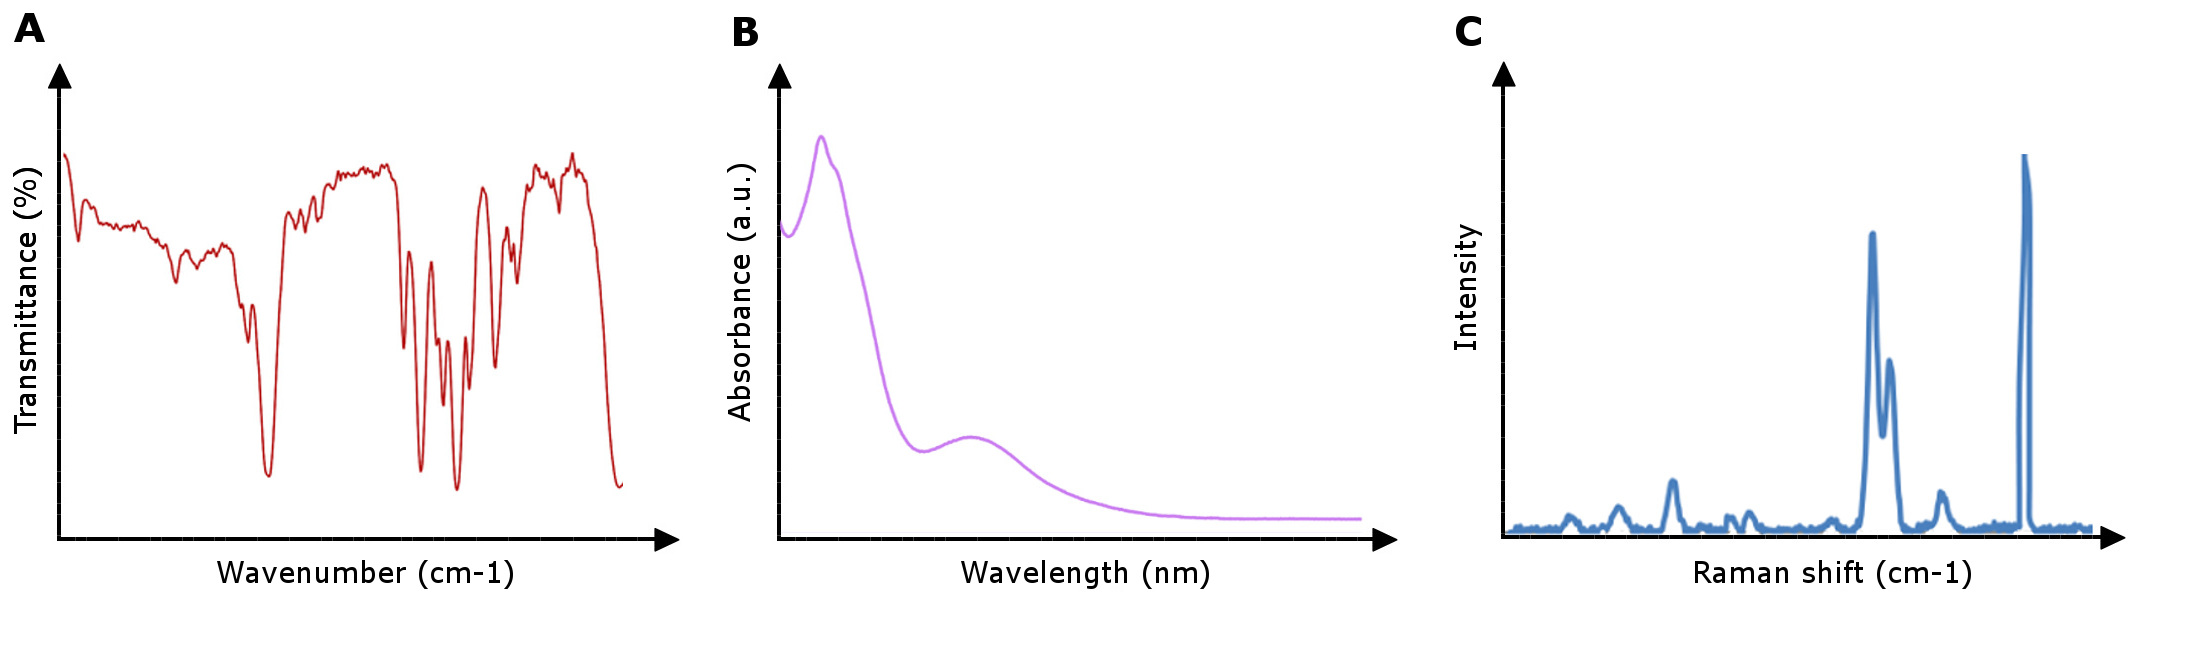
\includegraphics[width=1.1\linewidth]{Imagens/spectroscopies}
	\caption{Example of \acrshort{ir} (\textbf{A}), \acrshort{uv} (\textbf{B}) and Raman (\textbf{C}) spectra with commonly used units represented in the axis.}
	\label{spectra}
\end{figure}

\subsection{Raman Spectroscopy}

Spectroscopies such as Raman are employed to detect vibrational, rotational, and other low-frequency modes in a system. It is widely used to provide information on chemical structures and physical forms, in fingerprinting experiments and even to determine quantitatively or semi-quantitatively a compound in a sample. When light interacts with matter, the photons which make up the light can either be transmitted, reflected, absorbed or scattered, and it is this last tiny portion of light that Raman spectroscopy utilizes.

This technique uses a single frequency of radiation to irradiate the sample, and it is the radiation scattered from the molecule, one vibrational unit of energy different from the incident beam, which is detected. Most of the scattered light does not change its wavelength in the process (Rayleigh scattering) but part of it does, and such scattering is known as Raman scattering. The theory is that Raman scattering of monochromatic light (usually from a laser in the \gls{nir} or \gls{uv} range) is caused by excitations in the system, which result in the energy of the laser photons being shifted up or down. The intensity of the scattered light is plotted against its frequency ($ cm^{-1} $) and the result is a Raman spectrum of the sample (\textbf{\autoref{spectra}C}).

Compared to \gls{ir} spectroscopy, this technique is less widely used, largely due to problems with sample degradation and fluorescence. However, recent advances in instrument technology have simplified the equipment and reduced the problems substantially. These advances, together with the ability of Raman spectroscopy to examine samples in a wide range of states and minimal spectrum manipulation need, have led to a rapid growth in the application of the technique (\textbf{\autoref{spectroscopies}}) \citep{smith2005modern}.

Raman spectroscopy has been widely applied in the forensics area, having proven to be a powerful tool in the identification of body fluids \citep{virkler2010raman, sikirzhytski2010discriminant, sikirzhytski2012advanced}. The pharmaceutical industry also makes use of this technique, addressing problems such as the detection of counterfeit products \citep{roggo2010identification, sacre2011detection} and qualitative and quantitative detection of a mycotoxin in ground maize samples \citep{lee2013application}.




\setcounter{table}{0} %começava em 2 
\newcommand{\htab}[1]{\textbf{{\footnotesize \textcolor{white}{#1}}}}
\definecolor{airforceblue}{rgb}{0.36, 0.54, 0.66}

\begin{scriptsize}
	\begin{longtable}{|m{1.5cm}|m{3cm}|m{1.5cm}|m{4cm}|m{4cm}|}
		%FIRST HEADER------
		\caption{Applications of \acrshort{ir}, \acrshort{uv} and Raman spectroscopies.} 
		\label{spectroscopies} \\
		\rowcolor{airforceblue}
		\htab{Reference} & \htab{Description} & \htab{Techniques} & \htab{Preprocessing} & \htab{Analysis} \\
		\hline
		\endfirsthead
		
		%SECOND HEADER------
		\caption[]{Applications of \gls{ir}, \gls{uv} and Raman spectroscopies. (Continued)} \\
		\rowcolor{airforceblue}
		\htab{Reference} & \htab{Description} & \htab{Techniques} & \htab{Preprocessing} & \htab{Analysis} \\
		\hline
		\endhead
		
		%TABLE--------------
		
		\cite{polshin2011beer} & Prediction of important beer quality parameters & \gls{ftir} & \gls{msc}, Baseline correction, \gls{snv}, 1st
		and 2nd Savitzky-Golay derivatives, Mean centering & \gls{pca}, \gls{plsr} \\ 
		
		\hline 
		\cite{lin2005rapid} & Discrimination of \textit{Alicyclobacillus} strains in apple juice & \gls{ftir} & Spectra smoothing, 2nd derivative, Normalization & \gls{pca}, \gls{simca} \\ 
		
		\hline 
		\cite{norazian2012hybrid} & Classification of honey according to the adulteration level & \gls{ftir} & Baseline correction, Normalization, Peak correction, Outlier removal  & \gls{pca}, \gls{lda},  \\ 
		
		\hline 
		\cite{santos2013rapid} & Detection and quantification of milk adulteration & \gls{mir} & Normalization, 2nd derivative (Savitzky-Golay), Mean centering & \gls{simca}, \gls{plsr} \\ 
		
		\hline 
		\cite{cozzolino2006combining} & Differentiation of different \textit{Saccharomyces cerevisiae} strains & \gls{nir} & Autoscaling, Centering, 2nd derivative & \gls{pca}, \gls{lda} \\ 
		
		\hline 
		\cite{khairudin2014direct} & Discrimination of \textit{Polygonum minus} populations & \gls{ftir} & Pareto scaling & \gls{pca}, \gls{plsda} \\ 
		
		\hline 
		\cite{uarrota2014metabolomics} & Identification of changes and discrimination of cassava samples undergoing \gls{ppd} & \gls{ftir} & Normalization, Baseline correction & \gls{pca}, \gls{plsda}, Hierarchical clustering, \gls{svm}, One-way \gls{anova} \\ 
		
		\hline 
		\cite{preisner2007fourier} & Discrimination between different types of the \textit{Enterococcus faecium} bacterial strain & \gls{ftir} & 1st
		and 2nd Savitzky-Golay derivatives, \gls{msc}, \gls{snv}, Mean centering, Outlier removal & \gls{dipls}, \gls{plca} \\ 
		
		\hline 
		\cite{de2011barcoding} & Identification of fly species in the genus \textit{Neodexiopsis Malloch} & \gls{nir} & Savitzky-Golay derivative and smoothing & \gls{pca}, \gls{pls} \\ 
		
		\hline 
		\cite{kumar2013discrimination} & Discrimination of tea varieties & \gls{nir}, \newline \gls{uv} & Normalization & \gls{pca}, K-means clustering, \gls{pnn}, \gls{ann} \\ 
		
		\hline 
		\cite{souto2010uv} & Classification of coffee extracts according to type and conservation state & \gls{uv} & None & \gls{pca}, \gls{simca}, \gls{spalda} \\ 
						
		\hline 
		\cite{pereira2011madeira} & Prediction of wine aging & \gls{uv} & Mean centering, Smoothing, 1st and 2nd derivatives, \gls{snv}, \gls{osc} & \gls{plsr} \\ 
		
		\hline 
		\cite{urbano2006ultraviolet} & Differentiation and classification of wines & \gls{uv} & 1st derivative & \gls{pca}, \gls{simca} \\ 
		
		\hline 
		\cite{barbosa2007uv} &  Discrimination between classes of tequila & \gls{uv} & 1st derivative, Centering & \gls{pca}, \gls{plsda} \\ 
		
		\hline 
		\cite{thanasoulias2003multivariate} & Forensic discrimination of blue ball-point pen inks & \gls{uv} & Normalization & K-means cluster analysis, \gls{pca}, \gls{da} \\ 
		
		\hline 
		\cite{thanasoulias2002application} & Forensic soil discrimination & \gls{uv} & Normalization & K-means cluster analysis, \gls{pca}, \gls{da} \\ 
		
		\hline 
		\cite{virkler2010raman} & Forensic body fluid identification (blood) & \gls{nir}, \newline Raman & Normalization & \gls{sfa}, \gls{pca}, \gls{als} \\ 
		
		\hline 
		\cite{sikirzhytski2010discriminant} & Forensic identification of blood, semen and saliva stains & Raman & None & \gls{da}, \gls{simca}, \gls{lda}, \gls{plsda} \\ 
		
		\hline 
		\cite{sikirzhytski2012advanced} & Identification of body fluid traces (semen and blood) & \gls{nir}, \newline Raman & Cosmic ray interference removal, Normalization, Baseline correction & \gls{pca}, \gls{sfa}, \gls{svm} \\ 
		
		\hline 
		\cite{roggo2010identification} & Identification of pharmaceutical tablets & Raman & Cosmic ray interference removal, \gls{snv} normalization, Scaling, Mean centering, Savitzky-Golay 1st derivative & \gls{svm} \\ 
		
		\hline 
		\cite{sacre2011detection} & Detection of counterfeit Viagra{\textregistered} & Raman & Normalization & \gls{pca}, \gls{simca}, \gls{knn}, \gls{lda} \\ 
		
		\hline 
		\cite{lee2013application} & Qualitative and quantitative detection of a mycotoxin in ground maize samples & Raman & Background correction, Baseline correction, Normalization, Savitizky-Golay smoothing, Peak deconvolution & \gls{knn}, \gls{lda}, \gls{plsda}, \gls{mlr}, \gls{plsr}, Cluster analysis \\ 
		
		\hline 
		
	
	\end{longtable}
\end{scriptsize}






			

	% CHAPTER - State of the Art (workflow) ---------------------
	
	
\section{Workflow Of A Metabolomics Experiment}

Regarding metabolomics, there are four conceptual approaches: target analysis, metabolite profiling,  metabolomics, and metabolic fingerprinting \citep{roessner2009metabolomics}. The general workflow of the various metabolomics approaches is shown in \autoref{workflow}. Target analysis includes the determination and quantification of a small set of known metabolites, also called targets, making use of one particular analytical technique that shows the best performance for the compounds of interest. It has been applied for many years, including, for instance, in the analysis of head and neck cancer cells \citep{hu2015targeted}.

Metabolite profiling is different than the previous approach in the sense that it aims at the analysis of a larger set of compounds. Regarding their chemical structure, these compounds are both identified and unknown and their quantification either quantitative or semi-quantitative (an absolute quantification is not required). This approach is widely applied and has been used for instance in the identification of kidney cancer using urine's metabolic signatures \citep{kind2007comprehensive}.

The metabolomics approach employs complementary analytical methodologies, including \gls{lcms}, \gls{gcms} and/or \gls{nmr} techniques, to determine and quantify as many metabolites as possible. Similarly to the previous approach, the compounds can be either identified or unknown. It is widely used, having been applied in the determination of natural stress influence on the metabolic status of sea snail \citep{rosenblum2005characterizing}.

Lastly, in a metabolic fingerprinting approach, a metabolic "signature" or mass profile of the sample of interest is generated and then compared in a large sample population to screen for differences between the samples, it is most typically used for sample classification based on its spectrum. If the metabolites to analyze are either external and/or secreted by the cells then it is called footprinting approach. If signals that can significantly discriminate between samples are detected, then the metabolites can be identified and the biological relevance of that compound elucidated, saving valuable analysis time. It is commonly used in forensics, among other fields, having been applied for instance in the discrimination of blue ball-point pen inks \citep{thanasoulias2003multivariate}. This approach will be emphasized throughout this dissertation.

The main steps in a metabolic fingerprinting experiment are: sample preparation, data acquisition, pre-processing, data analysis and data interpretation. Upon sample preparation and data acquisition the data is then preprocessed to allow an improved analysis, where the objective is to extract useful knowledge from the data. The pre-processing and analysis steps will be the main focus throughout this dissertation.

\begin{figure}[!ht]
	\centering
	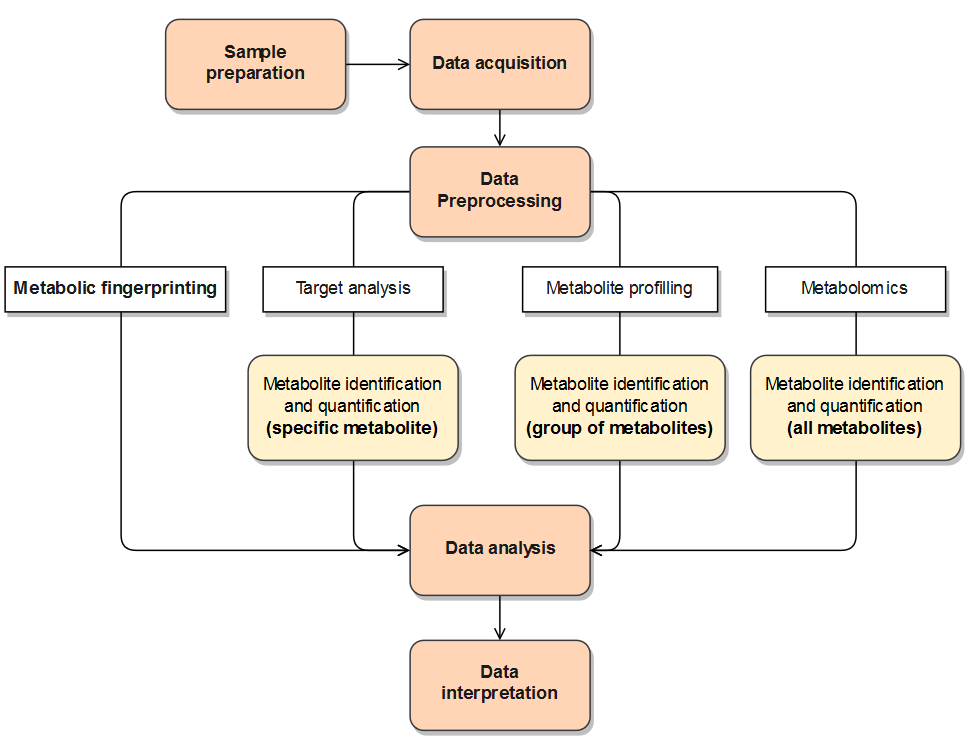
\includegraphics[width=0.9\linewidth]{Imagens/workflow}
	\caption{General workflow of the various metabolomics approaches.}
	\label{workflow}
\end{figure}


\subsection{Preprocessing}

The pre-processing step covers all editing of the data up to the point of starting the analysis. This is a crucial step in any metabolomics experiment, making samples analyzable and comparable. In a metabolic fingerprinting approach, the most commonly used pre-processing methods include missing values and outlier removal, normalization or scaling, derivative calculation, mean centering and some peak spectra processing. The order in which the pre-processing steps are applied to the data is not always obvious, being sometimes governed more by practical considerations than optimal statistical analysis. The methods discussed in this section are the ones most commonly used regarding \gls{ir}, \gls{uv} and Raman spectroscopies, the techniques focused on this dissertation.

When handling missing values, there are two main approaches: their removal or replacement. In the first approach, the value can be removed by either removing the feature or the sample containing it. In the latter, the value can be replaced using various methods, including its replacement by the row or column mean, or even using more sophisticated methods (e.g. nearest neighbors, linear approximation). Frequently, there are values within the dataset that are distant from all other observations, thus considered outliers. These are typically excluded from the dataset, as they could interfere in the subsequent analysis results.

Peak spectra pre-processing aims to perform corrections over the spectra. It includes for instance baseline and background correction and smoothing methods, among others. Baseline correction method is used to correct unwanted linear or non-linear additions to the spectra. These additions are often associated with equipment used when measuring samples (e.g. non-linearities in detectors) or, for instance, by the interference of a complex matrix. Depending on the situation, this method might be essential, considering most statistical analysis techniques cannot distinguish between baselines and signal. 

Background correction, as the name suggests, is applied to remove the background in the spectra. This background can be caused by various factors, including absorption associated with the sample holder and/or solvent used. 

The smoothing methods are used to filter spectra noise, and might be specially helpful when signal-to-noise ratio is high or the subsequent analysis methods are very sensitive to noise. It helps in both visual interpretation and robustness of the analysis, but it is important to balance noise reduction and peak retention, specially in the small peaks \citep{liland2011multivariate}. The Savitzky-Golay filter is one of the most popular smoothing methods. This method fits successive sub-sets of adjacent data points with a low-degree polynomial by the method of linear least squares, using a process known as convolution \citep{savitzky1964smoothing}.

Other commonly used peak spectra pre-processing methods include peak alignment and binning. In its simplest form, peak alignment consists in dividing the spectra in a number of local windows, where peaks are shifted to match across spectra. Since everything is done locally, peak alignment is a fast method, however, it may lead to misalignment when peaks fall into the wrong local window or are split into two windows. When continuous spectra are recorded producing tens or hundreds of thousands of measurements per spectrum, the binning method can be helpful. In this method, the spectrum is divided into a desired number of bins and all measurements inside each bin summed, forming new spectra with fewer variables. The simplest reason for binning is that the number of variables can be too high for handling of the problem in ordinary computer memory. There are, however, a few dangers regarding the bad placing of the bins, by removing information or producing false information \citep{liland2011multivariate}.

In many analytical methods, the variables measured for a given sample are subject to overall scaling or gain effects. Standardization methods attempt to correct for these kinds of effects by identifying some aspect of each sample which should be essentially constant between samples, giving all them an equal impact on the model. In the \acrfull{snv} method, a weighted normalization is performed (not all points contribute to the normalization equally). Therefore, the values are subtracted of their mean and then the result is divided by the standard deviation. Spectra treated in this manner have always zero mean value and a variance equal to one and are thus independent of original absorbance values. 

The \acrfull{msc} method is a relatively simple processing step that attempts to account for additive and/or multiplicative effects in spectral data. It does so by estimating light scattering or change in path length for each sample relatively to that of an ideal sample. Another method consists in centering the data, by calculating the average spectrum of the dataset and subtracting that average from each spectrum. In this method, the values are changed, but not the scale.

Derivative spectroscopy uses first or higher derivatives of absorbance with respect to wavelength for qualitative analysis and for quantification. Generally speaking, by differentiation of a zero order spectrum and obtaining consecutive derivative spectra the separation of overlapping peaks is achieved, increasing selectivity without separation of the analytes. First and second-order derivatives are the ones most commonly calculated. A graphical representation of first and second order derivatives calculation is shown in \autoref{derivatives}. The first-order derivative consists in the rate of change of absorbance with respect to wavelength, while the second-order derivative has a very characteristic feature consisting in a negative band with minimum at the same wavelength as the maximum on the original spectrum. This method can be useful because spectra that are very similar in absorbance mode may reveal significant differences in the derivative mode. Another advantage resides in the fact that because the first derivative of a constant absorbance offset is zero, calculating the first derivative spectra always eliminates baseline shifts \citep{kus1996derivative}.

\begin{figure}[!htb]
	\centering
	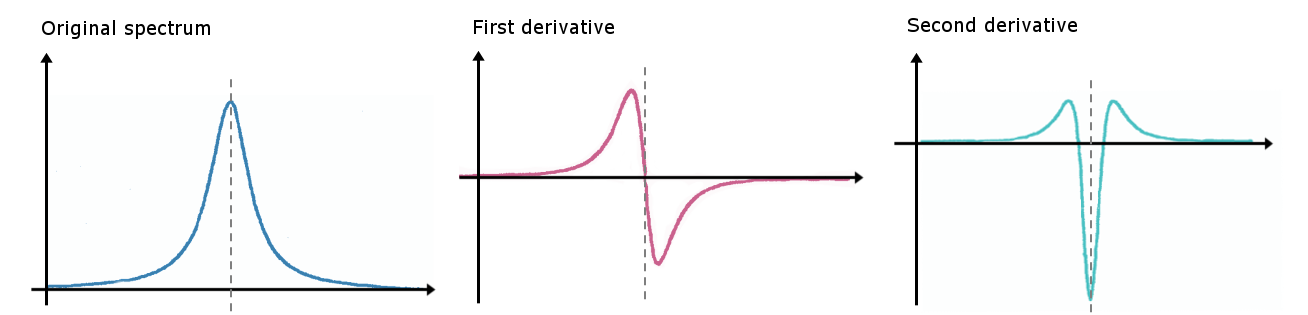
\includegraphics[width=1\linewidth]{Imagens/derivatives}
	\caption{Graphical representation of first and second order derivatives calculation.}
	\label{derivatives}
\end{figure}


The pre-processing methods applied can vary greatly between datasets and type of spectroscopy used. \textbf{\autoref{spectroscopies}} summarizes the various pre-processing methods used in several experiments from the literature (in the fourth column). In \gls{ir} spectroscopy, peak spectra processing methods are often applied, including smoothing and baseline correction. Normalization and scaling methods, including mean centering and \gls{snv} are also often used, as well as first and second-order derivatives calculation. Unlike \gls{ir} spectroscopy, in \gls{uv} experiments less pre-processing methods are applied, being normalization and first derivative calculation the most commonly applied methods. In Raman spectroscopy, the pre-processing methods usually applied are similar to those applied in \gls{ir} spectroscopy.






	
\subsection{Univariate data analysis} \label{univariate}

After the pre-processing step, the data is finally ready to be analyzed. This dataset is usually under the form of a matrix, with either a compound list or a peak list and their values for different samples. The main types of data analysis are: univariate analysis, unsupervised multivariate techniques and supervised multivariate techniques (machine learning).

Univariate analysis investigates each variable separately or relates a single independent variable $ x $ to a single dependent variable $ y $. However, the data obtained from experiments regarding compounds, reactions and/or samples are multivariate in nature, which means a good characterization often requires using many variables simultaneously. Multivariate data analysis considers many variables together and thereby often gains a new and higher quality in data evaluation. The differences between supervised and unsupervised methods relies in the fact that the first ones do not need any metadata (e.g. information about natural groups within the data), while the latter requires samples to be divided into at least two classes (or groups) to allow the methods to conduct a learning (or training) process \citep{varmuza2009introduction}.

This section will cover univariate analysis techniques, whereas unsupervised multivariate techniques and supervised multivariate techniques will be explored with further detail in \autoref{unsupervised} and \autoref{supervised}. 

Among the most popular univariate analysis techniques used in metabolic fingerprinting approaches are the t-tests, \acrfull{anova} and fold change analysis. Non-parametric tests often used include the Kruskal-Wallis, Kolmogorov-Smirnov and Wilcoxon signed-rank tests. Regression analysis is also often employed. 

A t-test is a statistical hypothesis test in which the test statistic follows a Student's t distribution under the null hypothesis. It allows for data comparison, by determining if two sets of data are significantly different from each other. This test is most commonly used to test whether the mean of a population can have a specified value, to test if the means of two populations can be equal (two-sample test), to test whether the slope of a regression line differs significantly from 0, among other uses.

The \gls{anova} is a collection of statistical models used to assess the relative size of variance among group means compared to the average variance within groups. For a comparison of more than two group means, the one-way \gls{anova} is the appropriate method instead of the t-test. It is similar to multiple two-sample t-tests, but since it is less conservative (results in a smaller number of type I errors) it is suited to a wide range of practical problems. The two-way \gls{anova} is an extension of the one-way \gls{anova} and it examines the influence of two different categorical independent variables on one continuous dependent variable. Besides assessing the main effect of each variable, it also assesses if there is any interaction between them.

The degree of how relatively greater the difference is between group means compared to within group variance is known to follow the F distribution. Therefore, the \gls{anova}  makes use of the F-test to test the statistical significance by comparing the F statistic, which compares the variance between groups with the variance within groups. If any significant difference is detected by the F-test, the specific pair of group means that show differences and the pairs that do not can be examined using a post-hoc test. One such test for this task is the Tukey's \gls{hsd} test \citep{kim2014analysis}.

When conducting multiple comparisons, as is the case of a metabolic fingerprinting experiment, the \gls{fdr} is one way of conceptualizing the rate of type I errors (false positives) in null hypothesis testing. This method provides a less stringent control of Type I errors when compared to familywise error rate controlling procedures (e.g. Bonferroni correction).

The \gls{fc} is calculated by getting the ratio between the mean value of the selected variable in one group in comparison to the same value in another group, thus measuring how much a variable mean changes within two groups. It is an interesting measure in the sense that it allows for group discrimination according to the selected feature, given that the \gls{fc} value is significant enough (usually \gls{fc} $ \textgreater $ 2).

Many statistical tests rely heavily on distributional assumptions, such as normality. However, when these assumptions are not satisfied, commonly used statistical tests often perform poorly, resulting in a greater chance of committing an error. Non-parametric tests are designed to have desirable statistical properties when few assumptions can be made about the underlying distribution of the data. In other words, when the data are obtained from a non-normal distribution or one containing outliers, a non-parametric test is often a more powerful statistical tool than it's parametric equivalent.

The Kruskal–Wallis H-test for one-way \gls{anova} by Ranks is often viewed as the nonparametric equivalent of the parametric one-way \gls{anova}. As a nonparametric test, it uses ranked data, and is particularly employed when: the data are ordinal and do not meet the precision of interval data; there are serious concerns about extreme deviation from normal distribution; and there is considerable difference in the number of subjects for each comparative group. This test is frequently used for when it is necessary to determine if three or more independent samples originate from the same population. A significant Kruskal-Wallis test indicates that at least one sample stochastically dominates one other sample. The test does not identify, however, where this stochastic dominance occurs or for how many pairs of groups stochastic dominance obtains.

Kolmogorov-Smirnov Two-Sample test is another nonparametric test often used to determine if two independent samples are taken from either the same population or from two populations that have the same distribution pattern. It is sensitive to distribution differences, either in central tendency or dispersion differences, being more useful when these differences are due more to the latter case. The Kolmogorov-Smirnov test uses ordinal data and is especially useful with small samples, such as when there are fewer than 40 subjects in each of the two samples.

The Wilcoxon Signed-Rank test is a nonparametric hypothesis test often viewed as being similar to Student's t-test for matched pairs, but it is used for ordinal data or data that seriously violate any semblance of normal distribution. This method is employed when comparing two related samples (matched samples) or repeated measurements on a single sample to assess whether their population mean ranks differ (i.e. it is a paired difference test), focusing on both the magnitude and direction of the differences for matched pairs \citep{macfarland2016introduction}.

Perhaps the most widely used statistical technique is Regression analysis. Linear regression analysis allows the investigation and modeling of the relationship between a scalar dependent variable $ y $ and one or more independent variables (regressors) denoted $ x $, assuming a linear relationship between them. This relationship is estimated through a mathematical equation (i.e. a linear model) which, in its most general form looks like:

\begin{equation}
	\centering
	\label{regression}
		y_{i} = \beta_{0} + \beta_{1}x_{i1} + ... + \beta_{p}x_{ip} + \varepsilon_{i},	\hspace{15mm}	i = 1,...,n
\end{equation}
 
where $ y_{i} $ represents the dependent variable, $ x_{i1} - x_{ip} $ the independent variables, $ \beta $ is a $ p $-dimensional parameter vector and its elements called regression coefficients and, lastly, $ \varepsilon_{i} $ represents the error term. In almost all applications of regression, the regression equation is only an approximation to the true functional relationship between the variables of interest and are valid only over the region of the regressor variables contained in the observed data.

The case when there is only one independent variable is called simple linear regression, whereas for more than one independent variable the process is called multiple linear regression. The regression coefficients are often estimated using the least squares method, which attempts to minimize the sum of the squares of the errors made in the results of every single equation \citep{darlington2016regression}.






	
\subsection{Unsupervised methods} \label{unsupervised}

Among the most commonly used unsupervised methods there are \acrfull{pca} and clustering methods such as \acrfull{hca} and the k-means method.

The \gls{pca} is a statistical procedure whose principal aim is to reduce data dimension, by converting a set of observations of possibly correlated variables into a set of values of linearly uncorrelated variables (principal components). It aims to explain as much data variability as possible with as few principal components as possible. In general, principal components can be computed up to the total number of variables. It can be seen as a method to compute a new coordinate system formed by the latent variables, which is orthogonal, and where only the most informative dimensions are used. Latent variables from PCA optimally represent the distances between the objects in the high-dimensional variable space.

The results of a \gls{pca} analysis include the scores of the supplied data on the principal components (i.e. the transformed variable values that corresponds to a particular data point), the matrix of variable loadings, corresponding to the weights of each original variable on the new coordinates and the standard deviations (or variance) explained by each of the principal components (or cumulative). In this method, it is generally recommended to use mean-centered data, and because it is also sensitive with respect to outliers, robust \gls{pca} can be used \citep{varmuza2009introduction}.

Cluster analysis tries to identify concentrated groups (clusters) of objects, without prior information about any group membership and/or number of clusters. In other words, cluster analysis tries to find groups containing similar objects, and usually one cannot expect a unique solution for cluster analysis. There are two main types of clustering methods, namely hierarchical and non-hierarchical clustering.

In the \acrfull{hca}, objects and partitions are arranged in a hierarchy and represented in a tree-like dendrogram, being a complementary, nonlinear, and widely used method for cluster analysis (\autoref{clustering}). Strategies for \gls{hca} generally fall into two types: agglomerative and divisive clustering. 

\begin{figure}
	\centering
	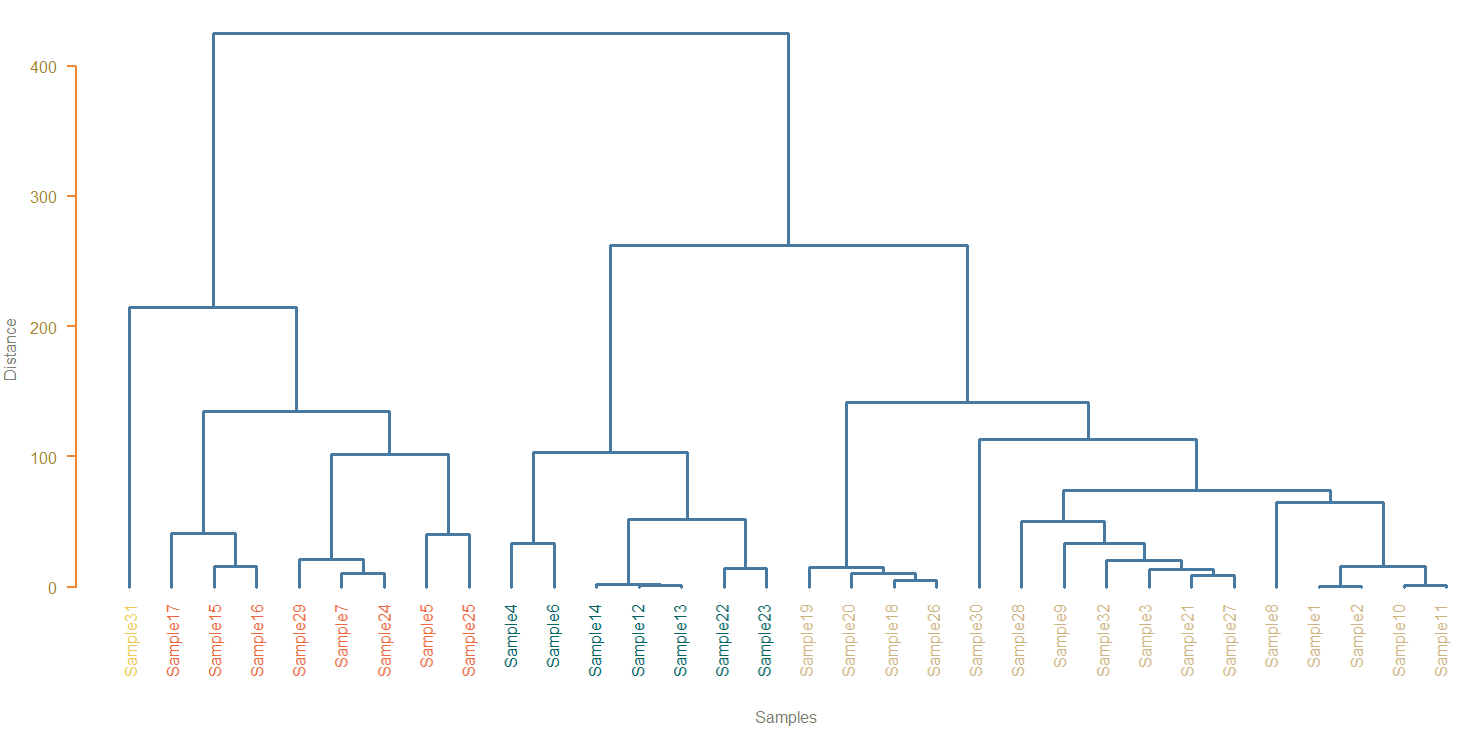
\includegraphics[width=1\linewidth]{Imagens/clustering}
	\caption{Example of a dendrogram resulting from a cluster analysis performed over 32 samples. The distance between samples is represented in the $ y $ axis, whereas sample names are represented in the $ x $ axis.}
	\label{clustering}
\end{figure}


In the first approach, each of the $ n $ objects forms a separate cluster, resulting in $ n $ clusters in the first level. In the next level the two closest clusters are merged, and so on, until finally all objects are in one single cluster. The divisive method groups all $ n $ objects in one single cluster, in the first level of the hierarchy. In the next level, this cluster is split into two smaller clusters, and so on, until finally each object forms a separate cluster. Usually one cannot expect a unique solution for cluster analysis. The result greatly depends on the used distance measure (e.g. Euclidean or Manhattan distances), the cluster algorithm (e.g. Nearest Neighbor or complete linkage), and the chosen parameters \citep{varmuza2009introduction}.

Unlike \gls{hca}, non-hierarchical clustering methods aim to partition a dataset into a pre-defined number of clusters, organizing data objects into a set of typically non overlapping flat groups, by typically using iterative algorithms that optimize a chosen criterion. One of the most used non-hierarchical clustering formulations is the k-means clustering. An algorithm for this approach starts from a set of initial random clusters, then proceeding to take each point belonging  to a  given data set and associate it to the nearest center, minimizing the distance of the observation to the cluster mean. This last step is repeated until no improvement in the objective function can be made. This algorithm (named Lloyd algorithm) is usually fast, however, given that it is an heuristic algorithm, there is no guarantee that it will converge to the global optimum, and the result may depend on the initial set of clusters.





	
\subsection{Supervised methods: machine learning} \label{supervised}

Machine learning techniques are often used when performing a metabolic fingerprinting experiment. It focuses on the construction of algorithms that can learn from and make predictions on data, through building a model from sample inputs. In order to build a predictive model, a set of training data must be provided, and the learner algorithm must have the ability to generalize from its experience, by performing accurate predictions on new, unseen examples. 

In machine learning, tabular data is the most common way of representing the data. It consists in a data table with rows representing the different samples, or X, and a single or multi-column property, or y, that is known for each example (\autoref{tabular_data}). The properties are usually the interesting facts of the examples. When properties are of continuous nature it is called a regression approach, whereas if they are of discrete nature it is called a classification approach \citep{varmuza2009introduction}. The general workflow of a machine learning approach is represented in \autoref{ml_workflow}.

\begin{figure}[!htb]
	\centering
	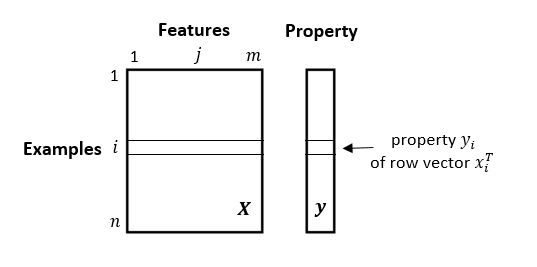
\includegraphics[width=0.6\linewidth]{Imagens/tabular_data}
	\caption{Graphical representation of tabular data used in a machine learning approach, including feature matrix X and a property vector y.}
	\label{tabular_data}
\end{figure}



Among the most popular supervised methods for classification are: \acrfull{plsda}, \acrfull{lda}, \acrfull{simca} and Decision trees. Methods for regression tasks include \acrfull{plsr} and Regression trees. Methods such as \acrfull{knn}, \acrfull{svm}, \acrfull{ann} and Random Forests can be used for both classification and regression tasks.

\acrfull{pls} is a method to relate a matrix X of independent variables to a vector y or to a matrix Y of dependent variables. In the model structure of \gls{plsr}, the X-data is first transformed into a set of intermediate linear latent variables (components). Since it is a linear method, the final latent variable that predicts the modeled property, y, is a linear combination of the original variables. During model development, a relatively small number of \gls{pls} components are calculated, and it is the number of such components that determines the complexity of the model, which can be optimized for high prediction performance. \gls{plsda} is a variant used when the Y is categorical \citep{varmuza2009introduction}.

\begin{figure}
	\centering
	\includegraphics[width=0.85\linewidth]{Imagens/ml_workflow}
	\caption{General workflow of a machine learning approach.}
	\label{ml_workflow}
\end{figure}

\gls{lda} attempts to find a linear combination of features (latent variable) that characterizes or separates two or more classes of objects or events. The resulting combination is commonly used as a linear classifier. The representation of a \gls{lda} model consists of statistical properties of the data, which are calculated for each class and then used to make predictions. For a single input variable, $ x $, these properties are the mean and the variance of the variable for each class, whereas for multiple variables the properties consist in the means and covariance matrix. This method assumes a Gaussian distribution of the data and that each attribute has the same variance. It is closely related to \gls{pca}, although \gls{pca} does not take into consideration the underlying class structure, being sometimes used for data dimensionality reduction \citep{martinez2001pca}.

The \gls{simca} method is based on disjoint principal component models. The idea is to describe the multivariate data structure of each group separately in a reduced space using \gls{pca}. The special feature of this method, is that \gls{pca} is applied to each group separately and also the number of principal components is selected individually and not jointly for all groups.  Due to the use of \gls{pca}, this approach works even for high-dimensional data with rather a small number of samples, whereas methods like \gls{lda} can become unstable under such conditions. In addition to the group assignment for new objects, \gls{simca} also provides information about the relevance of different variables to the classification, or measures of separation \citep{varmuza2009introduction}.

Decision trees consist in a flowchart-like structure in which internal nodes represent the test on an attribute, the branches represent the outcome of the test and the leaves represent a class label. The learning phase is done by splitting the source set into subsets based on an attribute value test, repeating this process in a recursive manner until the subset at a node has the same value of the target variable, or when splitting no longer adds value to the predictions. When the target variable is of discrete nature it is called a classification tree, whereas when the target variable is of continuous nature it is called a regression tree. A Random Forest classifier builds a large collection of uncorrelated trees, and then averages them to improve the classification rate. It uses the bagging method which helps to reduce variance and corrects the decision's tree habit of overfitting to their training set \citep{friedman2009elements}.

In contrast to the already mentioned machine learning methods, the \gls{knn} method does not require a model to be fit. It is a type of lazy learning method, where the function is only approximated locally and all computation is deferred until classification. For \gls{knn} classification, the task is to predict the class membership of a new object $ x $. Using, for instance, the Euclidean distance measure, the k-nearest neighbors (of the training data) to $ x $ are determined. The neighbors are found by calculating the distances between the new object and all objects in the training set. This method has the advantage of neither requiring linearly separable groups nor compact clusters for the groups, being easily applied to multi-class problems \citep{varmuza2009introduction}.

Given a set of training examples and two possible categories for each example, the \gls{svm} algorithm builds a model capable of assigning examples to one of the two categories, making it a non-probabilistic binary linear classifier. It produces linear boundaries between object groups in a transformed space of the $ x $-variables, usually of much higher dimension than the original $ x $-space. These class boundaries are constructed to maximize the margin between the groups. New examples are then mapped into that same space and predicted to belong to a category based on which side of the decision boundary they fall \citep{varmuza2009introduction}.

In \gls{ann}s, the central idea is to extract linear combinations of the inputs as derived features, and then model the target as a nonlinear function of these features. An \gls{ann} is a two-stage regression or classification model, typically represented by a network diagram, where neural units are interconnected. This network usually has three layers, consisting in an input layer, an hidden layer and an output layer. The input data goes into the first layer, the hidden layer nodes do some calculations and then the output is gathered from the last layer. The links between different neural units can be enforcing or inhibitory in their effect on the activation state of connected neural units, usually through a limiting (threshold) function \citep{friedman2009elements}.

Some of these (and other) machine learning methods used in spectral data analysis studies available in the literature are listed on the fifth column of \autoref{spectroscopies}.






	
\subsection{Feature selection}

Machine learning methods have a difficulty in dealing with the large number of input features and, therefore, pre-processing of the data is essential to use these methods effectively. Feature selection is an important technique which has become indispensable in the machine learning process. It consists in   the process of detecting relevant features and removing irrelevant, redundant, or noisy data. This technique greatly speeds up machine learning algorithms, also improving predictive accuracy and comprehensibility.

There are three feature selection approaches: filters, wrappers and embedded methods. The filter approach incorporates an independent measure for evaluating features subsets without involving a learning algorithm. This method can, however, miss features that are not useful alone but can be very useful in combination with others. On the other hand, the wrapper approach uses a learning algorithm for subset evaluation. This method thus selects an optimal subset that is best suited to the learning algorithm having, therefore, a better performance when compared to the filter approach in most cases. Embedded methods have been recently proposed and try to combine the advantages of both previous methods. In this method, the learning algorithm takes advantage of its own variable selection process and performs feature selection and classification simultaneously \citep{kumar2014feature}. A graphical representation of filter, wrapper and embedded approaches is shown in \autoref{feature_selection}.


\begin{figure}[!htb]
	\centering
	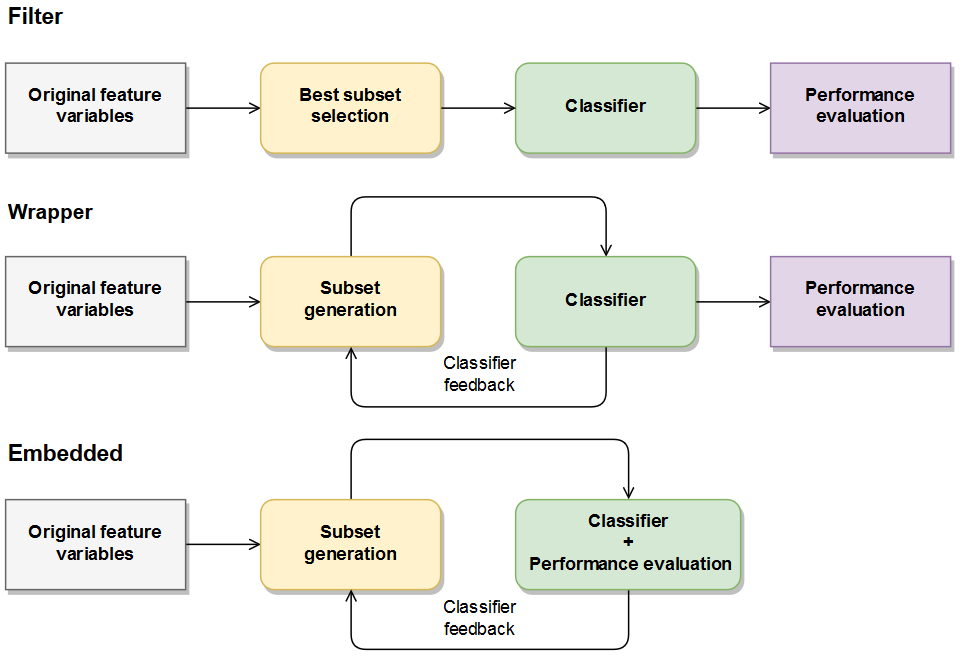
\includegraphics[width=0.85\linewidth]{Imagens/feature_Selection}
	\caption{Workflow of Filter, Wrapper and Embedded approaches in feature selection.}
	\label{feature_selection}
\end{figure}

Filter approaches are based on statistical tests (e.g. chi-squared test) measuring some intrinsic properties of the dataset (or features), including information gain, variance threshold and the correlation coefficient. The latter method was used for instance in the predictive biomarker discovery in biological samples \citep{grissa2016feature}.

Wrapper methods include \gls{rfe}, \gls{sfs} algorithms and \gls{ga}. The \gls{rfe} method uses all initial features to fit the model, ranking all features according to their contribution. In each subset, most relevant variables are retained and the model is refitted. This process continues until the subset with best performance is obtained. While the \gls{rfe} method uses the feature weight coefficients or feature importance, the \gls{sfs} method removes (or adds) features based on a user-defined classifier/regression performance metric, until a feature subset of the desired size k is reached. 

\gls{ga}s are metaheuristic optimization algorithms that use an initial population of candidate solutions (individuals), which is then evolved toward better solutions. This is done by an iterative process, where in each iteration (generation) the fitness (i.e. value of the objective function) of every individual in the population is evaluated. The fittest individuals are stochastically selected from the current population and recombined to form a new generation. The algorithm terminates when either a maximum number of generations has been produced, or a satisfactory fitness level has been reached for the population. This method was used for instance in bacteria discrimination using \gls{ftir} spectroscopy \citep{preisner2007fourier}.

Embedded methods use for instance decision trees and the \gls{lasso} regression algorithm for generalized linear models. \gls{lasso} penalizes the absolute size of the regression coefficients (i.e. forces their sum to be less than a fixed value), which forces certain coefficients to be set to zero. It is a convenient method for automatic feature selection when dealing with highly correlated predictors. This method has been applied for instance in the diagnosis of insulin resistance \citep{milburn2013application}.






	
	% CHAPTER - State of the Art (Data Integration)
	
	
\section{Data Fusion}

%http://www.slideshare.net/paveenju/2014-data-fusionpptx
%https://books.google.pt/books?id=6Im9BwAAQBAJ&pg=SA1-PA7&lpg=SA1-PA7&dq=data+fusion+identity+declaration&source=bl&ots=lyTWUcUAlk&sig=LhmwoIGX2SmVMMNR-OQ6exRIu1c&hl=pt-PT&sa=X&ved=0ahUKEwj6qpiI_4TRAhWEWhQKHQRmA-4Q6AEIKTAB#v=onepage&q&f=false 1-7

Data fusion is a process of combining data from different sources to improve the performance of prediction models. It deals with association, detection, correlation and estimation of data to achieve a better information of the system's state. In the fusion process, data is collected by $ N $ different source types (e.g. \gls{ir} and \gls{uv} data). The data can then be pre-processed to extract a feature vector that represents the observed data, and a machine learning approach, using the observed objects, may be performed. The output of this process must be partitioned into groups representing observations belonging to the same category and, finally, the fusion algorithms combine the multi-source data to obtain a result that has less uncertainty than it would if these sources were used individually. 

There are three main categories of data fusion, depending on the abstraction level the fusion of identity declarations takes place: \gls{llf}, \gls{ilf} and \gls{hlf}. A graphical representation of these approaches is shown in \autoref{data_fusion}.


\begin{figure}[!htb]
	\centering
	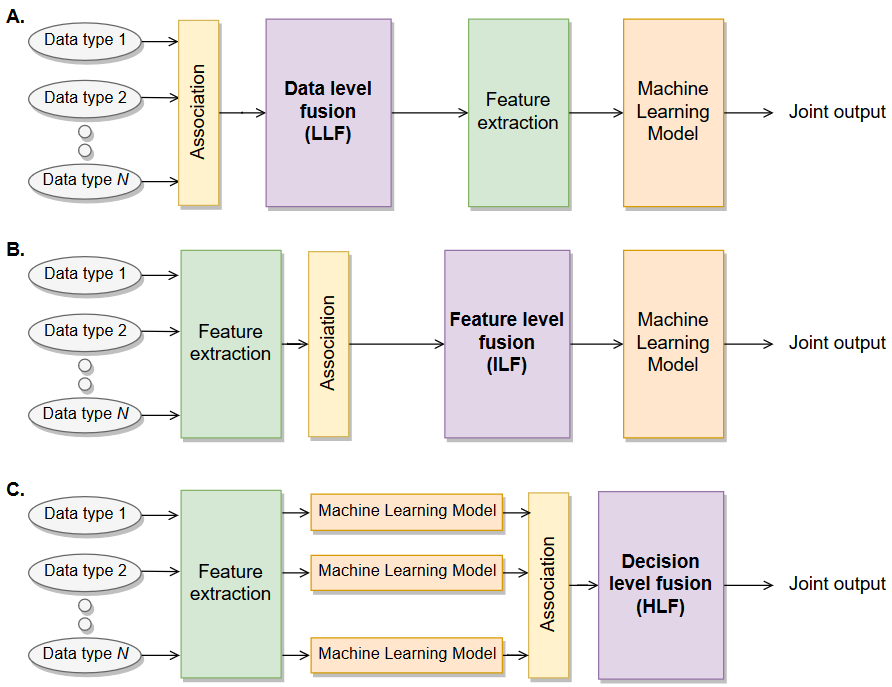
\includegraphics[width=1\linewidth]{Imagens/data_fusion}
	\caption{Graphical representation of \textbf{A.} \acrfull{llf}, \textbf{B.} \acrfull{ilf} and \textbf{C.} \acrfull{hlf}.}
	\label{data_fusion}
\end{figure}


\gls{llf} is made on a data level, by direct association and combination of raw data, representing measures of the same physical phenomena. After data combination, a feature vector is extracted and used in a machine learning process. It provides the most accurate results, assuming proper data association.

\gls{ilf} on the other hand is made on a feature level. Here, a representative features vector is extracted directly from the data. After data alignment and association, the feature vectors are concatenated into a single vector acting as an input for a machine learning process. The output is, therefore, based on the combined feature vectors from all of the data types.

Lastly, \gls{hlf} is made on a decision level. Initially, the data from each of the data types are used in a machine learning process, which can be coupled with feature extraction (e.g. using neural networks). Data association and correlation are still required to ensure that the data to be fused refer to the same physical entity. Finally, the the results from the machine learning process using each of the data types are combined using decision level fusion techniques (e.g. Bayesian inference) \citep{fourati2015multisensor}.

\gls{llf} and \gls{ilf} approaches were applied for instance in the classification of pure and adulterated honey \citep{norazian2012hybrid}. Combining e-nose and \gls{ir} data they found these two approaches achieved better results than single modality data. An \gls{hlf} approach using Bayesian inference was applied in the discrimination of white grape varieties (\gls{ftir} and \gls{uv} data), having achieved half the misclassification error when compared to the use of single modality data \citep{roussel2003fusion}.








	% CHAPTER - State of the Art (Free Software)
	
	
\section{Available Free Tools For Metabolomics and Spectral Data} \label{met_tools}

In response to the increasing growth of information output through the years, a number of computational tools for metabolomics and spectral data have become available. Among these are some interesting packages on the open-source R scientific computing platform (\href{http://www.r-project.org}{\nolinkurl{http://www.r-project.org}}), including \textit{hyperSpec} and \textit{ChemoSpec}. 

The \textit{hyperSpec} package allows convenient handling of Hyperspectral data (i.e. spectra with associated space, time or other additional information). It handles data recorded over a discretized axis, obtained from \gls{uv}, \gls{nir}, \gls{ir}, Raman and other spectroscopy techniques. It has several plot functions to display spectra, false-colour maps, calibration curves, among other purposes. Preprocessing methods include data normalization, intensity calibration, offset and baseline corrections, spectral interpolation, and many other methods. For the analysis, this package provides functions for clustering analysis, \gls{pca}, \gls{pls}, \gls{lda}, among others \citep{hyperspec}.

The \textit{ChemoSpec} package was designed with metabolomics data sets in mind, where the samples fall into groups, such as treatment and control. It consists in a collection of functions for entirely exploratory and unsupervised data analysis of spectral data, including \gls{ir}, \gls{uv} and Raman data, among other types of spectral data. It includes functions for plotting and inspecting spectra, as well as some pre-processing functions for data normalization and binning, identifying and removing problematic samples or regions of no interest, baseline correction, peak alignment, among others. Unsupervised methods such as \gls{hca}, \gls{pca} and model-based clustering are also covered in this package \citep{chemospec}.

Among web-based tools available for metabolomics and spectral data analysis the most notable and comprehensive is \textit{MetaboAnalyst}. It accepts data from either targeted profiling (concentration tables) or metabolic fingerprinting approaches (spectral bins, peak lists) produced from either \gls{nmr}, \gls{lcms} or \gls{gcms}. Preprocessing of the data is available, including normalization and scaling, data transformation, outlier removal, among other methods. The statistical analysis module offers various commonly used statistical and machine learning methods, including t-tests, \gls{anova}, \gls{pca}, \gls{plsda}, Orthogonal \gls{plsda}, and also clustering and visualization tools to create dendrograms and heatmaps as well as to classify based on random forests and \gls{svm}. \textit{MetaboAnalyst} includes modules for other types of analysis as well, including the enrichment analysis, pathway and time-series analysis modules, among others. 

\begin{table}[!ht]
	\caption{Available free tools for metabolomics and spectral data.} 
	\label{tools}
	\begin{scriptsize}
		\tabulinesep=1.2mm
		\begin{tabu}{|m{1.8cm}|m{5.2cm}|m{5cm}|m{2.4cm}|}		
			\rowcolor{airforceblue}
			\htab{Name} & \htab{URL} & \htab{Description} & \htab{Data types} \\
			\hline
			
			chemometrics & \href{https://CRAN.R-project.org/package=chemometrics}{\nolinkurl{https://CRAN.R-project.org/package=chemometrics}} & R package for multivariate statistical analysis in chemometrics & Chemical data \\ 				
			\hline 
			
			ChemoSpec & \href{https://CRAN.R-project.org/package=ChemoSpec}{\nolinkurl{https://CRAN.R-project.org/package=ChemoSpec}} & R package for exploratory analysis of spectral data & \gls{nmr}, \gls{ir} and Raman  \\ 		
			\hline 
			
			COLMAR & \href{https://spin.ccic.ohio-state.edu/index.php/colmar}{\nolinkurl{https://spin.ccic.ohio-state.edu/index.php/colmar}} & Webserver for \gls{nmr} data analysis and compound identification & \gls{nmr} \\ 
			
			\hline 
			hyperSpec & \href{https://CRAN.R-project.org/package=hyperSpec}{\nolinkurl{https://CRAN.R-project.org/package=hyperSpec}} & R package for Hyperspectral data analysis & \gls{uv}, \gls{ir}, \gls{nmr}, \gls{ms}, Raman, ... \\ 
			
			\hline 
			MeltDB & \href{https://meltdb.cebitec.uni-bielefeld.de/cgi-bin/login.cgi}{\nolinkurl{https://meltdb.cebitec.uni-bielefeld.de/cgi-bin/login.cgi}} & Web-based system for metabolomics data analysis and dataset annotation & \gls{gcms} and \gls{lcms} \\ 
			
			\hline 
			MetaboAnalyst & \href{http://www.metaboanalyst.ca}{\nolinkurl{http://www.metaboanalyst.ca}} & Web-based system for metabolomics and spectral data analysis & \gls{nmr}, \gls{lcms} and \gls{gcms} \\ 
			
			\hline
			metabolomics & \href{https://CRAN.R-project.org/package=metabolomics}{\nolinkurl{https://CRAN.R-project.org/package=metabolomics}} & R package for metabolomics data analysis & \gls{nmr}, \gls{gcms}, \gls{lcms} and \gls{ms} \\
			
			\hline 
			MetaboMiner & \href{https://wishart.biology.ualberta.ca/metabominer/}{\nolinkurl{https://wishart.biology.ualberta.ca/metabominer/}} & Java based software for \gls{nmr} data analysis and compound identification & \gls{nmr} \\ 
			
			\hline 
			metaP-Server & \href{http://metap.helmholtz-muenchen.de/metap2/}{\nolinkurl{http://metap.helmholtz-muenchen.de/metap2/}} & Web-based system for metabolomics data analysis & \gls{nmr}, \gls{gcms}, \gls{lcms} and \gls{ms} \\ 
			
			\hline 
			muma & \href{https://CRAN.R-project.org/package=muma}{\nolinkurl{https://CRAN.R-project.org/package=muma}} & R package for metabolomics univariate and multivariate analysis & \gls{nmr}, \gls{gcms}, \gls{lcms} and \gls{ms} \\ 
			
			\hline 
			MVAPACK & \href{https://bionmr.unl.edu/mvapack.php}{\nolinkurl{https://bionmr.unl.edu/mvapack.php}} & Toolkit for \gls{nmr} and \gls{ms} data handling & \gls{nmr} and \gls{ms} \\ 
			
			\hline 
			OpenMS & \href{https://www.openms.de/}{\nolinkurl{https://www.openms.de/}} & C++ library for \gls{lcms} data handling and analysis & \gls{lcms} \\ 
			
			\hline 
			specmine & \href{https://CRAN.R-project.org/package=specmine}{\nolinkurl{https://CRAN.R-project.org/package=specmine}} & R package for the integrated analysis of metabolomics and spectral data & \gls{nmr}, \gls{gcms}, \gls{lcms}, \gls{uv}, \gls{ir}, Raman, ... \\ 
			
			\hline 		
		\end{tabu}
	\end{scriptsize}
\end{table}

These and other freely available tools are listed in \autoref{tools}. Of all the listed tools, only some of the R packages include functions for spectral data such as \gls{ir}, \gls{uv} and Raman data, while none of the web-based tools address these types of data. This is a major disadvantage among these web-based tools, since they mostly work with \gls{nmr} and chromatography data, leaving the already mentioned spectroscopies data aside, which are commonly employed in metabolic fingerprinting experiments. The \textit{specmine} package provides a set of methods for metabolomics data analysis, including data loading in different formats, pre-processing, metabolite identification, univariate and multivariate data analysis, machine learning and feature selection. It was the base for the development of this work and, therefore, will be discussed in detail in \autoref{specmine_chapter}.



\section{Other General Free Tools}

There are other freely available tools that, although not specific for metabolomics analysis tasks, may be of great value for such analysis. These include, for instance, packages on the open-source R scientific computing platform (\href{http://www.r-project.org}{\nolinkurl{http://www.r-project.org}}), namely \textit{rminer} and \textit{caret} packages.

The \textit{rminer} package facilitates the use of data mining algorithms in classification and regression tasks by presenting a short and coherent set of functions. \textit{rminer} currently has 16 classification and 18 regression methods available, including functions for \gls{plsr}, \gls{lda}, random forests, \gls{svm} and \gls{knn} methods, among others. \gls{tsf} is also included, which is a special case of regression and involves the analysis of a time ordered phenomenon. This package offers a large range of evaluation metrics and graphs that can be used to evaluate the quality of the fitted models and extract knowledge learned from the data-driven models. It also adjusts the hyperparameters of the models, performing some feature selection methods \citep{rminer}. 

The \textit{caret} package consists in set of functions for training and plotting classification and regression models. It contains some functions for data visualization in the form of boxplots, scatter and density plots, as well as data pre-processing functions for data centering and scaling, missing values handling and data transformation, among others. \textit{Caret} also has feature selection functions, implementing both filter and wrapper approaches. Available regression and classification methods in this package include \gls{plsr}, \gls{lda}, \gls{knn}, \gls{svm}, neural networks, random forests, among many others. Tuning model parameters is also possible, with functions that allow to choose the best set of parameters for a given model, estimating the model performance using a training set \citep{caret}.



% ML Bench???

%\hline 
%rminer & \href{https://CRAN.R-project.org/package=rminer}{\nolinkurl{https://CRAN.R-project.org/package=rminer}} & R package with functions for data mining classification and regression methods \\ 

%caret
%https://CRAN.R-project.org/package=caret
%Misc functions for training and plotting classification and regression models.


	
	
	% CHAPTER - Devolopment Strategy and Tools
	
	
\chapter{Development} \label{development}

In this chapter, the software development process will be covered, including the adopted strategy and tools used in the development of the web based platform. The different modules, as well as the data model used for project, dataset and user management will also be explained, covering the encryption process for secure data storage in the database.


\section{Development Strategy and Tools}

A web based platform with features covering the main steps of the metabolomics data analysis workflow has been developed. It contains modules for data reading and dataset creation, data preprocessing and analysis, all implemented using functions from the R package \textit{specmine}. A metabolite identification module is also included, however, considering this work focuses on spectral data (\gls{ir}, \gls{uv} and Raman), where generally such type of analysis is not performed, this module will not be covered here. The developed web platform aims, therefore, to implement most of specmine features in user friendly graphical interface. It includes an authentication system, allowing the user to have his own personal workspace where projects can be stored and accessed later, with the option to share projects with other users. It is important to mention that the platform had a shared development and, therefore, only the modules I contributed to will be here discussed. Information regarding the modules beyond the scope of this work is available in \cite{sara}.

The development of this web based platform had the user in mind, being easy to use (the user does not need to know any kind of programming language) and providing at the same time abundant graphical visualization of the results, so that they can be easily interpretable. It was developed in a way that every result, either in text, table or graphical format, could be made available to the user through download. 

The chosen programming language for the development of the platform was the R environment (\href{http://www.r-project.org}{\nolinkurl{http://www.r-project.org}}), which is a free integrated software environment for data manipulation, scientific and statistical computing and graphical visualization. It is characterized as an effective data handling and storage facility, with a large, coherent, integrated collection of intermediate tools for data analysis and graphical display. It allows users to add additional functionality by defining new functions and also develop new packages, contributing to the already large and available collection of R packages. 

More specifically, the \textit{shiny} library was used (\href{https://shiny.rstudio.com/}{\nolinkurl{https://shiny.rstudio.com/}}), allowing an easy way to build interactive web applications with R. A Shiny application has two components: a user-interface (ui) script and a server script. The user-interface script controls the layout and appearance of the application, whereas the server script contains the instructions needed to build the application. Shiny works based on reactive programming, in which there are three kinds of objects: reactive sources, reactive conductors and reactive endpoints (\autoref{reactive}).

\begin{figure}[h]
	\centering
	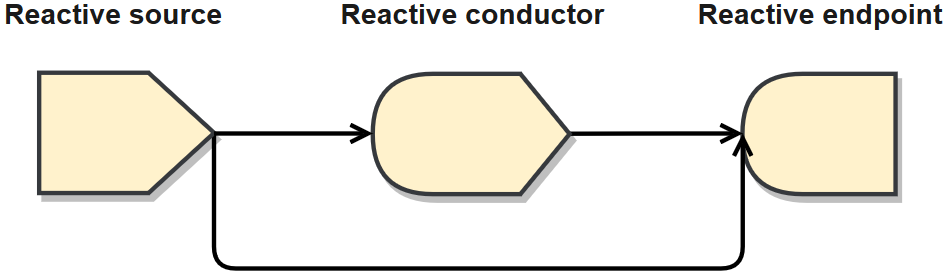
\includegraphics[width=0.7\linewidth]{Imagens/reactive}
	\caption{Representation of reactive programming objects in a Shiny application.}
	\label{reactive}
\end{figure}

The reactive source typically consists in the user input through a browser interface (e.g. selecting an item, typing input). A reactive endpoint is usually something that appears in the user's browser window, such as a plot or a table of values. A reactive source can be connected to multiple endpoints, and vice versa. Most simple examples use just these two components, wiring up sources directly to endpoints. However, it is also possible to put reactive components between the sources and endpoints, namely reactive conductors. These can be useful for encapsulating slow or computationally expensive operations, making sure code does not run more times than the absolutely necessary.

Other R libraries were also used. These include:
%the \textit{shinydashboard} library that allows the construction of a shiny application with a typical dashboard appearance; \textit{shinyBS} which adds additional Twitter Bootstrap components to Shiny including, for instance, modal windows; \textit{shinyjs} that allows to perform common useful JavaScript operations in Shiny apps like hiding, reseting or disabling elements; the \textit{DT} library that allows data objects in R to be rendered as HTML tables; \textit{RMySQL} library which is a database interface to MySQL; \textit{bcrypt} library for string encryption (used for the authentication system); the \textit{GGally} which is an extension of the graphics package \textit{ggplot2}; \textit{shinyWidgets} library that adds better looking custom inputs widgets to shiny applications; and the \textit{colourpicker} library that has a colour picker that can be used as an input in a shiny application, useful for interactively changing the color of some plots, for instance.

\begin{itemize}
	\item \textit{\textbf{shinydashboard}}: allows the construction of a shiny application with a typical dashboard appearance;
	\item \textit{\textbf{shinyBS}}: adds additional Twitter Bootstrap components to Shiny including, for instance, modal windows;
	\item \textit{\textbf{shinyjs}}: allows to perform common useful JavaScript operations in Shiny apps like hiding, reseting or disabling elements;
	\item \textit{\textbf{DT}}: allows data objects in R to be rendered as HTML tables;
	\item \textit{\textbf{RMySQL}}: a database interface to MySQL;
	\item \textit{\textbf{bcrypt}}: for string encryption (used for the authentication system);
	\item \textit{\textbf{GGally}}:	an extension of the graphics package \textit{ggplot2};
	\item \textit{\textbf{shinyWidgets}}: adds better looking custom inputs widgets to shiny applications;	
	\item \textit{\textbf{colourpicker}}: has a colour picker that can be used as an input in a shiny application, useful for interactively changing the color of some plots, for instance.
\end{itemize}

More importantly, the \textit{specmine} package was used, providing a set of methods for me\-ta\-bo\-lo\-mics data analysis, including data loading in different formats, pre-processing, metabolite identification, univariate and multivariate data analysis, machine learning and feature selection. The package functionalities will be introduced in detail in the next section, given its importance for this work.

The \gls{ide} chosen to develop the R scripts and build the platform was RStudio (\href{https://www.rstudio.com/}{\nolinkurl{https://www.rstudio.com/}}). It is written in the C++ programming language, having an intuitive interface with many usefull tools, making it easier to work with R. RStudio is a free software that has many features, including a console, syntax-highlighting editor that supports direct code execution, as well as tools for plotting, history, debugging and workspace management. 

Reports with the analysis results generated on the platform were made using the RStudio plug-in named R Markdown (\href{http://rmarkdown.rstudio.com/}{\nolinkurl{http://rmarkdown.rstudio.com/}}). R Markdown uses markdown syntax (\href{https://daringfireball.net/projects/markdown/}{\nolinkurl{https://daringfireball.net/projects/markdown/}}) coupled with R code chunks that are run, displaying the code's output in the generated report. The report is generated using the \textit{knitr} package (\href{https://yihui.name/knitr/}{\nolinkurl{https://yihui.name/knitr/}}), the engine for dynamic report generation with R, and it can be in the form of a HTML, PDF or Microsoft Word document. 

The database for project, dataset and user management was built using the open-source \gls{rdbms} MySQL (\href{https://www.mysql.com/}{\nolinkurl{https://www.mysql.com/}}). It is written in C and C++, being a fast, stable and multi-user, multi-threaded \gls{sql} database server. \gls{sql} consists of a data definition, manipulation and control language. It is a special-purpose domain-specific language used in programming and designed for stream processing or managing data held in a \gls{rdbms}. The scope of \gls{sql} includes data insert, query, update and delete, schema creation and modification, and data access control. 




	
	
\section{Specmine, an R package for metabolomics data analysis} \label{specmine_chapter}

As discussed in \autoref{met_tools}, most freely available tools are limited to specific types of metabolomics or spectral data and some offer a limited portfolio of data analysis tools for the construction of analysis pipelines. 

To address this problem, the R package \textit{specmine} was made available \citep{costa2016r}. It was developed under the R environment which is a free development environment for data manipulation, scientific and statistical computing and graphical visualization. \textit{Specmine} provides a set of methods for metabolomics and spectral data analysis, including data loading in various formats, data pre-processing, metabolite identification, univariate and multivariate data analysis, machine learning and also feature selection. 

The implemented methods allow for the analysis of metabolomics and spectral data, including \gls{gcms}, \gls{lcms}, \gls{nmr}, \gls{ir} and \gls{uv} data, integrating many available functions provided by other metabolomics oriented R packages and also more general-purpose data analysis R functions. Some of \textit{specmine} package dependencies include:

\begin{itemize}
	\item \textit{\textbf{hyperSpec}}: facilitates hyperspectral data sets handling (i.e. spatially or time-resolved spectra, which may consist of any data that is recorded over a discretized variable);
	\item \textit{\textbf{ChemoSpec}}: a collection of functions for top-down exploratory data analysis of spectral data obtained via \gls{nmr}, \gls{ir} or Raman spectroscopy;
	\item \textit{\textbf{rgl}}: provides medium to high level functions for 3D interactive graphics;
	\item \textit{\textbf{ggplot2}}: a system for 'declaratively' creating graphics, based on "The Grammar of Graphics";
	\item \textit{\textbf{caret}}: miscellaneous functions for training and plotting classification and regression models.
\end{itemize}

Besides providing a tool that covers the main metabolomics and spectral data types, \textit{specmine} also addresses a full range of tasks in data analysis, allowing for the creation of flexible and powerful analysis pipelines for specific case studies, providing abundant graphical visualization of the results. \autoref{specmine} shows the modules present in this package. Since metabolite identification is not usually the goal in a metabolic fingerprinting approach, which is emphasized throughout this dissertation, the metabolite identification module won't be discussed here.

\begin{figure}[!htb]
	\centering
	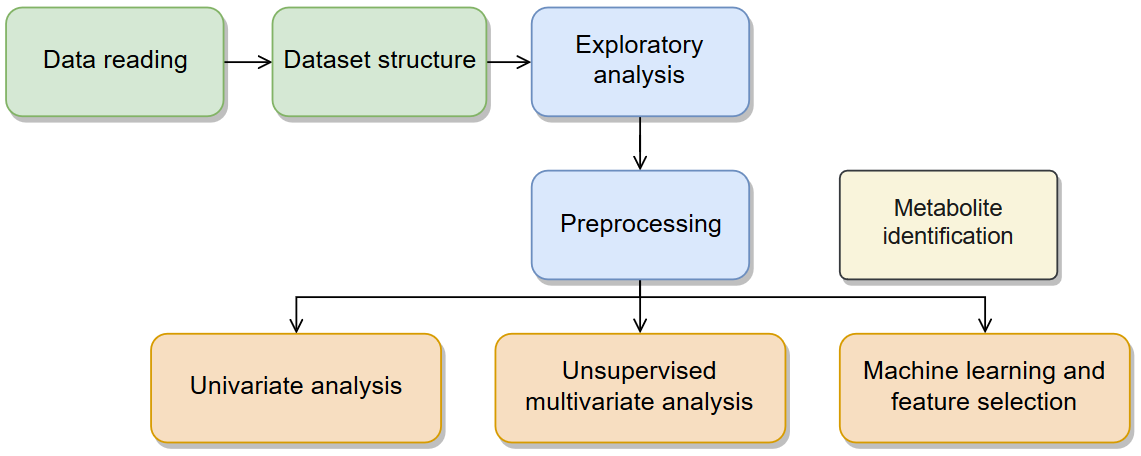
\includegraphics[width=0.85\linewidth]{Imagens/specmine}
	\caption{Modules in the \textit{specmine} package. Adapted from \cite{costa2016r}.}
	\label{specmine}
\end{figure}

\subsection{Data reading and dataset structure}

\textit{Specmine} supports a number of different file formats, including comma (or tab) separated values (CSV or TSV) files, (J)DX spectra files, NetCDF, mzDATA and mzXMLMS data. The metadata file can be given in the CSV/TSV format. Data can also be loaded as a peaks list, which are converted into a dataset using peak alignment functions. 

The structure of the dataset used in this package is independent of the data type and source and consists in an R list with the following fields: description of the dataset, the type of data, the data matrix, the metadata data frame and the labels for the x and y-axis. A graphical representation of the dataset structure is represented in \autoref{datas_tructure}.


\begin{figure}[!htb]
	\centering
	\includegraphics[width=0.9\linewidth]{Imagens/data_structure}
	\caption{Representation of the dataset structure in \textit{specmine}. Adapted from \cite{costa2016r}.}
	\label{datas_tructure}
\end{figure}

A list of all \textit{specmine} functions regarding data reading and dataset structure is shown in \autoref{specmine_functions_data_reading}.

\begin{scriptsize}
	\begin{longtable}{|m{4.3cm}|m{10cm}|}
		%FIRST HEADER------
		\caption{\textit{Specmine} package functions regarding data reading and dataset structure} 
		\label{specmine_functions_data_reading} \\
		\rowcolor{airforceblue}
		\htab{Function name} & \htab{Description} \\
		\hline
		\endfirsthead
		
		%SECOND HEADER------
		\caption[]{\textit{Specmine} package functions regarding data reading and dataset structure. (Continued)} \\
		\rowcolor{airforceblue}
		\htab{Function name} & \htab{Description} \\
		\hline
		\endhead
		
		%TABLE--------------
		
		\hline
		check\_dataset & Check if the dataset is valid and if not give the proper error message. \\
		
		\hline
		convert\_from\_chemospec & Convert the dataset in the ChemoSpec format to a dataset of this package. \\
		
		\hline
		convert\_from\_hyperspec & Convert the dataset in the hyperspec format to a dataset of this package. \\
		
		\hline
		convert\_to\_hyperspec & Convert a dataset to an hyperspec object. \\
		
		\hline
		create\_dataset & Create a dataset from existing objects. \\
		
		\hline
		dataset\_from\_peaks & Converts a peak list to a dataset. \\
		
		\hline
		is\_spectra & Check if the dataset is from spectral data where x.values are numeric. \\
		
		\hline
		read\_csvs\_folder & Reads multiple CSV files in a given folder. \\
		
		\hline
		read\_dataset\_csv & Reads the data from a CSV file and creates the dataset. \\
		
		\hline
		read\_dataset\_dx & Reads the data from the (J)DX files and creates the dataset. \\
		
		\hline
		read\_dataset\_spc & Reads the data from the SPC files and creates the dataset. \\
		
		\hline
		read\_data\_csv & Reads the data from the CSV file. \\
		
		\hline
		read\_data\_dx & Reads the data from the (J)DX files. \\
		
		\hline
		read\_data\_spc & Reads the data from the SPC files. \\
		
		\hline
		read\_metadata & Read the metadata from a file. \\
		
		\hline
		read\_ms\_spectra & Read the data from the MS files and creates the dataset. \\
		
		\hline
		read\_multiple\_csvs & Reads multiple CSVs, each one with a sample. \\
		
		\hline
		
	\end{longtable}
\end{scriptsize}

\subsection{Exploratory analysis and data pre-processing}

\textit{Specmine} includes functions that allow to calculate global statistics and visualize the data in a graphical way. The package can calculate the main descriptive statistics over the data matrix of a dataset for both variables and samples, having functions that can be applied over the entire dataset or to a subset of samples or variables. Graphical visualization of the data is done for instance in the form of boxplots, which allows to see the distribution of values for a set of variables. The package also provides functions for spectra plotting, where the variables are represented by numerical values. Visualization functions rely on both ggplot2 and the base graphics system of R.

Preprocessing methods are also provided for the different types of data. They include methods for extracting relevant parts of a dataset, namely subsets of samples, data and metadata variables. Spectral pre-processing methods include functions for shifting correction, multiplicative scatter correction, first derivative, baseline, offset and background corrections. Some methods for smoothing interpolation are also available, including bin or loess smoothing, as well as Savitzky-Golay filters. Missing values can be treated by either removing samples and/or variables that have a number of missing values above a given threshold or replaced using a variety of different methods. 

Specmine also includes functions for data normalization, which can be done by sum, median, a reference sample or feature, for data transformation using cubic root and logarithmic methods, and scaling using auto, range and pareto methods. The package also provides flat pattern filters with distinct metrics and parameters that allow to remove variables with low variance. The various \textit{specmine} functions for data exploratory analysis and pre-processing are listed in \autoref{specmine_functions_prepocessing}.

\begin{scriptsize}
	\begin{longtable}{|m{4.3cm}|m{11cm}|}
		%FIRST HEADER------
		\caption{\textit{Specmine} package functions for data exploratory analysis and pre-processing.} 
		\label{specmine_functions_prepocessing} \\
		\rowcolor{airforceblue}
		\htab{Function name} & \htab{Description} \\
		\hline
		\endfirsthead
		
		%SECOND HEADER------
		\caption[]{\textit{Specmine} package functions for data exploratory analysis and pre-processing. (Continued)} \\
		\rowcolor{airforceblue}
		\htab{Function name} & \htab{Description} \\
		\hline
		\endhead
		
		%TABLE--------------
		
		\hline
		absorbance\_to\_transmittance & Converts absorbance values to transmittance values. \\
		
		\hline
		aggregate\_samples & Aggregate samples according to an aggregate function like mean, median, etc. \\
		
		\hline
		apply\_by\_group & Apply a function to samples from a given metadata's group. \\
		
		\hline
		apply\_by\_groups & Apply a function to samples from a metadata's variable. \\
		
		\hline
		apply\_by\_sample & Applies a function to the values of each sample. \\
		
		\hline
		apply\_by\_variable & Applies a function to the values of each variable. \\
		
		\hline
		background\_correction & Perform background correction on the spectra. \\
		
		\hline
		baseline\_correction & Performs baseline correction on the dataset. \\
		
		\hline
		boxplot\_variables & Boxplot of each variable of the dataset. \\
		
		\hline
		boxplot\_vars\_factor & Boxplot of variables with metadata's variable factors from the dataset. \\
		
		\hline
		compare\_regions\_by\_sample & Compare two regions of a dataset by samples. \\
		
		\hline
		convert\_to\_factor & Convert a metadata's variable to factor. \\
		
		\hline
		count\_missing\_values & Counts the missing values on the dataset. \\
		
		\hline
		count\_missing\_values\_per\_sample & Counts the missing values on each sample of the dataset. \\
		
		\hline
		count\_missing\_values\_per\_variable & Counts the missing values on each variable of the dataset. \\
		
		\hline
		cubic\_root\_transform & Performs cubic root transformation on the data matrix. \\
		
		\hline
		data\_correction & Perform spectra corrections with 3 different methods. \\
		
		\hline
		find\_equal\_samples & Finds samples that have the same peak values - $ x $ and $ y $ (equal data frames). \\
		
		\hline
		first\_derivative & Calculates the first derivative of the data. \\
		
		\hline
		get\_data & Get the data matrix from dataset. \\
		
		\hline
		get\_data\_as\_df & Get the data matrix from the dataset as a data frame. \\
		
		\hline
		get\_data\_value & Get a data value given the x-axis labels and the sample. \\
		
		\hline
		get\_data\_values & Gets the values of all samples in the dataset given a set of x axis names or indexes. \\
		
		\hline
		get\_metadata & Get the metadata from the dataset. \\
		
		\hline
		get\_metadata\_value & Get the metadata value. \\
		
		\hline
		get\_metadata\_var & Get the values of a metadata variable from the dataset. \\
		
		\hline
		get\_peak\_values & Gets the peak values from a data frame of samples’ peaks. \\
		
		\hline
		get\_samples\_names\_dx & Function to get the names of the DX files from a folder. \\
		
		\hline
		get\_samples\_names\_spc & Function to get the names of the SPC files from a folder. \\
		
		\hline
		get\_sample\_names & Get the sample names from the dataset. \\
		
		\hline
		get\_type & Get the type of the data from the dataset. \\
		
		\hline
		get\_value\_label & Get the value label from the dataset. \\
		
		\hline
		get\_x\_label & Get the x-axis label from the dataset. \\
		
		\hline
		get\_x\_values\_as\_num & Get the x-axis values from the dataset as numbers. \\
		
		\hline
		get\_x\_values\_as\_text & Get the x-axis values from the dataset as text. \\
		
		\hline
		group\_peaks & Group peaks with peak alignment. \\
		
		\hline
		impute\_nas\_knn & Impute missing values with \gls{knn}. \\
		
		\hline
		impute\_nas\_linapprox & Impute missing values with linear approximation. \\
		
		\hline
		impute\_nas\_mean & Impute missing values with mean. \\
		
		\hline
		impute\_nas\_median & Impute missing values with median. \\
		
		\hline
		impute\_nas\_value & Impute missing values with value replacement. \\
		
		\hline
		indexes\_to\_xvalue\_interval & Returns x-values corresponding to a vector of indexes (only to numerical values - spectra). \\
		
		\hline
		log\_transform & Performs logarithmic transformation on the data matrix. \\
		
		\hline
		low\_level\_fusion & Low level fusion method for integrate different datasets (only samples with the same name on all
		datasets will be merged). \\
		
		\hline
		mean\_centering & Performs mean centering on the dataset. \\
		
		\hline
		merge\_datasets & Merges two datasets with the same variables and metadata’s variables. \\
		
		\hline
		merge\_data\_metadata & Merges the data and metadata from the dataset into a single data.frame. \\
		
		\hline
		metadata\_as\_variables & Use one or more metadata variables as variables. \\
		
		\hline
		missingvalues\_imputation & Treats the missing values of a dataset according to a specific method. \\
		
		\hline
		msc\_correction & Perform multiplicative scatter correction on the spectra. \\
		
		\hline
		multiplot & Multiplot from \textit{ggplot2} package. \\
		
		\hline
		normalize & Normalize the data from the dataset with a specific method. \\
		
		\hline
		normalize\_samples & Normalize the data from a datamatrix with a specific method. \\
		
		\hline
		num\_samples & Get the number of samples from a dataset. \\
		
		\hline
		num\_x\_values & Get the number of x-axis values. \\
		
		\hline
		offset\_correction & Perform offset correction on the data. \\
		
		\hline
		peaks\_per\_sample & Counts number of peaks in a sample (given its index). \\
		
		\hline
		peaks\_per\_samples & Calculates the number of peaks on each sample. \\
		
		\hline
		plotvar\_twofactor & Plot variable distribution on two factors from the dataset. \\
		
		\hline
		plot\_spectra & Plot spectra from dataset. \\
		
		\hline
		plot\_spectra\_simple & Plot spectra from dataset (simple version). \\
		
		\hline
		remove\_data & Remove data from the dataset. \\
		
		\hline
		remove\_data\_variables & Remove data variables from the dataset. \\
		
		\hline
		remove\_metadata\_variables & Remove metadata's variables from the dataset. \\
		
		\hline
		remove\_peaks\_interval & Removes peaks from a given interval. \\
		
		\hline
		remove\_peaks\_interval\_sample\_list & Removes peaks on a sample list given a peak interval. \\
		
		\hline
		remove\_samples & Remove samples from the dataset. \\
		
		\hline
		remove\_samples\_by\_nas & Remove samples from the dataset by the number of NAs. \\
		
		\hline
		remove\_samples\_by\_na\_metadata & Remove samples from the dataset with the metadata's variable value with NAs. \\
		
		\hline
		remove\_variables\_by\_nas & Remove variables from the dataset by the number of NAs. \\
		
		\hline
		remove\_x\_values\_by\_interval & Remove an interval of x-values from the dataset. \\
		
		\hline
		replace\_data\_value & Replace a data value for a new value on the dataset. \\
		
		\hline
		replace\_metadata\_value & Replace a metadata’s variable value of a sample. \\
		
		\hline
		savitzky\_golay & Smoothing and derivative of the data using Savitzky-Golay. \\
		
		\hline
		scaling & Performs scaling according to a method. \\
		
		\hline
		scaling\_samples & Performs scaling according to a method. \\
		
		\hline
		set\_metadata & Updates the dataset’s metadata with a new one. \\
		
		\hline
		set\_sample\_names & Set new samples names to the dataset. \\
		
		\hline
		set\_value\_label & Set a new value label for the dataset. \\
		
		\hline
		set\_x\_label & Set a new x-label to the dataset. \\
		
		\hline
		set\_x\_values & Set new x-values to the dataset. \\
		
		\hline
		shift\_correction & Shifts the spectra according to a specific method. \\
		
		\hline
		smoothing\_interpolation & Performs smoothing interpolation according to a specific method. \\
		
		\hline
		snv\_dataset & Performs Standard Normal Variate on the dataset. \\
		
		\hline
		stats\_by\_sample & Get a summary of statistics of the samples. \\
		
		\hline
		stats\_by\_variable & Get a summary of statistics of the variables. \\
		
		\hline
		subset\_by\_samples\_and\_xvalues & Gets a subset of specific samples and x-values. \\
		
		\hline
		subset\_metadata & Subsets the metadata according to the specified metadata's variables. \\
		
		\hline
		subset\_random\_samples & Gets a subset of random samples from the dataset. \\
		
		\hline
		subset\_samples & Gets a subset of specific samples from the dataset. \\
		
		\hline
		subset\_samples\_by\_metadata\_values & Gets a subset of specific samples according to metadata’s values from the dataset. \\
		
		\hline
		subset\_x\_values & Gets a subset of specific x-values from the dataset. \\
		
		\hline
		subset\_x\_values\_by\_interval & Gets a subset of a specific interval of x-values. \\
		
		\hline
		sum\_dataset & Returns a summary with its main features. \\
		
		\hline
		transform\_data & Performs data transformation according to a method. \\
		
		\hline
		transmittance\_to\_absorbance & Converts transmittance values to absorbance values. \\
		
		\hline
		values\_per\_peak & Gets the number of values on each peak. \\
		
		\hline
		values\_per\_sample & Gets the number of values on each sample. \\
		
		\hline
		variables\_as\_metadata & Use one or more data variables as metadata variables. \\
		
		\hline
		xvalue\_interval\_to\_indexes & Returns indexes corresponding to an interval of x-values (only to numerical values - spectra). \\
		
		\hline
		x\_values\_to\_indexes & Returns the indexes corresponding to a vector of x-values (only to numerical values - spectra). \\
		
		\hline
		
	\end{longtable}
\end{scriptsize}


\subsection{Univariate and unsupervised multivariate analysis}

For univariate analysis, \textit{specmine} offers a set of functions that cover various analysis types such as t-tests, \gls{anova}, regression analysis, correlations and \gls{fc} calculation. The package offers one-way \gls{anova}, with the Tukey \gls{hsd} post hoc test, and also multifactorial \gls{anova}, with functions to summarize the main results, including p-values and the percentage of variation explained by the different factors. These p-values are already adjusted using the \gls{fdr} method. Non-parametric tests include the Kruskal-Wallis and Kolmogorov-Smirnov tests. 

For the linear regression analysis \textit{specmine} offers functions that summarize the coefficients for the different factors and interactions and respective p-values. The correlations between variables or samples can be computed and the resulting matrix visualized as a heatmap. For \gls{fc} analysis the package offers functions to calculate the fold changes of values considering two groups of samples, and the results can be visualized in both tabular and graphical forms, similarly to the t-tests results.
 
As for the unsupervised multivariate analysis \textit{specmine} provides functions to perform \gls{pca} using two methods: classical and robust, where the latter makes use of the grid search algorithm to compute the desired number of principal components. The results of \gls{pca} can be visualized through a variety of graphs, including scree plots, scores plots, biplots and pairs plots. 

The package also offers functions to perform k-means and hierarchical clustering methods. The distance method to use can be chosen as well as the method to use in the case of hierarchical clustering. K-means clustering results can be plotted in the form of a graph with the k clusters in different colors and hierarchical clustering results plotted as a dendogram. The various \textit{specmine} functions for univariate and unsupervised multivariate analysis are listed in \autoref{specmine_functions_analysis}.



\begin{scriptsize}
	\begin{longtable}{|m{4.3cm}|m{11cm}|}
		%FIRST HEADER------
		\caption{\textit{Specmine} package functions for univariate and unsupervised multivariate analysis.} 
		\label{specmine_functions_analysis} \\
		\rowcolor{airforceblue}
		\htab{Function name} & \htab{Description} \\
		\hline
		\endfirsthead
		
		%SECOND HEADER------
		\caption[]{\textit{Specmine} package functions for univariate and unsupervised multivariate analysis. (Continued)} \\
		\rowcolor{airforceblue}
		\htab{Function name} & \htab{Description} \\
		\hline
		\endhead
		
		%TABLE--------------
		
		\hline
		aov\_all\_vars & Perform analysis of variance of all variables in the dataset. \\
		
		\hline
		clustering & Perform cluster analysis on the dataset. \\
		
		\hline
		correlations\_dataset & Calculate the correlations of all variables or samples in the dataset. \\
		
		\hline
		correlations\_test & Performs correlations test to the whole dataset. \\
		
		\hline
		correlation\_test & Performs correlations test of two variables or samples from the dataset. \\
		
		\hline
		dendrogram\_plot & Plot dendrogram of hierarchical clustering results. \\
		
		\hline
		dendrogram\_plot\_col & Plot dendrogram of hierarchical clustering results with different colors. \\
		
		\hline
		fold\_change & Perform \acrlong{fc} analysis on the dataset. \\
		
		\hline
		fold\_change\_var & \acrlong{fc} applied on two variables. Instead of having the difference of the variables on two groups, we have the difference of the groups on two variables. \\
		
		\hline
		heatmap\_correlations & Plots a heatmap with the correlations. \\
		
		\hline
		hierarchical\_clustering & Perform \acrlong{hca} on the dataset. \\
		
		\hline
		kmeans\_clustering & Perform k-means clustering analysis on the dataset. \\
		
		\hline
		kmeans\_plot & Plot for each formed cluster, in grey the values of all samples of that cluster and in blue the median
		of that samples. \\
		
		\hline
		kmeans\_result\_df & Show for each cluster from kmeans analysis the sample names belonging to them. \\
		
		\hline
		kruskalTest\_dataset & Run Kruskal-Wallis Tests for each row of the data from the dataset. \\
		
		\hline
		ksTest\_dataset & Run Kolmogorov-Smirnov Tests for each row of the data from the dataset. \\
		
		\hline
		linregression\_onevar & Performs linear regression on one variable of the dataset. \\
		
		\hline
		linreg\_all\_vars & Performs linear regression analysis over the dataset. \\
		
		\hline
		linreg\_coef\_table & Gets a data frame with the coefficient values. \\
		
		\hline
		linreg\_pvalue\_table & Gets the p-values table from the linear regression analysis. \\
		
		\hline
		linreg\_rsquared & Gets the linear regression r-squared values. \\
		
		\hline
		multifactor\_aov\_all\_vars & Perform multi-factor \gls{anova} on all variables with the selected metadata variables. \\
		
		\hline
		multifactor\_aov\_pvalues\_table & Gets the p-values table from the multifactor \gls{anova} results. \\
		
		\hline
		multifactor\_aov\_varexp\_table & Gets the variability explained table from the multifactor \gls{anova} results. \\
		
		\hline
		pca\_analysis\_dataset & Performs a classical \gls{pca} over the dataset. \\
		
		\hline
		pca\_biplot & Shows a \gls{pca} biplot. \\
		
		\hline
		pca\_biplot3D & Shows a interactive 3D \gls{pca} biplot. \\
		
		\hline 
		pca\_importance & Gets the importance from the PCs. \\
		
		\hline
		pca\_kmeans\_plot2D & Groups the points with the clusters given by k-means in a 2D \gls{pca} scores plot. \\
		
		\hline
		pca\_kmeans\_plot3D & Groups the points with the clusters given by k-means in a interactive 3D \gls{pca} scores plot. \\
		
		\hline
		pca\_pairs\_kmeans\_plot & Groups the points with the clusters from k-means in a \gls{pca} pairs plot. \\
		
		\hline
		pca\_pairs\_plot & Shows a \gls{pca} pairs plot. \\
		
		\hline
		pca\_plot\_3d & 3D plot from 3 components. \\
		
		\hline
		pca\_robust & Performs a robust \gls{pca} analysis. \\
		
		\hline
		pca\_scoresplot2D & Shows a 2D \gls{pca} scores plot of two principal components. \\
		
		\hline
		pca\_scoresplot3D & Shows a 3D \gls{pca} scores plot of three principal components. \\
		
		\hline
		pca\_scoresplot3D\_rgl & Shows a interactive 3D \gls{pca} scores plot of three principal components. \\
		
		\hline
		pca\_screeplot & \gls{pca} scree plot with the proportion and cumulative variance of the PCs. \\
		
		\hline
		plot\_anova & Function for plotting the results from \gls{anova}.
		Usage \\
		
		\hline
		plot\_fold\_change & Function for plotting the results from \gls{fc}. \\
		
		\hline
		plot\_kruskaltest & Function for plotting the results from Kruskal-Wallis tests. \\
		
		\hline
		plot\_kstest & Function for plotting the results from Kolmogorov-Smirnov tests. \\
		
		\hline
		plot\_regression\_coefs\_pvalues & Plots the linear regression coefficient and the p-values. \\
		
		\hline
		plot\_ttests & Function for plotting the results from t-tests. \\
		
		\hline
		tTests\_dataset & Run t-Tests for each row of the data from the dataset. \\
		
		\hline
		volcano\_plot\_fc\_tt & Volcano plot to intersect the results from t-tests and \gls{fc}. \\
		
		\hline
		
	\end{longtable}
\end{scriptsize}


\subsection{Machine learning and feature selection}

For machine learning, the package offers a number of functions to train, use and evaluate the different methods, covering both classification and regression approaches. It also includes validation methods to estimate the error metrics, including k-fold cross-validation, leave-one-out cross-validation and resampling methods, among others. The error metrics available include accuracy, \gls{auc} and kappa statistic for classification, and \gls{rmse} and the coefficient of determination ($ R^{2} $) for regression. Functions to optimize model parameters (e.g. hidden nodes in a neural network) by testing and evaluating different values, according to the selected validation method and error metrics, are also available. This model optimization process gives the best model obtained and its performance, the variables’ importance, the results of all tested combinations of parameters, the confusion matrices (in the case of classification), among other statistics. The resulting trained models can then be used for new data prediction.

Feature selection methods provided by \textit{specmine} include both filter and wrapper methods, which can be combined with the machine learning methods. The package includes the most commonly used wrapper method \gls{rfe}, which tests different subsets of features, iteratively reducing the number of features and verifying which configuration provides the best performance. The various \textit{specmine} functions for machine learning and feature selection are listed in \autoref{specmine_functions_machine_learning}.


\begin{scriptsize}
	\begin{longtable}{|m{4.3cm}|m{11cm}|}
		%FIRST HEADER------
		\caption{\textit{Specmine} package functions for machine learning and feature selection.} 
		\label{specmine_functions_machine_learning} \\
		\rowcolor{airforceblue}
		\htab{Function name} & \htab{Description} \\
		\hline
		\endfirsthead
		
		%SECOND HEADER------
		\caption[]{\textit{Specmine} package functions for machine learning and feature selection. (Continued)} \\
		\rowcolor{airforceblue}
		\htab{Function name} & \htab{Description} \\
		\hline
		\endhead
		
		%TABLE--------------
		
		\hline
		feature\_selection & Perform feature selection on the dataset. \\
		
		\hline
		filter\_feature\_selection & Perform selection by filter using univariate filters, from \textit{caret}'s package. \\
		
		\hline
		flat\_pattern\_filter & Performs a flat pattern filter over the dataset. \\
		
		\hline
		multiClassSummary & Summary function for caret to compute \acrshort{auc}. \\
		
		\hline
		predict\_samples & Predict new samples. \\
		
		\hline
		recursive\_feature\_elimination & Perform \acrlong{rfe} on the dataset using \textit{caret}'s package. \\
		
		\hline
		summary\_var\_importance & Summary of variables importance of the models. \\
		
		\hline
		train\_and\_predict & Train a model and predict new unlabeled samples with that model. \\
		
		\hline
		train\_classifier & Train a specific classifier. \\
		
		\hline
		train\_models\_performance & Train various models. \\
		
		\hline
		
	\end{longtable}
\end{scriptsize}




%\definecolor{moonstoneblue}{rgb}{0.64, 0.76, 0.68}
%
%\begin{scriptsize}
%	\begin{longtable}{|m{4.3cm}|m{11cm}|}
%		%FIRST HEADER------
%		\caption{\textit{Specmine} package functions.} 
%		\label{specmine_functions} \\
%		\rowcolor{airforceblue}
%		\htab{Function name} & \htab{Description} \\
%		\hline
%		\endfirsthead
%		
%		%SECOND HEADER------
%		\caption[]{\textit{Specmine} package functions. (Continued)} \\
%		\rowcolor{airforceblue}
%		\htab{Function name} & \htab{Description} \\
%		\hline
%		\endhead
%		
%		%TABLE--------------
%		
%		\hline
%		\rowcolor{moonstoneblue}
%		\multicolumn{2}{|l|}{\htab{Data reading and dataset structure}} \\ 
%		
%		 \hline
%		check\_dataset & Check if the dataset is valid and if not give the proper error message. \\
%								
%		\hline
%		convert\_from\_chemospec & Convert the dataset in the ChemoSpec format to a dataset of this package. \\
%		
%		\hline
%		convert\_from\_hyperspec & Convert the dataset in the hyperspec format to a dataset of this package. \\
%		
%		\hline
%		convert\_to\_hyperspec & Convert a dataset to an hyperspec object. \\
%						
%		\hline
%		create\_dataset & Create a dataset from existing objects \\
%		
%		\hline
%		dataset\_from\_peaks & Converts a peak list to a dataset. \\
%		
%		\hline
%		is\_spectra & Check if the dataset is from spectral data where x.values are numeric. \\
%		
%		\hline
%		read\_csvs\_folder & Reads multiple CSV files in a given folder. \\
%		
%		\hline
%		read\_dataset\_csv & Reads the data from a CSV file and creates the dataset. \\
%		
%		\hline
%		read\_dataset\_dx & Reads the data from the (J)DX files and creates the dataset. \\
%		
%		\hline
%		read\_dataset\_spc & Reads the data from the SPC files and creates the dataset. \\
%		
%		\hline
%		read\_data\_csv & Reads the data from the CSV file. \\
%		
%		\hline
%		read\_data\_dx & Reads the data from the (J)DX files. \\
%		
%		\hline
%		read\_data\_spc & Reads the data from the SPC files. \\
%		
%		\hline
%		read\_metadata & Read the metadata from a file. \\
%		
%		\hline
%		read\_ms\_spectra & Read the data from the MS files and creates the dataset. \\
%		
%		\hline
%		read\_multiple\_csvs & Reads multiple CSVs, each one with a sample. \\
%		
%		
%		% EXPLORATORY ANALYSIS AND PREPROCESSING
%		\hline
%		\rowcolor{moonstoneblue}
%		\multicolumn{2}{|l|}{\htab{Exploratory analysis and data pre-processing}} \\ 
%		
%		\hline
%		absorbance\_to\_transmittance & Converts absorbance values to transmittance values. \\
%		
%		\hline
%		aggregate\_samples & Aggregate samples according to an aggregate function like mean, median, etc. \\
%		
%		\hline
%		apply\_by\_group & Apply a function to samples from a given metadata's group. \\
%		
%		\hline
%		apply\_by\_groups & Apply a function to samples from a metadata's variable. \\
%		
%		\hline
%		apply\_by\_sample & Applies a function to the values of each sample \\
%								
%		\hline
%		apply\_by\_variable & Applies a function to the values of each variable \\
%		
%		\hline
%		background\_correction & Perform background correction on the spectra. \\
%		
%		\hline
%		baseline\_correction & Performs baseline correction on the dataset. \\
%		
%		\hline
%		boxplot\_variables & Boxplot of each variable of the dataset. \\
%		
%		\hline
%		boxplot\_vars\_factor & Boxplot of variables with metadata's variable factors from the dataset. \\
%		
%		\hline
%		compare\_regions\_by\_sample & Compare two regions of a dataset by samples. \\
%		
%		\hline
%		convert\_to\_factor & Convert a metadata's variable to factor. \\
%								
%		\hline
%		count\_missing\_values & Counts the missing values on the dataset. \\
%		
%		\hline
%		count\_missing\_values\_per\_sample & Counts the missing values on each sample of the dataset. \\
%		
%		\hline
%		count\_missing\_values\_per\_variable & Counts the missing values on each variable of the dataset. \\
%		
%		\hline
%		cubic\_root\_transform & Performs cubic root transformation on the data matrix. \\
%		
%		\hline
%		data\_correction & Perform spectra corrections with 3 different methods. \\
%		
%		\hline
%		\rowcolor{moonstoneblue}
%		\multicolumn{2}{|l|}{\htab{Exploratory analysis and data pre-processing}} \\ 
%		
%		\hline
%		find\_equal\_samples & Finds samples that have the same peak values - $ x $ and $ y $ (equal data frames) \\
%		
%		\hline
%		first\_derivative & Calculates the first derivative of the data. \\
%		
%		\hline
%		get\_data & Get the data matrix from dataset \\
%		
%		\hline
%		get\_data\_as\_df & Get the data matrix from the dataset as a data frame. \\
%		
%		\hline
%		get\_data\_value & Get a data value given the x-axis labels and the sample \\
%		
%		\hline
%		get\_data\_values & Gets the values of all samples in the dataset given a set of x axis names or indexes. \\
%		
%		\hline
%		get\_metadata & Get the metadata from the dataset \\
%		
%		\hline
%		get\_metadata\_value & Get the metadata value \\
%		
%		\hline
%		get\_metadata\_var & Get the values of a metadata variable from the dataset. \\
%		
%		\hline
%		get\_peak\_values & Gets the peak values from a data frame of samples’ peaks. \\
%								
%		\hline
%		get\_samples\_names\_dx & Function to get the names of the DX files from a folder. \\
%		
%		\hline
%		get\_samples\_names\_spc & Function to get the names of the SPC files from a folder. \\
%		
%		\hline
%		get\_sample\_names & Get the sample names from the dataset. \\
%								
%		\hline
%		get\_type & Get the type of the data from the dataset \\
%		
%		\hline
%		get\_value\_label & Get the value label from the dataset \\
%		
%		\hline
%		get\_x\_label & Get the x-axis label from the dataset. \\
%		
%		\hline
%		get\_x\_values\_as\_num & Get the x-axis values from the dataset as numbers. \\
%		
%		\hline
%		get\_x\_values\_as\_text & Get the x-axis values from the dataset as text. \\
%		
%		\hline
%		group\_peaks & Group peaks with peak alignment. \\
%		
%		\hline
%		impute\_nas\_knn & Impute missing values with KNN \\
%		
%		\hline
%		impute\_nas\_linapprox & Impute missing values with linear approximation. \\
%		
%		\hline
%		impute\_nas\_mean & Impute missing values with mean \\
%		
%		\hline
%		impute\_nas\_median & Impute missing values with median \\
%		
%		\hline
%		impute\_nas\_value & Impute missing values with value replacement. \\
%		
%		\hline
%		indexes\_to\_xvalue\_interval & Returns x-values corresponding to a vector of indexes (only to numerical values - spectra) \\
%		
%		\hline
%		log\_transform & Performs logarithmic transformation on the data matrix. \\
%								
%		\hline
%		low\_level\_fusion & Low level fusion method for integrate different datasets (only samples with the same name on all
%		datasets will be merged) \\
%		
%		\hline
%		mean\_centering & Performs mean centering on the dataset. \\
%		
%		\hline
%		merge\_datasets & Merges two datasets with the same variables and metadata’s variables. \\
%		
%		\hline
%		merge\_data\_metadata & Merges the data and metadata from the dataset into a single data.frame. \\
%		
%		\hline
%		metadata\_as\_variables & Use one or more metadata variables as variables. \\
%		
%		\hline
%		missingvalues\_imputation & Treats the missing values of a dataset according to a specific method. \\
%		
%		\hline
%		msc\_correction & Perform multiplicative scatter correction on the spectra. \\
%		
%		\hline
%		multiplot & Multiplot from \textit{ggplot2} package \\
%		
%		\hline
%		normalize & Normalize the data from the dataset with a specific method. \\
%		
%		\hline
%		normalize\_samples & Normalize the data from a datamatrix with a specific method. \\
%		
%		\hline
%		num\_samples & Get the number of samples from a dataset. \\
%		
%		\hline
%		num\_x\_values & Get the number of x-axis values. \\
%		
%		\hline
%		offset\_correction & Perform offset correction on the data. \\
%		
%		\hline
%		peaks\_per\_sample & Counts number of peaks in a sample (given its index). \\
%		
%		\hline
%	 	peaks\_per\_samples & Calculates the number of peaks on each sample. \\
%		
%		\hline
%		plotvar\_twofactor & Plot variable distribution on two factors from the dataset. \\
%		
%		\hline
%		plot\_spectra & Plot spectra from dataset. \\
%		
%		\hline
%		plot\_spectra\_simple & Plot spectra from dataset (simple version). \\
%		
%		\hline
%		remove\_data & Remove data from the dataset. \\
%		
%		\hline
%		remove\_data\_variables & Remove data variables from the dataset. \\
%		
%		\hline
%		\rowcolor{moonstoneblue}
%		\multicolumn{2}{|l|}{\htab{Exploratory analysis and data pre-processing}} \\ 
%		
%		\hline
%		remove\_metadata\_variables & Remove metadata's variables from the dataset \\
%		
%		\hline
%		remove\_peaks\_interval & Removes peaks from a given interval. \\
%		
%		\hline
%	 	remove\_peaks\_interval\_sample\_list & Removes peaks on a sample list given a peak interval. \\
%		
%		\hline
%		remove\_samples & Remove samples from the dataset. \\
%		
%		\hline
%		remove\_samples\_by\_nas & Remove samples from the dataset by the number of NAs \\
%		
%		\hline
%		remove\_samples\_by\_na\_metadata & Remove samples from the dataset with the metadata's variable value with NAs. \\
%		
%		\hline
%		remove\_variables\_by\_nas & Remove variables from the dataset by the number of NAs \\
%		
%		\hline
%		remove\_x\_values\_by\_interval & Remove an interval of x-values from the dataset. \\
%		
%		\hline
%		replace\_data\_value & Replace a data value for a new value on the dataset. \\
%		
%		\hline
%		replace\_metadata\_value & Replace a metadata’s variable value of a sample. \\
%		
%		\hline
%		savitzky\_golay & Smoothing and derivative of the data using Savitzky-Golay. \\
%		
%		\hline
%		scaling & Performs scaling according to a method. \\
%		
%		\hline
%		scaling\_samples & Performs scaling according to a method. \\
%		
%		\hline
%		set\_metadata & Updates the dataset’s metadata with a new one. \\
%		
%		\hline
%		set\_sample\_names & Set new samples names to the dataset. \\
%		
%		\hline
%	 	set\_value\_label & Set a new value label for the dataset. \\
%		
%		\hline
%		set\_x\_label & Set a new x-label to the dataset. \\
%		
%		\hline
%		set\_x\_values & Set new x-values to the dataset \\
%		
%		\hline
%		shift\_correction & Shifts the spectra according to a specific method. \\
%		
%		\hline
%		smoothing\_interpolation & Performs smoothing interpolation according to a specific method. \\
%		
%		\hline
%		snv\_dataset & Performs Standard Normal Variate on the dataset. \\
%		
%		\hline
%		stats\_by\_sample & Get a summary of statistics of the samples. \\
%		
%		\hline
%		stats\_by\_variable & Get a summary of statistics of the variables. \\
%		
%		\hline
%		subset\_by\_samples\_and\_xvalues & Gets a subset of specific samples and x-values. \\
%		
%		\hline
%		subset\_metadata & Subsets the metadata according to the specified metadata's variables. \\
%		
%		\hline
%		subset\_random\_samples & Gets a subset of random samples from the dataset. \\
%		
%		\hline
%		subset\_samples & Gets a subset of specific samples from the dataset. \\
%		
%		\hline
%		subset\_samples\_by\_metadata\_values & Gets a subset of specific samples according to metadata’s values from the dataset. \\
%		
%		\hline
%		subset\_x\_values & Gets a subset of specific x-values from the dataset. \\
%		
%		\hline
%		subset\_x\_values\_by\_interval & Gets a subset of a specific interval of x-values. \\
%		
%		\hline
%		sum\_dataset & Returns a summary with its main features. \\
%		
%		\hline
%		transform\_data & Performs data transformation according to a method. \\
%		
%		\hline
%		transmittance\_to\_absorbance & Converts transmittance values to absorbance values. \\
%		
%		\hline
%		values\_per\_peak & Gets the number of values on each peak. \\
%		
%		\hline
%		values\_per\_sample & Gets the number of values on each sample. \\
%		
%		\hline
%		variables\_as\_metadata & Use one or more data variables as metadata variables. \\
%		
%		\hline
%		xvalue\_interval\_to\_indexes & Returns indexes corresponding to an interval of x-values (only to numerical values - spectra) \\
%		
%		\hline
%		x\_values\_to\_indexes & Returns the indexes corresponding to a vector of x-values (only to numerical values - spectra) \\
%	
%		% UNIVARIATE ANALYSIS
%		\hline
%		\rowcolor{moonstoneblue}
%		\multicolumn{2}{|l|}{\htab{Univariate and unsupervised multivariate analysis}} \\ 
%				
%		\hline
%		aov\_all\_vars & Perform analysis of variance of all variables in the dataset. \\
%		
%		\hline
%		clustering & Perform cluster analysis on the dataset. \\
%		
%		\hline
%		correlations\_dataset & Calculate the correlations of all variables or samples in the dataset. \\
%		
%		\hline
%	 	correlations\_test & Performs correlations test to the whole dataset. \\
%						
%		\hline
%		correlation\_test & Performs correlations test of two variables or samples from the dataset. \\
%		
%		\hline
%		dendrogram\_plot & Plot dendrogram of hierarchical clustering results. \\
%		
%		\hline
%		dendrogram\_plot\_col & Plot dendrogram of hierarchical clustering results with different colors \\
%		
%		\hline
%		\rowcolor{moonstoneblue}
%		\multicolumn{2}{|l|}{\htab{Univariate and unsupervised multivariate analysis}} \\ 
%		
%		\hline
%		fold\_change & Perform fold change analysis on the dataset. \\
%		
%		\hline
%		fold\_change\_var & Fold change applied on two variables. Instead of having the difference of the variables on two
%		groups, we have the difference of the groups on two variables. \\
%		
%		\hline
%		heatmap\_correlations & Plots a heatmap with the correlations. \\
%		
%		\hline
%		hierarchical\_clustering & Perform hierarchical clustering analysis on the dataset. \\
%		
%		\hline
%		kmeans\_clustering & Perform k-means clustering analysis on the dataset. \\
%		
%		\hline
%		kmeans\_plot & Plot for each formed cluster, in grey the values of all samples of that cluster and in blue the median
%		of that samples. \\
%		
%		\hline
%		kmeans\_result\_df & Show for each cluster from kmeans analysis the sample names belonging to them. \\
%		
%		\hline
%		kruskalTest\_dataset & Run Kruskal-Wallis Tests for each row of the data from the dataset. \\
%		
%		\hline
%		ksTest\_dataset & Run Kolmogorov-Smirnov Tests for each row of the data from the dataset. \\
%		
%		\hline
%	 	linregression\_onevar & Performs linear regression on one variable of the dataset. \\
%		
%		\hline
%	 	linreg\_all\_vars & Performs linear regression analysis over the dataset with the selected metadata’s variables. \\
%		
%		\hline
%		linreg\_coef\_table & Gets a data.frame with the coefficient values. \\
%							
%		\hline
%		linreg\_pvalue\_table & Gets the p-values table from the linear regression analysis. \\
%		
%		\hline
%		linreg\_rsquared & Gets the linear regression r-squared values. \\
%		
%		\hline
%		multifactor\_aov\_all\_vars & Perform multi-factor ANOVA on all variables with the selected metadata variables. \\
%		
%		\hline
%		multifactor\_aov\_pvalues\_table & Gets the p-values table from the multifactor ANOVA results. \\
%		
%		\hline
%		multifactor\_aov\_varexp\_table & Gets the variability explained table from the multifactor ANOVA results. \\
%		
%		\hline
%		pca\_analysis\_dataset & Performs a classical PCA analysis over the dataset. \\
%		
%		\hline
%		pca\_biplot & Shows a PCA biplot. \\
%		
%		\hline
%		pca\_biplot3D & Shows a interactive 3D PCA biplot. \\
%		
%		\hline 
%		pca\_importance & Gets the importance from the PCs. \\
%		
%		\hline
%		pca\_kmeans\_plot2D & Groups the points with the clusters given by k-means in a 2D PCA scores plot. \\
%		
%		\hline
%		pca\_kmeans\_plot3D & Groups the points with the clusters given by k-means in a interactive 3D PCA scores plot. \\
%		
%		\hline
%		pca\_pairs\_kmeans\_plot & Groups the points with the clusters from k-means in a PCA pairs plot. \\
%		
%		\hline
%		pca\_pairs\_plot & Shows a PCA pairs plot. \\
%		
%		\hline
%		pca\_plot\_3d & 3D plot from 3 components \\
%		
%		\hline
%		pca\_robust & Performs a robust PCA analysis. \\
%		
%		\hline
%		pca\_scoresplot2D & Shows a 2D PCA scores plot of two principal componets. \\
%		
%		\hline
%		pca\_scoresplot3D & Shows a 3D PCA scores plot of three principal componets. \\
%		
%		\hline
%		pca\_scoresplot3D\_rgl & Shows a interactive 3D PCA scores plot of three principal components. \\
%		
%		\hline
%		pca\_screeplot & PCA scree plot with the proportion and cumulative variance of the PCs. \\
%		
%		\hline
%		plot\_anova & Function for plotting the results from ANOVA.
%		Usage \\
%		
%		\hline
%		plot\_fold\_change & Function for plotting the results from fold change. \\
%		
%		\hline
%		plot\_kruskaltest & Function for plotting the results from Kruskal-Wallis tests. \\
%		
%		\hline
%		plot\_kstest & Function for plotting the results from Kolmogorov-Smirnov tests. \\
%		
%		\hline
%		plot\_regression\_coefs\_pvalues & Plots the linear regression coefficient and the p-values. \\
%		
%		\hline
%		plot\_ttests & Function for plotting the results from t-tests. \\
%		
%		\hline
%		tTests\_dataset & Run t-Tests for each row of the data from the dataset. \\
%		
%		\hline
%		volcano\_plot\_fc\_tt & Volcano plot to intersect the results from t-tests and fold change. \\
%		
%				
%		% MACHINE LEARNING FEATURE SELECTIONS
%		\hline
%		\rowcolor{moonstoneblue}
%		\multicolumn{2}{|l|}{\htab{Machine learning and feature selection}} \\ 
%						
%		\hline
%		feature\_selection & Perform feature selection on the dataset. \\
%		
%		\hline
%		filter\_feature\_selection & Perform selection by filter using univariate filters, from \textit{caret}'s package. \\
%		
%		\hline
%		flat\_pattern\_filter & Performs a flat pattern filter over the dataset. \\
%								
%		\hline
%		multiClassSummary & Summary function for caret to compute AUC. \\
%		
%		\hline
%		\rowcolor{moonstoneblue}
%		\multicolumn{2}{|l|}{\htab{Machine learning and feature selection}} \\ 
%		
%		\hline
%		predict\_samples & Predict new samples. \\
%		
%		\hline
%		recursive\_feature\_elimination & Perform recursive feature elimination on the dataset using \textit{caret}'s package. \\
%		
%		\hline
%		summary\_var\_importance & Summary of variables importance of the models \\
%		
%		\hline
%		train\_and\_predict & Train a model and predict new unlabeled samples with that model. \\
%		
%		\hline
%		train\_classifier & Train a specific classifier. \\
%		
%		\hline
%		train\_models\_performance & Train various models. \\
%		
%		\hline
%				
%	\end{longtable}
%\end{scriptsize}




	
\section{Platform Architecture}

The developed platform has modules which cover the main steps of a metabolomics data analysis workflow, of which the ones focusing on spectral data will be emphasized, as well as modules to handle public and private user's projects. 

A graphical representation of the application's modules structure is shown in \autoref{website}, while the files structure is represented in 

\begin{figure}[h]
	\centering
	\includegraphics[width=1\linewidth]{Imagens/website}
	\caption{Graphical representation of the application's structure.}
	\label{website}
\end{figure}

\begin{figure}[h]
	\centering
	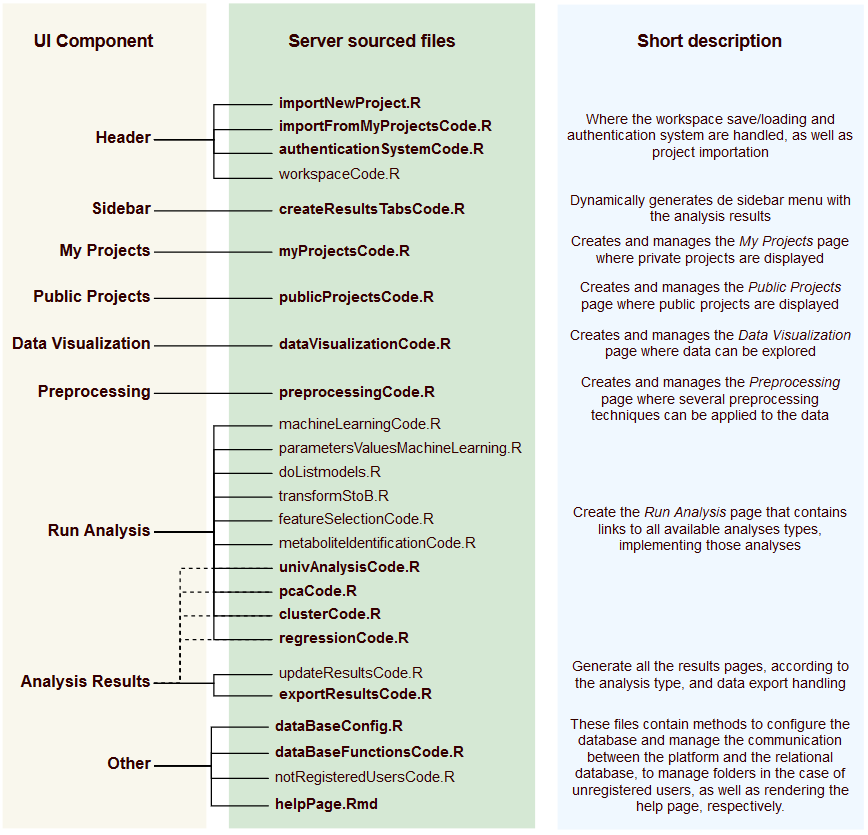
\includegraphics[width=1\linewidth]{Imagens/file_structure}
	\caption{Graphical representation of the application's file structure. The filenames in bold represent the files to which I greatly or totally contributed to, given the scope of this work.}
	\label{file_structure}
\end{figure}

The application layout consists in a dashboard with three components: a header, the sidebar and the body, which was created using the R library \textit{shinydashboard}. 

The dashboard header gives access to the \textit{Data Visualization}, \textit{Pre-processing} and \textit{Run Analysis} modules, as well as the \textit{Saving} and \textit{Loading Workspace} options. The header also includes the option to load a project, which is done through the \textit{Choose Files} button if the user is logged in, or through the \textit{New Project} button if the user is off-line. Lastly, the dashboard header also includes a button to handle the authentication of the user and his account options. 

On the other hand, the dashboard sidebar includes three tabs: the \textit{Home} tab, which represents the main page of the web application; the \textit{My Projects} tab, which contains information about the user's stored projects, and the \textit{Public Projects} tab where all user's shared projects are shown. When a project is loaded the current dataset is also shown on the sidebar. The analysis results can be accessed in the \textit{Analysis Results} menu.

The dashboard organization can be viewed in \autoref{webspecmine_home}.

\begin{figure}[h]
	\centering
	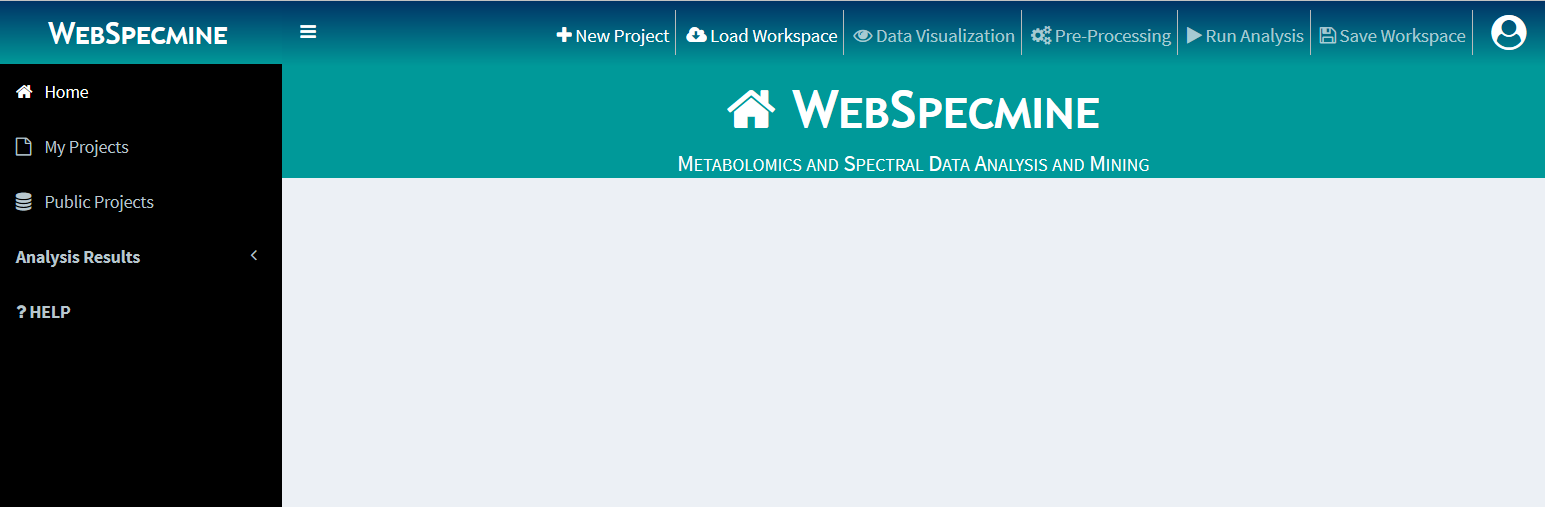
\includegraphics[width=1\linewidth]{Imagens/webspecmine_home}
	\caption{Main page of the web application.}
	\label{webspecmine_home}
\end{figure}

The different modules will be discussed in the following sections.  


\section{Authentication System}

\begin{wrapfigure}{r}{0.40\textwidth}
	\centering
	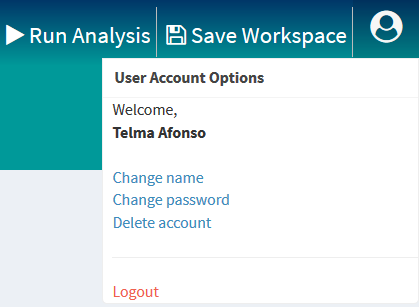
\includegraphics[width=\linewidth]{Imagens/webspecmine_authentication}
	\caption{Authentication menu after successful login (detail).}\label{website_authentication}
\end{wrapfigure}

In the web application, the authentication is made through the \textit{user} button on the upper right corner. Here, the user can either login or register with his e-mail. The password encryption process is explained in \autoref{password}.

Once logged-in, the user has the option to change his name and password, as well as deleting his account, in which case a warning about the account being permanently deleted is shown. The user also has the option to logout, which refreshes the page and the app is set to default values (\autoref{website_authentication}).

%\begin{figure}[h]
%	\centering
%	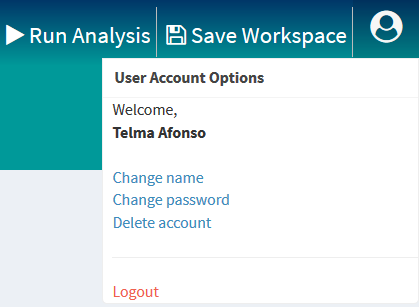
\includegraphics[width=0.6\linewidth]{Imagens/webspecmine_authentication}
%	\caption{Authentication menu after successful login (Zoomed-in).}
%	\label{website_authentication}
%\end{figure}

%\begin{wrapfigure}{r}{2cm}
%	
%	\caption{Authentication menu after successful login (Zoomed-in).}
%	\label{website_authentication}
%	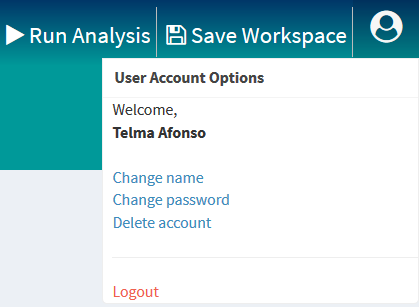
\includegraphics{Imagens/webspecmine_authentication}
%\end{wrapfigure} 



\section{Private and Public Projects}

The modules that handle public and private user's projects are \textit{Public Projects} and \textit{My Projects}, respectively. In this web application, a project is associated with a data folder, which contains sub folders to store one or more datasets that can be of different data types; a metadata folder, which stores one or more metadata files; and a reports folder to store the reports generated during the analysis. A graphical representation of a project's structure is shown in \autoref{project}.

\begin{figure}[h]
	\centering
	\includegraphics[width=0.5\linewidth]{Imagens/project}
	\caption{Graphical representation of a project's structure.}
	\label{project}
\end{figure}

To access the \textit{My Projects} page, the user must be authenticated. Here, all the user's saved projects are displayed, including each project's description, datasets, metadata and report files. 

The user is able to create new projects and data folders for each project and also to edit their information, including the data type in the case of a data folder or name and description in both cases. Both projects and folders can be deleted.

For each data and metadata folder one or multiple files can be uploaded, which can be later used in an analysis. When creating a project the user can decide whether or not to make it public, in which case it will be available for every user. The project status can be changed at anytime using the circular button for the effect. All the user's stored files in this module can be viewed or downloaded at any time. A zoomed view of the \textit{My Projects} page with the metadata tab selected is shown in \autoref{webspecmine_myprojs}.

\begin{figure}[h]
	\centering
	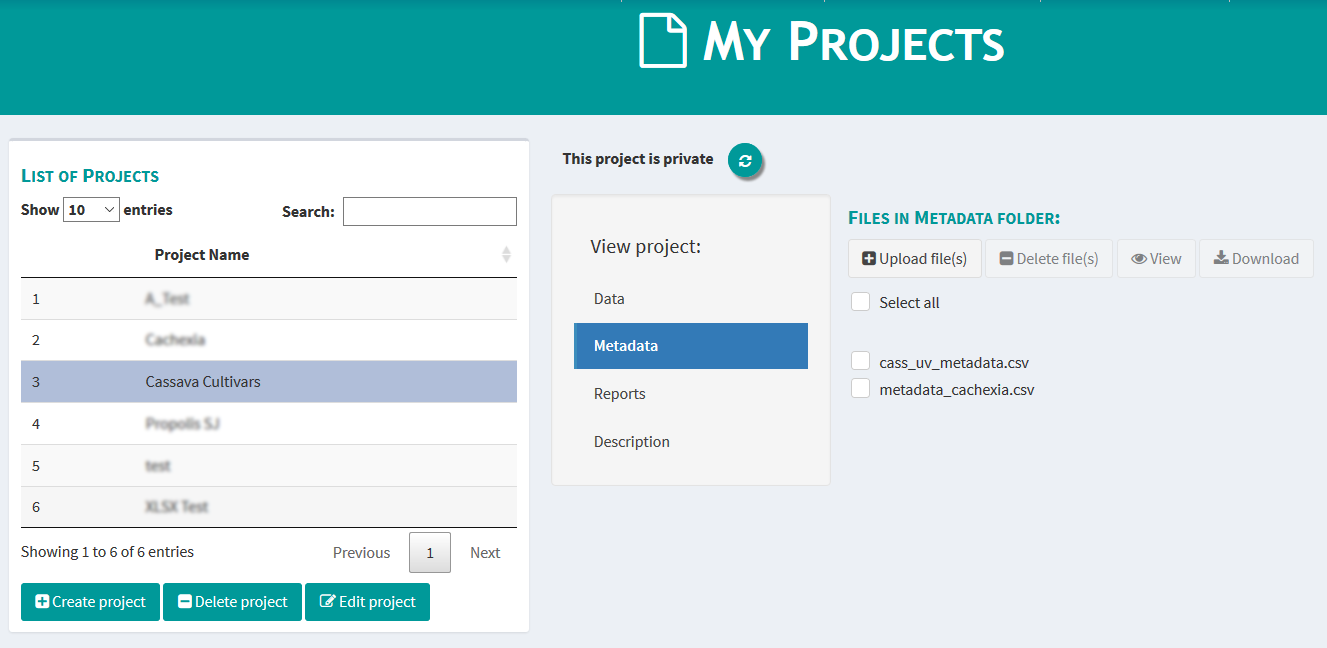
\includegraphics[width=0.9\linewidth]{Imagens/webspecmine_myprojs}
	\caption{Zoomed view over \textit{My Projects} page.}
	\label{webspecmine_myprojs}
\end{figure}

The \textit{Public Projects} module can be accessed without any kind of authentication. Here, all projects that have been made public are displayed in table format, with information about the project name, author and data type. Any project can be imported into the user's private projects collection, given that the project itself is not owned by the user and he does not already own a project by that name. Each project in this module has a description, data, metadata and reports files associated, as in the previous module, that can be viewed at any given time. To obtain the latest list of public projects a \textit{refresh} button is provided.

An important feature also present in the web application is the ability to save and load the workspace. This way, all the data and results the user is currently working on can be saved into his account for later use, thus providing the ability to continue the analysis at any given time.

\section{Import Files} \label{import_files}

Before any analysis can be made, the data must be loaded into the web application. This is done by clicking the \textit{Choose Files} or \textit{New Project} buttons on the dashboard header, which depends on whether or not the user is authenticated, respectively.

In the case of being authenticated, a window with three sections opens. These sections are related with the project, data folder and metadata file to be imported from the user's projects. After choosing the correct files a new window with options to create the dataset appears, according to the data type. 

For spectral data, the data options consist in choosing the file type, that is, whether the selected folder has a single CSV file or multiple CSV, JDX, SPC or XLSX files, the field separator character, whether the samples are represented in columns or rows and if the file has row/column headers. Metadata options consist in choosing the field separator character and whether the file has row/column headers. Additionally, a short description of the data and the \textit{x} and \textit{y} axis labels may be provided. 

On the other hand, if the user is not authenticated the files must be instead uploaded directly into the web application. However, the data and metadata options are the same as in the previous case. The \textit{New Project} window for spectral data is shown in \autoref{webspecmine_import}.

\begin{figure}[h]
	\centering
	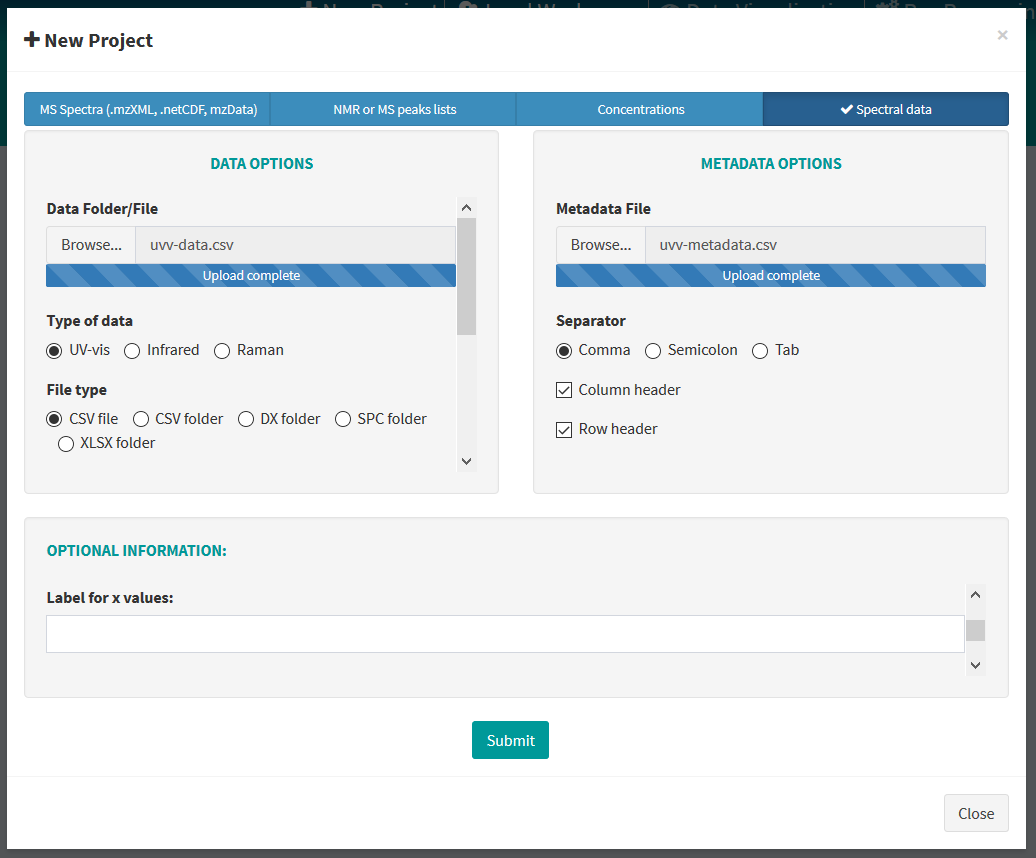
\includegraphics[width=0.8\linewidth]{Imagens/webspecmine_import}
	\caption{Zoomed view over \textit{New Project} window.}
	\label{webspecmine_import}
\end{figure}

In both cases, the \textit{specmine}'s functions used to implement the data reading process are described in \autoref{specmine_functions_data_reading}.


\section{Data Visualization}

When a dataset is loaded, the data and some of its global statistics can be viewed in the \textit{Data Visualization} page. Here, the data and metadata tables, the data summary, a boxplot of the variables and the spectra plot are shown. 

The \textit{Data Summary} tab shows the summary of the loaded dataset, containing the description, type of data, number of samples, data points, metadata variables and missing values, \textit{x} and \textit{y} axis labels, mean, median and range of data values, standard deviation and quantiles of the dataset. The \textit{specmine} function to retrieve the data summary is described in \autoref{specmine_functions_prepocessing}.

In the \textit{Data Table} tab, as the name indicates, a table with all data points is shown, with variables in the rows and samples in the columns. The \textit{Metadata Table}, on the other hand, shows information regarding the metadata, with samples represented in rows and variables in columns. Both tables can be searched for a specific term and ordered by column.

When the loaded dataset is either of the type \gls{nmr}, \gls{ms}, \gls{ir}, \gls{uv} or Raman spectra, an additional tab -- \textit{Spectra Plot} -- is shown, containing the spectra plotted from the dataset, using \textit{specmine}'s \textit{plot\_spectra} function. A number of options are available to adjust the plot, including the metadata variable to color the plot, the samples and the \textit{x} axis range to plot, also including  the option to reverse the \textit{x} axis.  \autoref{data_visualization} shows a zoomed view of the \textit{Spectra Plot} tab in the \textit{Data Visualization} page.

\begin{figure}[h]
	\centering
	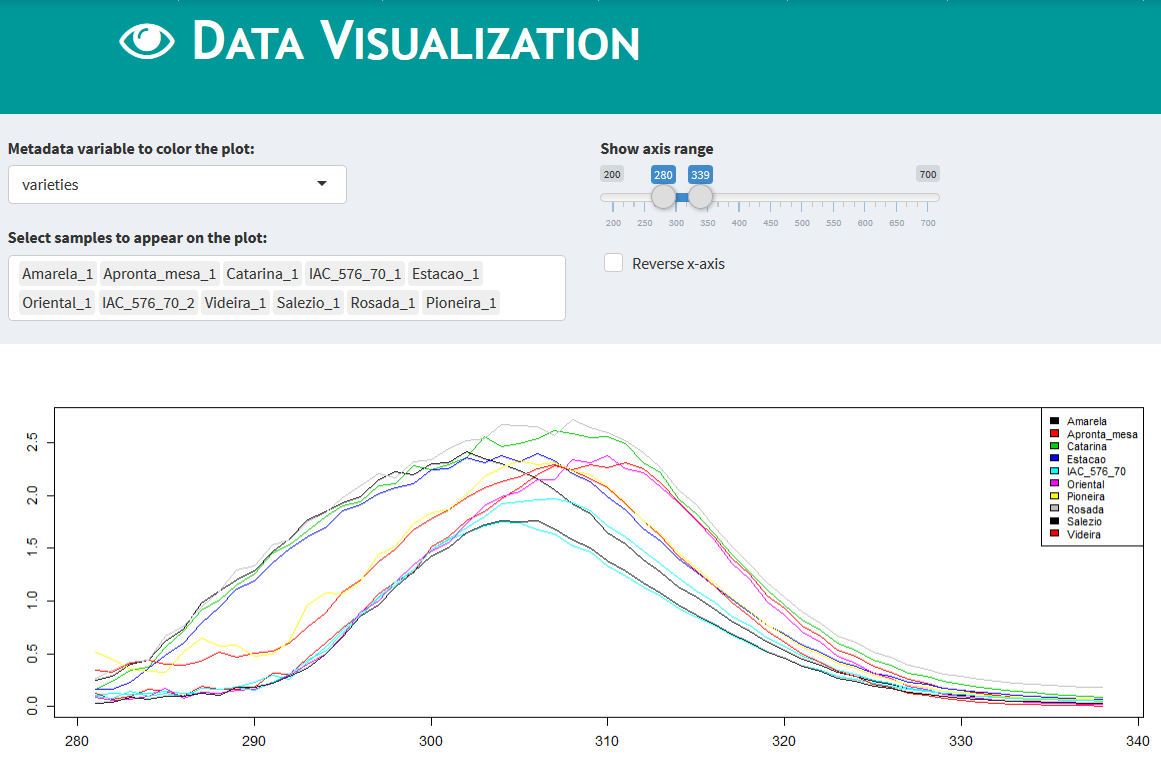
\includegraphics[width=0.9\linewidth]{Imagens/data_visualization}
	\caption{Zoomed view over \textit{Spectra Plot} tab in the \textit{Data Visualization} page.}
	\label{data_visualization}
\end{figure}

Lastly, the \textit{Boxplot of the Variables} tab shows a boxplot that can have from one to the total number of variables plotted, which are selected using a \textit{pickerinput} object from \textit{shinyWidgets} library. The boxplot is plotted using a \textit{specmine} function described in \autoref{specmine_functions_prepocessing}.

An HTML report can be generated with the above information to be either downloaded or saved into the user reports folder of the selected project, in case he is authenticated.



\section{Preprocessing}

On the \textit{Pre-Processing} page, a number of pre-processing approaches can be applied to the data. The page consists in a series of boxes to which a pre-processing technique is assigned to, displayed in two columns format. This way, various techniques can be applied sequentially with a simple mouse click. While some are straightforward to apply, others can be configured with different methods from which to choose from. Some techniques can only be applied to specific types of data or when a condition is met (e.g. missing values can only be treated if the dataset actually has some). After selecting the pre-processing techniques to apply to the data, the user must name the new dataset that is to be created, thus allowing to create multiple versions of the dataset.

A list with all the pre-processing approaches available in the web application and corresponding selectable methods (\textbf{M}), implemented using specmine functions described in \autoref{specmine_functions_prepocessing}, is presented below:


\begin{multicols}{2}
	\begin{itemize}
		\item \textbf{Aggregate samples}
		\item \textbf{Create subset}	
		\item \textbf{Data correction}
		\begin{itemize}
			\item[\textbf{M}] Baseline; background; offset
%			\item[\textbf{F}] \textit{data\_correction}
		\end{itemize}
		\item \textbf{Data normalization}
		\begin{itemize}
			\item[\textbf{M}] Sum; median
%			\item[\textbf{F}] \textit{normalize}
		\end{itemize}
		\item \textbf{Data transformation}
		\begin{itemize}
			\item[\textbf{M}] Logarithmic; cubic root
%			\item[\textbf{F}] \textit{transform\_data}
		\end{itemize}
		\item \textbf{Factor conversion}
%		\begin{itemize}
%			\item[\textbf{F}] \textit{convert\_to\_factor}
%		\end{itemize}
		\item \textbf{First derivative}
%		\begin{itemize}
%			\item[\textbf{F}] \textit{first\_derivative}
%		\end{itemize}
		\item \textbf{Smoothing interpolation}
		\begin{itemize}
			\item[\textbf{M}] Bin; loess; Savitzky-Golay
%			\item[\textbf{F}] \textit{smoothing\_interpolation}
		\end{itemize}
		\item \textbf{Flat patter filter}
		\begin{itemize}
			\item[\textbf{M}] Interquartile range; relative standard deviation; standard deviation; median absolute deviation; mean; median
%			\item[\textbf{F}] \textit{flat\_pattern\_filter}
		\end{itemize}	
		\item \textbf{Mean centering}
%		\begin{itemize}
%			\item[\textbf{F}] \textit{mean\_centering}
%		\end{itemize}
		\item \textbf{Missing value handling}
		\begin{itemize}
			\item[\textbf{M}] Mean; median; given value; \gls{knn}, linear approximation
%			\item[\textbf{F}] \textit{missingvalues\_imputation}
		\end{itemize}
		\item \textbf{\acrlong{msc}}
%		\begin{itemize}
%			\item[\textbf{F}] \textit{msc\_correction}
%		\end{itemize}	
		\item \textbf{Remove data}	
		\item \textbf{Scaling}
		\begin{itemize}
			\item[\textbf{M}] Auto; pareto; range
%			\item[\textbf{F}] \textit{scaling}
		\end{itemize}				
	\end{itemize}
\end{multicols}


%These include mean centering (\textit{mean\_centering}), logarithmic and cubic root data transformations (\textit{transform\_data}), scaling with auto, pareto and range methods (\textit{scaling}), baseline, offset and background corrections (\textit{data\_correction}), smoothing interpolation with methods bin, Loess and Savitzky-Golay (\textit{smoothing\_interpolation}), factor conversion (\textit{convert\_to\_factor}), first derivative (\textit{first\_derivative}), \gls{msc} (\textit{msc\_correction}), data normalization with methods sum and median (\textit{normalize}), missing values handling with methods mean, given value, median, \gls{knn} and linear approximation (\textit{missingvalues\_imputation}), and lastly flat pattern filter with methods interquartile range, relative standard deviation, standard deviation, median absolute deviation, mean and median with option to filter by percentage or threshold (\textit{flat\_pattern\_filter}). 

In \autoref{webspecmine_preprocessing}, a zoomed view of the \textit{Pre-Processing} page is shown, where some of the already mentioned methods, such as missing value handling, mean centering, data transformation, scaling and flat patter filter are emphasized.

\begin{figure}[h]
	\centering
	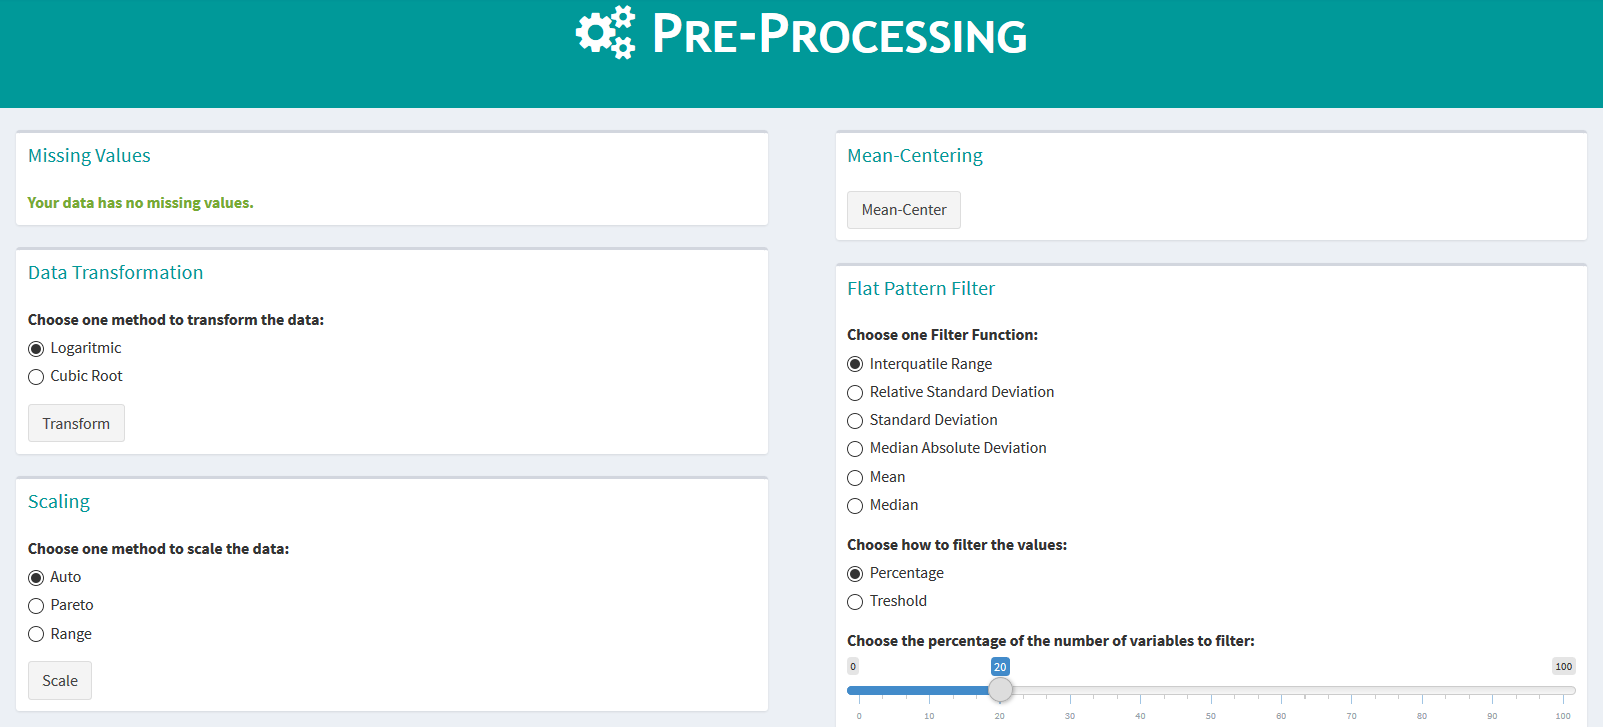
\includegraphics[width=1\linewidth]{Imagens/webspecmine_preprocessing}
	\caption{Zoomed view over \textit{Pre-Processing} page.}
	\label{webspecmine_preprocessing}
\end{figure}



\section{Data Analysis}

Opening the \textit{Run Analysis} page is the first step to perform data analysis using the web application. In this page, each analysis type (or group of analysis) is assigned to a panel with the respective information and a button that leads into the corresponding analyses page, (\autoref{webspecmine_runanalysis}). Currently, there are available univariate analysis such as \gls{anova}, fold change analysis, T-Tests, Kruskal-Wallis and Kolmogorov-Smirnov tests. Unsupervised multivariate analysis include \gls{pca}, hierarchical and k-means clustering and correlation analysis. Other available supervised analyses are machine learning, regression analysis, feature selection and metabolite identification. Since the data types emphasized throughout this work (\gls{uv}, \gls{ir} and Raman) are not usually employed in metabolite identification this type of analysis won't be here discussed. 

\begin{figure}[h]
	\centering
	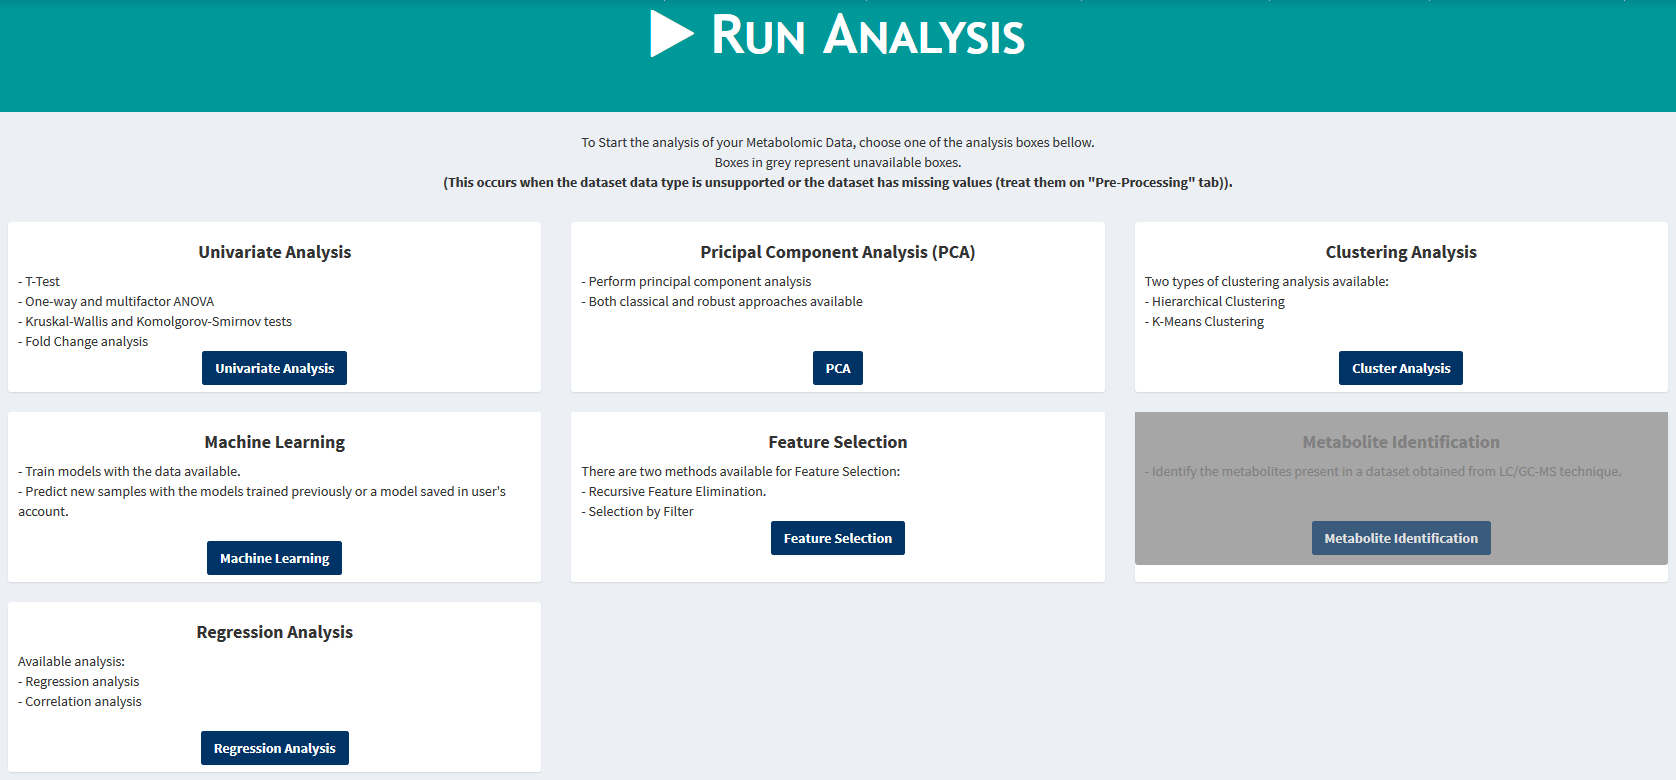
\includegraphics[width=1\linewidth]{Imagens/webspecmine_runanalysis}
	\caption{Zoomed view over the \textit{Run Analysis} page.}
	\label{webspecmine_runanalysis}
\end{figure}

To perform any type of the described methods, a name must be given to the analysis, this being the name that will appear under the corresponding analysis tab in the \textit{Analysis Results} menu on the sidebar. Upon clicking an analysis name, the corresponding results page is opened. Every results page has a round button displayed on the top left corner, which can be clicked to reveal the options used to perform the analysis. It is also important to note that HTML reports and CSV files can be generated with the results at any time, which can then be downloaded and/or saved into the respective project's reports folder. 


\subsection{Univariate Data Analysis}

Regarding univariate data analysis, the web application is able to perform either one-way or multi-factor \gls{anova}, T-Tests, Kruskal-Wallis and Kolmogorov-Smirnov tests, and fold change analysis. These analyses are implemented  using \textit{specmine}'s functions described in \autoref{specmine_functions_analysis}. 

\subsubsection{One-Way Analysis Of Variance}

When performing a one-way \gls{anova} the user must select the metadata variable to use and whether the Tuckey's \gls{hsd} test should be applied. Plot options include the p-value threshold and whether the \textit{x} axis should be reversed. In the results page, a table with the p-value, logarithm of p-value, \gls{fdr} and Tuckey's test results, if it was selected during the analysis, is shown. The table results are ordered by p-value, but can be also ordered by any other result type and searched for a specific term (\autoref{webspecmine_anova}). For this type of analysis, a plot is also shown, with the negative base 10 logarithm of the p-value represented on the \textit{y} axis and variables represented on the \textit{x} axis. 

\begin{figure}[h]
	\centering
	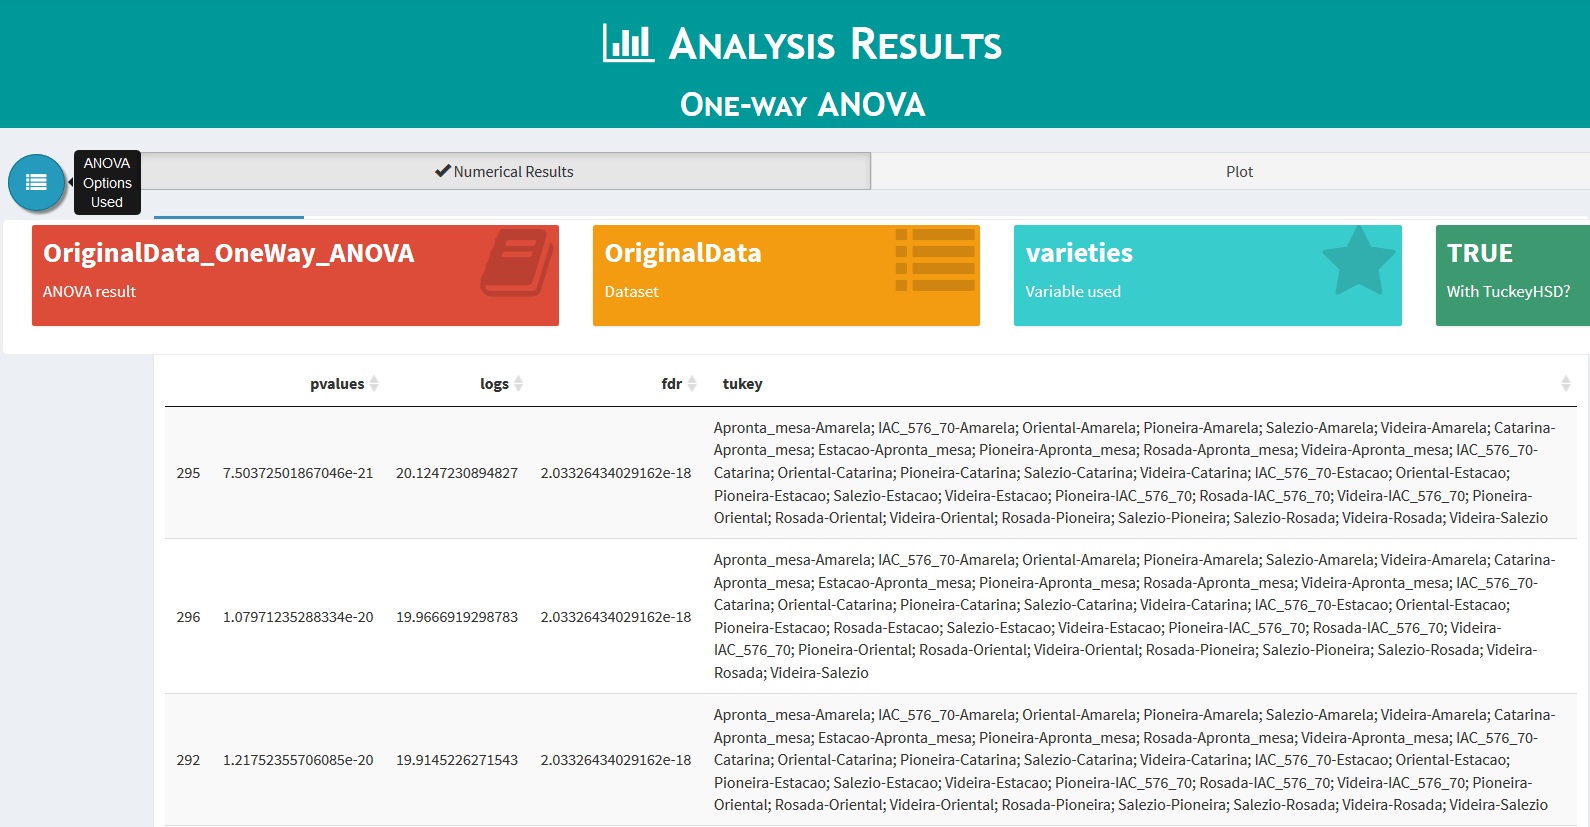
\includegraphics[width=1\linewidth]{Imagens/webspecmine_anova}
	\caption{Zoomed view over \textit{Analysis Results} page for one-way \gls{anova}, showing the numerical results tab and emphasizing the options used for the analysis.}
	\label{webspecmine_anova}
\end{figure}

\subsubsection{Multi-factor Analysis Of Variance}

For the multi-factor \gls{anova}, the metadata variables need to be selected and then a formula, using the selected variables, chosen. The results page for this type of analysis includes a table with the result for each variable on the data, with information regarding the degrees of freedom, sum of squares, mean square, F value, P-value and explained variability.

\subsubsection{T-Tests, Kruskal-Wallis and Kolmogorov-Smirnov Tests}

To run a T-Test, Kruskal-Wallis or Kolmogorov-Smirnov test for each variable from the dataset the user must start by choosing the metadata variable to create the groups of samples as well as the threshold value for the p-value to be considered significant. The results page for the three types of tests are similar, including a table with the p-values, $-log_{\text{10}}$ of the p-values and the \acrlong{fdr}, while also including a plot with variables in the \textit{x} axis and the $-log_{\text{10}}$ of the p-values in the \textit{y} axis.

\subsubsection{Fold Change Analysis}

Two types of fold change analysis can be performed using the web application: either perform the analysis on the entire dataset or over two variables. In the latter case, instead of having the difference of the variables on two groups, the difference of the groups on two variables is calculated. In both cases, the metadata variable to use must be chosen. 

The fold change analysis over the entire dataset requires the user to choose a reference value, namely a class of the metadata variable, while the analysis over two variables requires the user to choose the two variables to use. In the results page, a table with fold change values and the $log_{\text{2}}$ of fold change is shown. It also includes a plot with these $log_{\text{2}}$ of fold change values in the \textit{y} axis and the variable names in the \textit{x} axis, for the analysis over the entire dataset.


\subsection{Linear Regression Analysis}

To perform linear regression analysis, the metadata variables to use must be selected, as well as a formula specifying the model. The results page for this type of analysis includes tables with the p-values, coefficients, r-squared and adjusted r-squared values. It is also possible to plot the linear regression coefficient and the p-values for selected variables, with options to customize the color of the bars and font size.



\subsection{Unsupervised Multivariate Analysis}

Regarding unsupervised multivariate data analysis, the web application is able to perform either classical or robust \gls{pca}, hierarchical and k-means clustering and correlation analysis using \textit{specmine}'s functions described in \autoref{specmine_functions_analysis}.


\subsubsection{Principal Components Analysis}

The simple form of \gls{pca} requires the user to decide if variables are to be scaled and/or centered, while the robust approach allows the centering and scaling methods to be chosen, as well as the number of components. Centering can be done either by mean or median, while scaling methods include standard deviation ratio and mean absolute deviation.

The results pages for both approaches have three tabs: one with the numerical results, another to make the plots and finally a tab where the plots can be visualized. The numerical results tab includes tables with the component importance, the scores matrix and variable loadings for both approaches, while robust \gls{pca} results also include the order of the components.

Available plots are highly customizable, with options that range from selecting the variables to plot to more aesthetic options such as color palette selection (\autoref{webspecmine_pca}A). The available plots in the web application are listed below:

\begin{itemize}
	\item \textbf{Scree plot:} Shows the individual percentages of the explained variance of each principal component and cumulative;
	
	\item \textbf{Pairs plot:} Shows the pairs plot of the scores of the defined principal components, for a chosen variable (\autoref{webspecmine_pca}B);
	
	\item \textbf{Scores plot:} Both 2D and 3D plots that show the scores of two different principal components;
	
	\item \textbf{Biplot:} Plot that displays samples as points, while the variables are displayed either as vectors, linear axes or nonlinear trajectories, considering PC1 and PC2 as axes;
	
	\item \textbf{K-means 2D and pairs plot:} Plots that combine some of the already mentioned plots with k-means results for coloring the points according to the cluster they belong.
			
\end{itemize}


\begin{figure}[h]
	\centering
	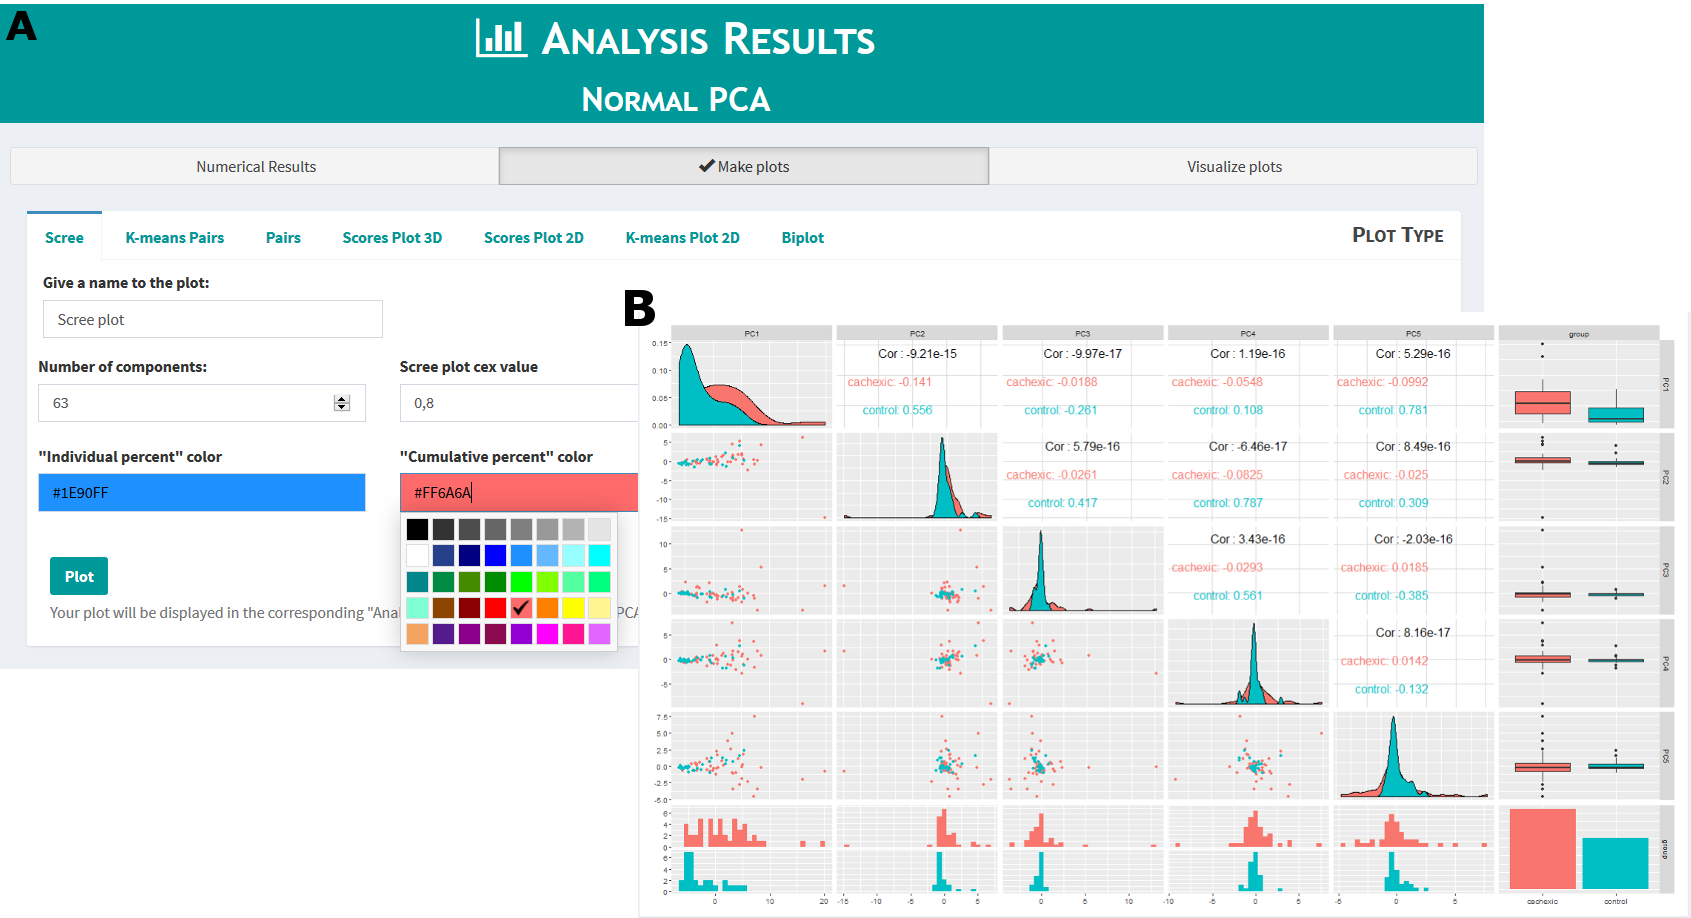
\includegraphics[width=1\linewidth]{Imagens/webspecmine_pca}
	\caption{Zoomed view over the \textit{Analysis Results} page for \gls{pca}, showing the \textit{Make Plots} tab for the scree plot, emphasizing the customizable options (\textbf{A}) and example of a pairs plot made in the web application (\textbf{B}).}
	\label{webspecmine_pca}
\end{figure}


\subsubsection{Clustering Analysis}

Both hierarchical and k-means clustering approaches are available. The former requires the user to select the distance measure (methods include Euclidean, Manhattan, Pearson correlation and Spearman correlation), the agglomeration method (complete, Ward, single, average, McQuitty, median and centroid methods available), and whether to perform the analysis over samples or variables. Additionally, a variable to color the leafs may be chosen. On the other hand, k-means clustering only requires the user to choose the number of clusters and whether to perform the analysis over samples or variables.

The results page for hierarchical clustering analysis includes the resulting dendrogram (\autoref{webspecmine_clustering}), as well as numerical results that comprise heights, order and the labels for the chosen variable to perform the analysis. The dendrogram is plotted using the respective \textit{specmine} function described in \autoref{specmine_functions_analysis}, allowing the dendrogram to show colored leafs, according to the selected variable.

\begin{figure}[h]
	\centering
	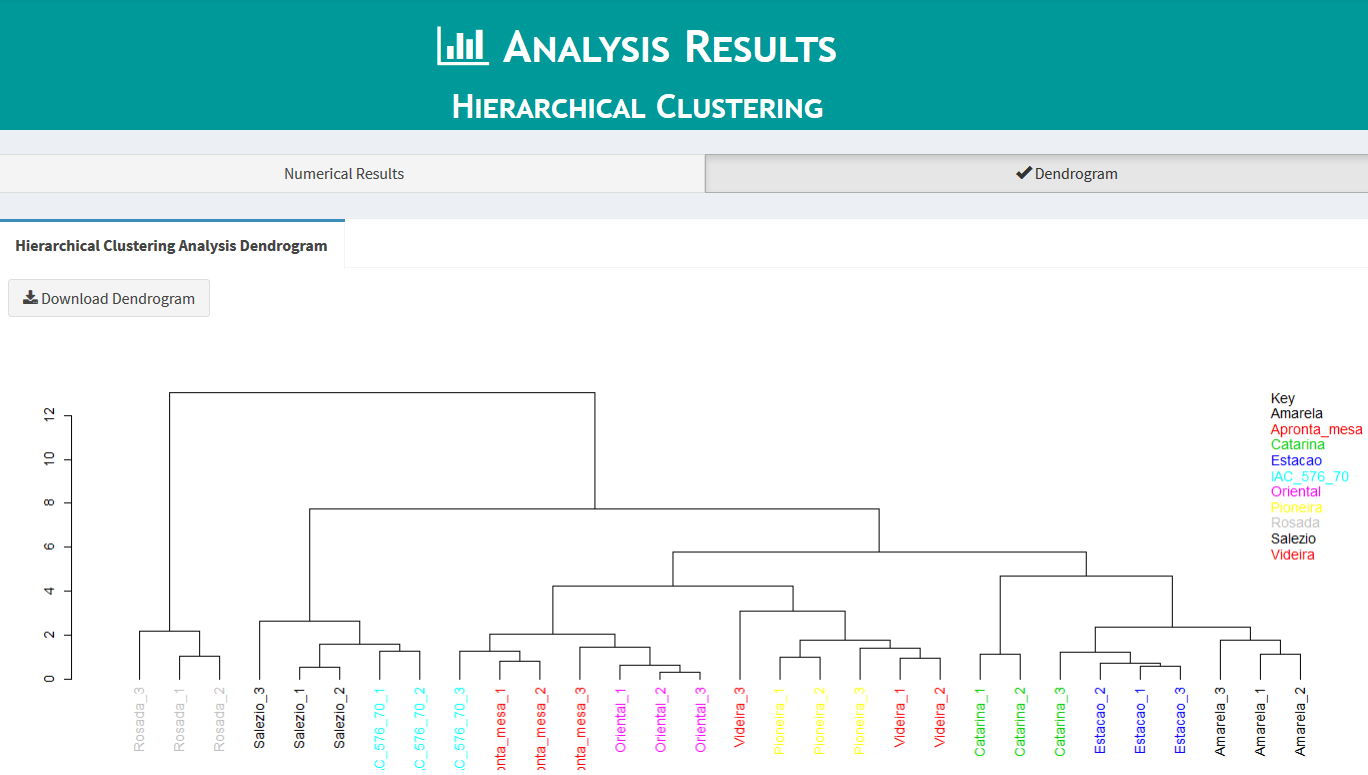
\includegraphics[width=0.9\linewidth]{Imagens/webspecmine_clustering}
	\caption{Zoomed view over \textit{Analysis Results} page for hierarchical clustering, showing the clustering dendrogram.}
	\label{webspecmine_clustering}
\end{figure}

The k-means clustering results page shows information regarding each sample's cluster, the set of samples belonging to each cluster, the centers and the number of samples per cluster. For each cluster a plot is also available, showing in blue the median of the values of the samples in that cluster and in grey all the values of those samples. These plots are implemented using the functions described in \autoref{specmine_functions_analysis}.



\subsubsection{Correlation Analysis}

To perform a correlation analysis between samples or variables the correlation method must be chosen. Three methods are available: Pearson, Kendall and Spearman. The color palette to use in the heatmap is also customizable, with a wide variety of colour gradients available to choose from.

Additionally, a correlations test can be performed over the entire dataset. In such a case, the alternative hypothesis to test must be chosen, and it can be two-sided, greater (for positive association) and less (for negative association).

The results page for this type of analysis includes the correlation matrix and, if a test was performed, the table with the correlation test results. A heatmap is also generated using the correlation matrix, with respective colour scale legend for easier interpretation (\autoref{webspecmine_correlation}).

\begin{figure}[h]
	\centering
	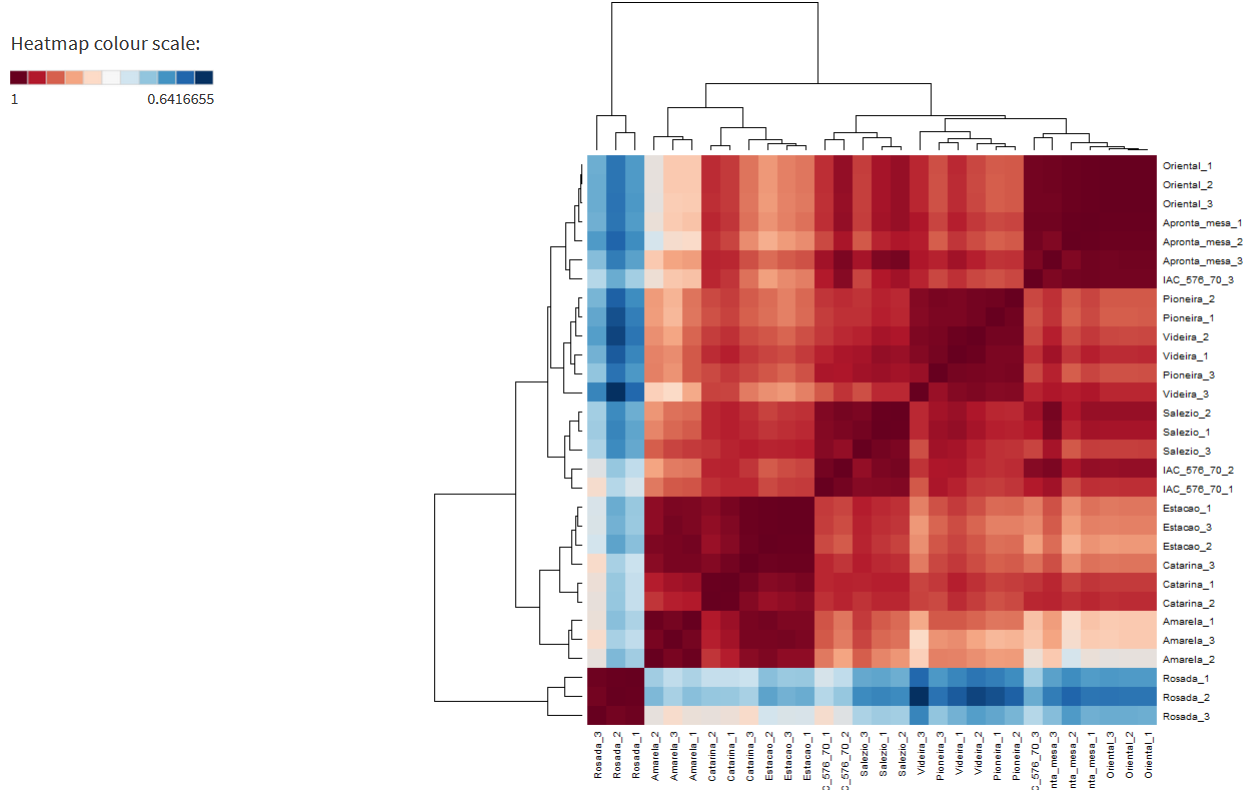
\includegraphics[width=1\linewidth]{Imagens/webspecmine_correlation}
	\caption{Zoomed view over the \textit{Analysis Results} page for correlation analysis, emphasizing the correlation heatmap and respective colour scale.}
	\label{webspecmine_correlation}
\end{figure}



\subsection{Supervised Multivariate Analysis: Machine Learning}

As mentioned before the platform development was shared and this module was not implemented by me, therefore this module will be briefly described.

Regarding machine learning analysis, the web application can perform both model training and prediction of new samples, by implementing \textit{specmine} functions present in \autoref{specmine_functions_machine_learning}. Available models include \gls{pls}, \gls{lda}, decision trees (C4.5-like Trees), rule-based classifier (JRip method), \gls{svm}s with linear kernel, random forests and neural networks. Parameter optimization options are also included. 

%The tunable parameters for the different models are: the number of components for \gls{pls} model, the pruning confidence threshold and minimum instances per leaf for decision tree model, the number of optimizations, folds and weights for rule-based model, the misclassifying influence for \gls{svm} model, the number of variables randomly sampled as candidates at each split for random forests model and the weight decay and number of hidden units for neural network model.

Model validation can be done using resampling, cross-validation, repeated cross-validation, leave-one-out cross-validation and leave group out cross-validation methods. The number of validation folds as well as the metric to test the models performance can also be chosen. These performance test metrics include accuracy and ROC curves.

%The results page for model training shows a table with model performance for every built model, according to the performance metric chosen when performing the analysis. For each trained model, performance metrics such as accuracy, the kappa statistic as well as the standard deviation of the two are shown, alongside the best model parameters and the confusion matrix. The confusion matrix allows to visualize the performance of a model, by showing how many samples were correctly classified or misclassified. The already mentioned performance metrics are also shown for the different number of values tested in each parameter of the models. The overall variable importance as well as its mean are shown in a table for each model, thus completing the results (\autoref{webspecmine_ml}).
%
%\begin{figure}[h]
%	\centering
%	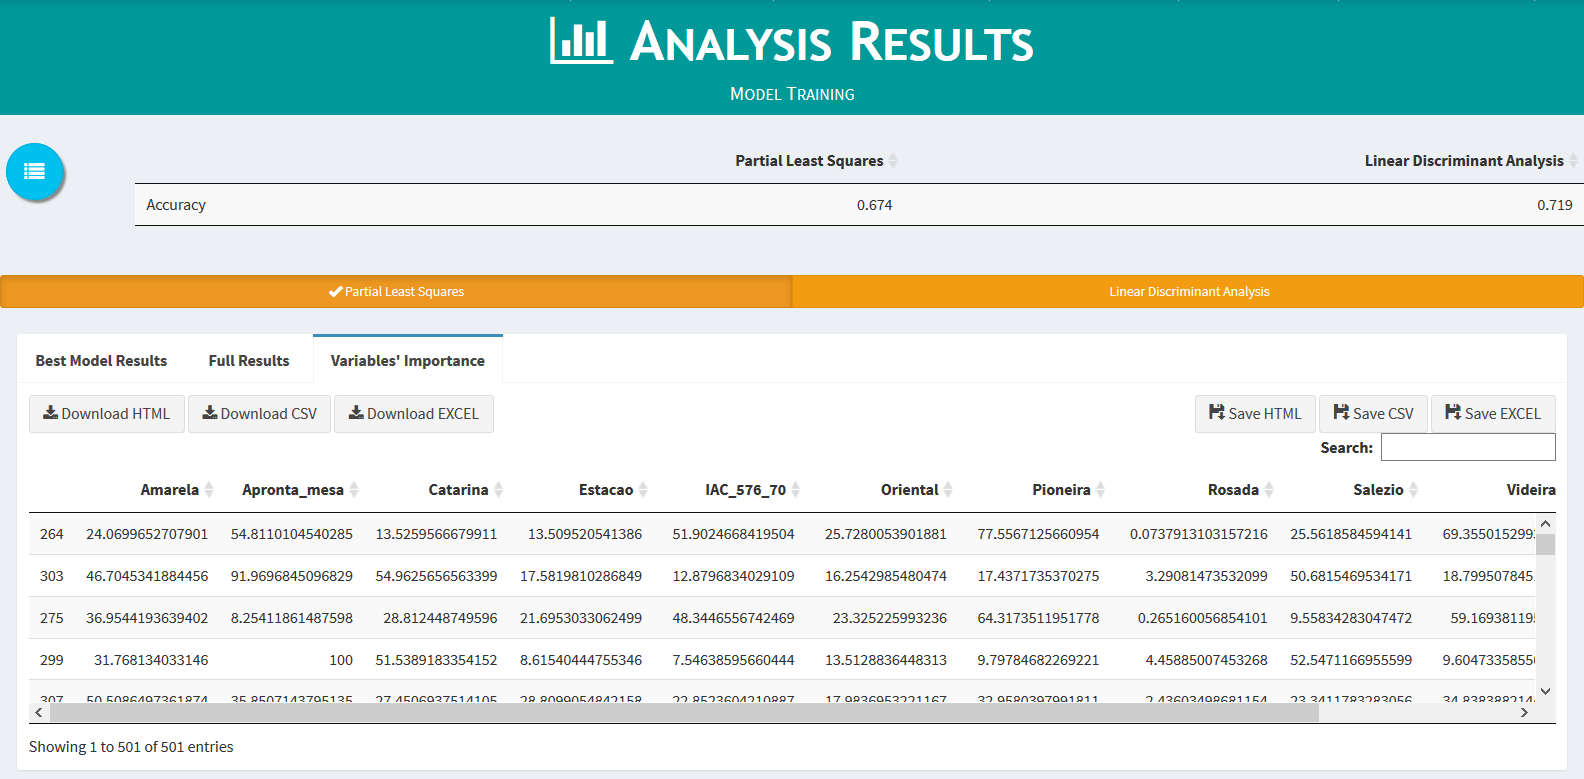
\includegraphics[width=1\linewidth]{Imagens/webspecmine_ml}
%	\caption{Zoomed view over \textit{Analysis Results} page for machine learning \gls{pls} and \gls{lda} model training, emphasizing the results of variable importance.}
%	\label{webspecmine_ml}
%\end{figure}

%To predict new samples, a machine learning model should be previously trained. The user must start by uploading a file containing the dataset with the samples to be predicted, which must be the same dataset used to train the models. The file upload window options are dependent of the data type and are similar to what has been already described in \autoref{import_files}. Upon uploading the file, the samples are further pre-processed similarly to dataset used for model training. Finally one of the trained models is selected and samples can then be predicted.

%Metrics for regression: Root Mean Square Error (RMSE) and the coefficient of determination (R2). Only classification problems?


\subsection{Feature Selection}

Similarly to the previous section, the feature selection module was not developed by me and, therefore, it will be briefly described.

Available feature selection methods include wrappers (\gls{rfe}) and filters. Additionally, the metadata variable where the class to predict is must be chosen, as well as the function for model fitting, prediction and variable importance/filtering, which can be done using random forests, linear regression, bagged trees, \gls{lda} or the Naive-Bayes method. This type of analysis is implemented using \textit{specmine}'s function described in \autoref{specmine_functions_machine_learning}.

%Methods for model validation include bootstrap, cross-validation, repeated cross-validation, leave one out cross-validation and leave group out cross-validation methods. The number of validation folds (or resampling iterations in the case of bootstrap)  and the number of features for each group of test is also selectable.

%The results page for feature selection includes the resampling performance with the already mentioned metrics (accuracy, kappa statistic and their standard deviations), the name of the variables that compose the best subset and the percentage of the variables selected during the resampling. Additionally, a plot with the performance profile across the different subset sizes is also shown.








	
\section{Data Model for Project, Dataset and User Management}

The data model used for the management of the different files and the authentication system will be explained in this and the following section, respectively.

A relational database for project, dataset and user management was created using the MySQL \gls{rdbms}. The tables that constitute the database are the \textit{user}, \textit{project}, \textit{permission}, \textit{dataset} and \textit{datatype} tables. The MySQL model used in the platform for project, dataset and user management is shown in \autoref{database}.

\begin{figure}[h]
	\centering
	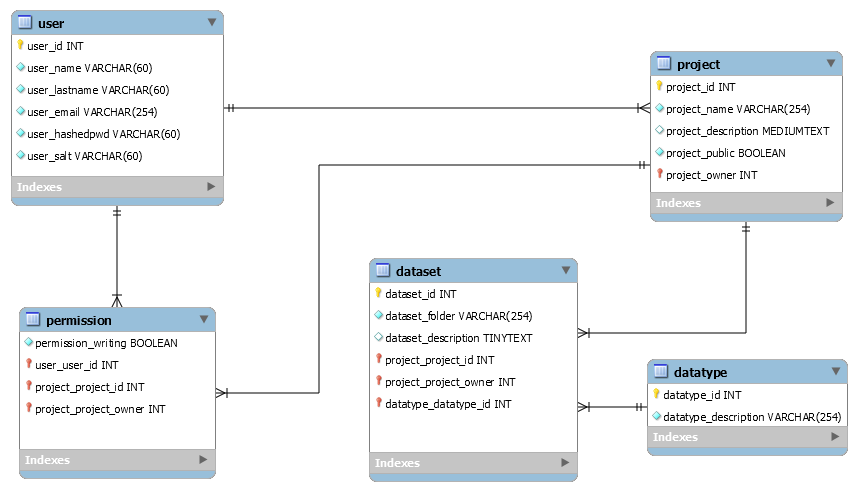
\includegraphics[width=0.95\linewidth]{Imagens/database}
	\caption{MySQL model used in the platform for project, dataset and user management.}
	\label{database}
\end{figure}

The \textit{user} table has a \textit{user\_id} attribute to store each user's unique identifier, a \textit{user\_name} attribute to store the user's first name, a \textit{user\_lastname} attribute to store the user's last name, a \textit{user\_email} attribute to store the user's email, a \textit{user\_hashedpwd} attribute to store the encrypted password and a \textit{user\_salt} attribute which stores the salt associated with the password. The password encryption process will be explained in the next section. 

The \textit{user} table has a 1:N relationship with the \textit{project} table, meaning a user can have one or more projects. \textit{Project} table has a \textit{project\_id} attribute to store each project's identifier, a \textit{project\_name} attribute to store the project's name, a \textit{project\_description} optional attribute to store the project's description, a \textit{project\_public} attribute that stores a boolean value indicating whether or not the project is public and a foreign key \textit{project\_owner} which references to the \textit{user}'s table \textit{user\_id} attribute.

Projects can either be public, and every user has access to them, or private, in which case only the creator has access. These permissions are handled in the \textit{permission} table, which has a \textit{permission\_writing} attribute that stores a Boolean value according to the privacy of a project. Both \textit{user} and \textit{project} tables have a 1:N relationship with the \textit{permission} table. The \textit{user\_user\_id} foreign key references to the \textit{user\_id} attribute in the \textit{user} table, whereas the \textit{project\_project\_id} and \textit{project\_project\_owner} reference to the \textit{project\_id} and \textit{project\_owner} attributes in the \textit{project} table, respectively.

The dataset information is stored in the \textit{dataset} table, which has a \textit{dataset\_id} attribute to store each dataset's unique ID, a \textit{dataset\_folder} attribute to store the dataset name and a \textit{dataset\_description} optional attribute to store the dataset description. Each dataset has an associated data type, which is stored in the \textit{datatype} table. This table has a \textit{datatype\_id} attribute that stores each data type unique ID and a \textit{datatype\_description} attribute to store the data type name. 

Both \textit{datatype} and \textit{project} tables have a 1:N relationship with the \textit{dataset} table. In this table, the \textit{datatype\_datatype\_id} foreign key references to the \textit{datatype\_id} attribute in the \textit{datatype} table, whereas the \textit{project\_project\_id} and \textit{project\_project\_owner} reference to the \textit{project\_id} and \textit{project\_owner} attributes in the \textit{project} table, respectively.

While the management itself is done using the database, the files are stored in the local file system rather than the database, which only stores the paths to the files.


\section{Password Encryption for Authentication System} \label{password}

For the password encryption process the \textit{bcrypt} R package was used (\href{https://CRAN.R-project.org/package=bcrypt}{\nolinkurl{https://CRAN.R-project.org/package=bcrypt}}). It consists in an R  interface to the OpenBSD 'blowfish' password hashing algorithm, as described in \cite{provos1999future}.

Hashing is the transformation of a string of characters into a usually shorter fixed-length value or key that represents the original string. The hashing process is performed by a hash function, whose returned values are often called hash values, hash codes, digests, or simply hashes. This is a one-way function in which a hashed value cannot be reversed to obtain the original input value (i.e. the password). These functions generate random bytes or numbers from OpenSSL (\href{https://www.openssl.org/}{\nolinkurl{https://www.openssl.org/}}). This provides a cryptographically secure alternative to R's default random number generator. 

\textit{Bcrypt} has the option to incorporate a salt, that is, a random data that is used as an additional input to the hash function, providing additional defense against dictionary attacks or against its hashed equivalent, a pre-computed rainbow table attack. \textit{Bcrypt} is an adaptive function: over time, the iteration count can be increased to make it slower, so it remains resistant to brute-force search attacks even with increasing computation power.

For each password chosen by the users a random salt is generated, using the \textit{gensalt} function, which is stored in the database. The password string is then hashed with the generated salt using the \textit{hashph} function, and the hash code stored in the database as well. 

To authenticate a user, when the application receives a username and password, it performs the hashing operation using the password and stored salt and compares the resulting hashed value with the password hash stored in the database for the particular user. If the two hashes are an exact match, the user provided a valid username and password (\autoref{hash}).

\begin{figure}[h]
	\centering
	\includegraphics[width=0.85\linewidth]{Imagens/hash}
	\caption{Graphical representation of the hashing process.}
	\label{hash}
\end{figure}


Below is a simple example of password hashing in R using the \textit{bcrypt} package:


\begin{lstlisting}[language = R]
library(bcrypt)

password = '12345'
salt = gensalt(log_rounds = 12)
salt
## "$2a$12$.RGbTpgZ8TyBpP.MJUFXMu"

hash = hashpw(password, salt)
hash
## "$2a$12$.RGbTpgZ8TyBpP.MJUFXMubcbSTfHve1cnkHohULAIoDLWq580pNG"

identical(hash, hashpw(password, salt))
## TRUE

\end{lstlisting}

The prefix "\$2a\$12\$" in the hash string specifies a cost parameter of 12, indicating $2^{12}$ key expansion rounds. The random generated salt is ".RGbTpgZ8TyBpP.MJUFXMu" and the resulting hash for the "12345" password is ".RGbTpgZ8TyBpP.MJUFXMubcbSTfHve1cnkHoh-ULAIoDLWq580pNG". These are the values that would be stored in the database, rather than the password itself.


	
	
	% CHAPTER - Use Cases
	
	
\chapter{Use Cases} \label{use_cases}

The main purpose of the current chapter is to demonstrate the functionalities of the web platform, by building reproducible analysis pipelines using real data from previously published studies in the host group, while trying to show how to perform most of the available analyses in the web platform. For this purpose, two distinct datasets were used. The first use case is the discrimination of propolis samples from southern Brazil according to their chemical profile (using \gls{uv} data) \citep{tomazzoli2015discrimination}, while the second use case consists in the chemical and enzymatic composition screening in several genotypes of cassava roots during \gls{ppd} (using \gls{ir} data) \citep{uarrota2014metabolomics}.


\section{Propolis}

\subsection{Context}

The propolis resinous substance is collected by honeybees \textit{Apis mellifera} from various plant sources and added to salivary enzymes, beeswax, and pollen. They use it to seal openings and for protection against microorganisms and insects.

However, this substance also offers a broad spectrum of biological activities, including, for instance, cytotoxic, anti-herpes, free radical scavenging, antimicrobial, and anti-HIV activities, being used in both cosmetic and pharmaceutical markets. Therefore, the botanical origin of propolis is extremely important to guarantee that raw materials of superior quality are supplied to those markets.

Since the quality of the propolis depends, among other variables, on the local flora,
which is strongly influenced by (a)biotic factors over the seasons, the main scope of the study was to determine the harvest season effect on the chemical profile of this substance.

For this purpose, propolis samples from \textit{A. mellifera} were collected in Southern Brazil throughout 2014, and samples visually classified according to their color. The \gls{uv} absorbance values were recorded using a spectral window of 280-800 $\eta m$ \citep{tomazzoli2015discrimination}.


\subsection{Data Loading} \label{propolis_loading}

Assuming the user has already created a project with both data and metadata files, the dataset can be easily created through the \textit{Choose Files} button on the header. This step is done by directly importing a project from the user's stored projects and setting the file specifications to create the dataset, as observed in \autoref{propolis_import_project}.

\begin{figure}[h]
	\centering
	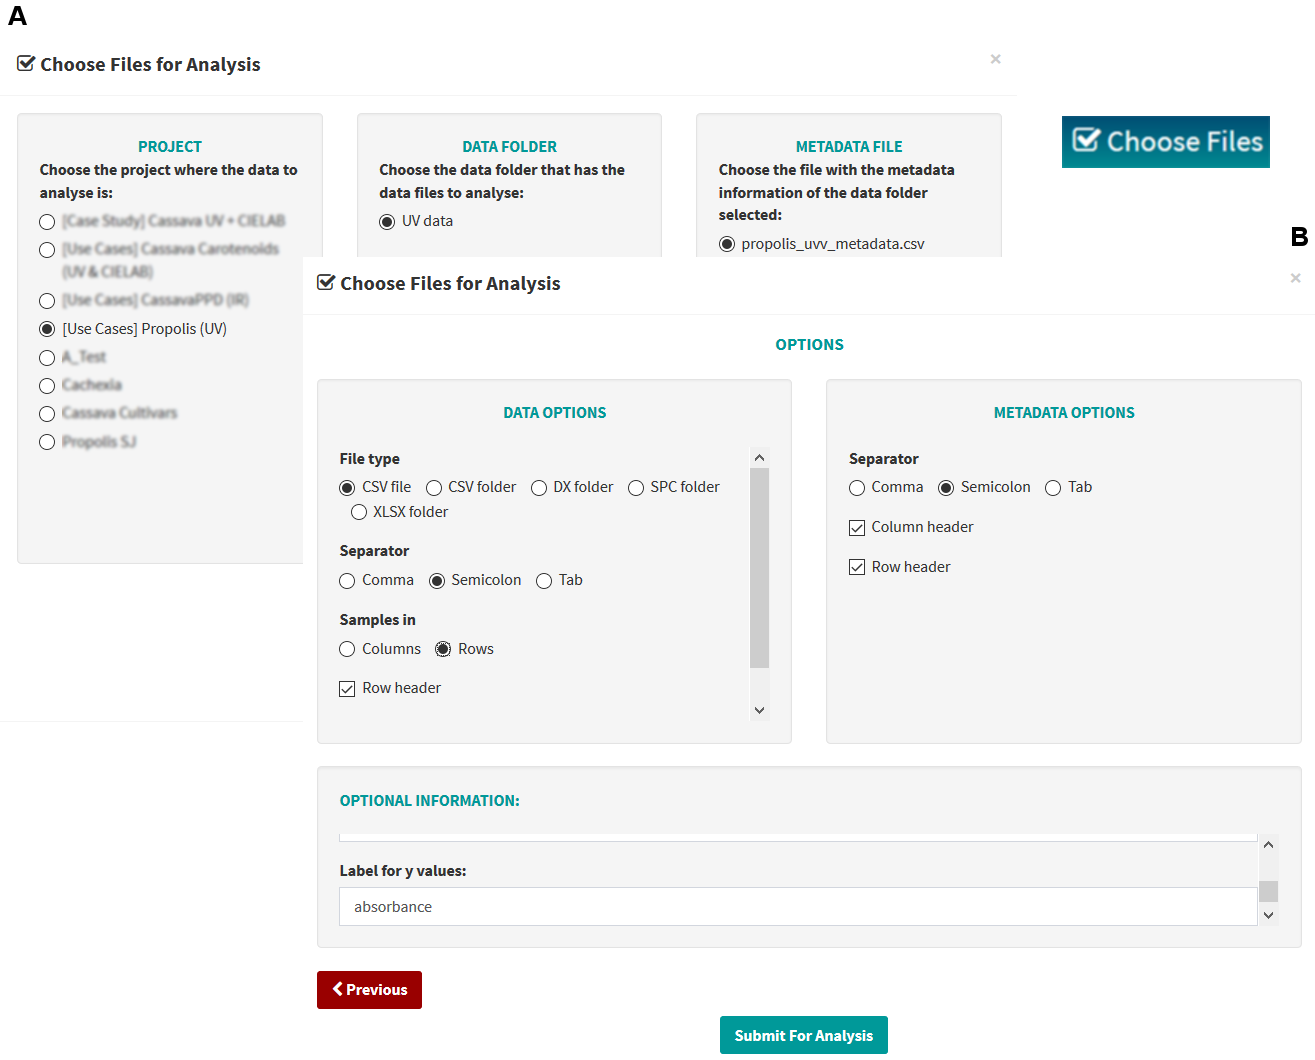
\includegraphics[width=1\linewidth]{Imagens/Propolis/import_project}
	\caption{Creating the propolis dataset for analysis. Upon clicking the \textit{Choose Files} button on the header, a window appears with all user's projects and respective folders/files (\textbf{A}). After selecting the desired project, the file specifications must be chosen to create the dataset (\textbf{B}).}
	\label{propolis_import_project}
\end{figure}


\subsection{Data Overview}

Once the dataset is created, its information can be easily accessed in the \textit{Data Visualization} page. 
In \autoref{propolis_data_overview}, the summary of the propolis dataset, along with the spectra plot colored by the \textit{seasons} metadata variable, and the metadata table are shown. The \gls{uv} dataset has 5 metadata variables, a total of 165 samples and 521 data points, with no missing values.


\begin{figure}[h]
	\centering
	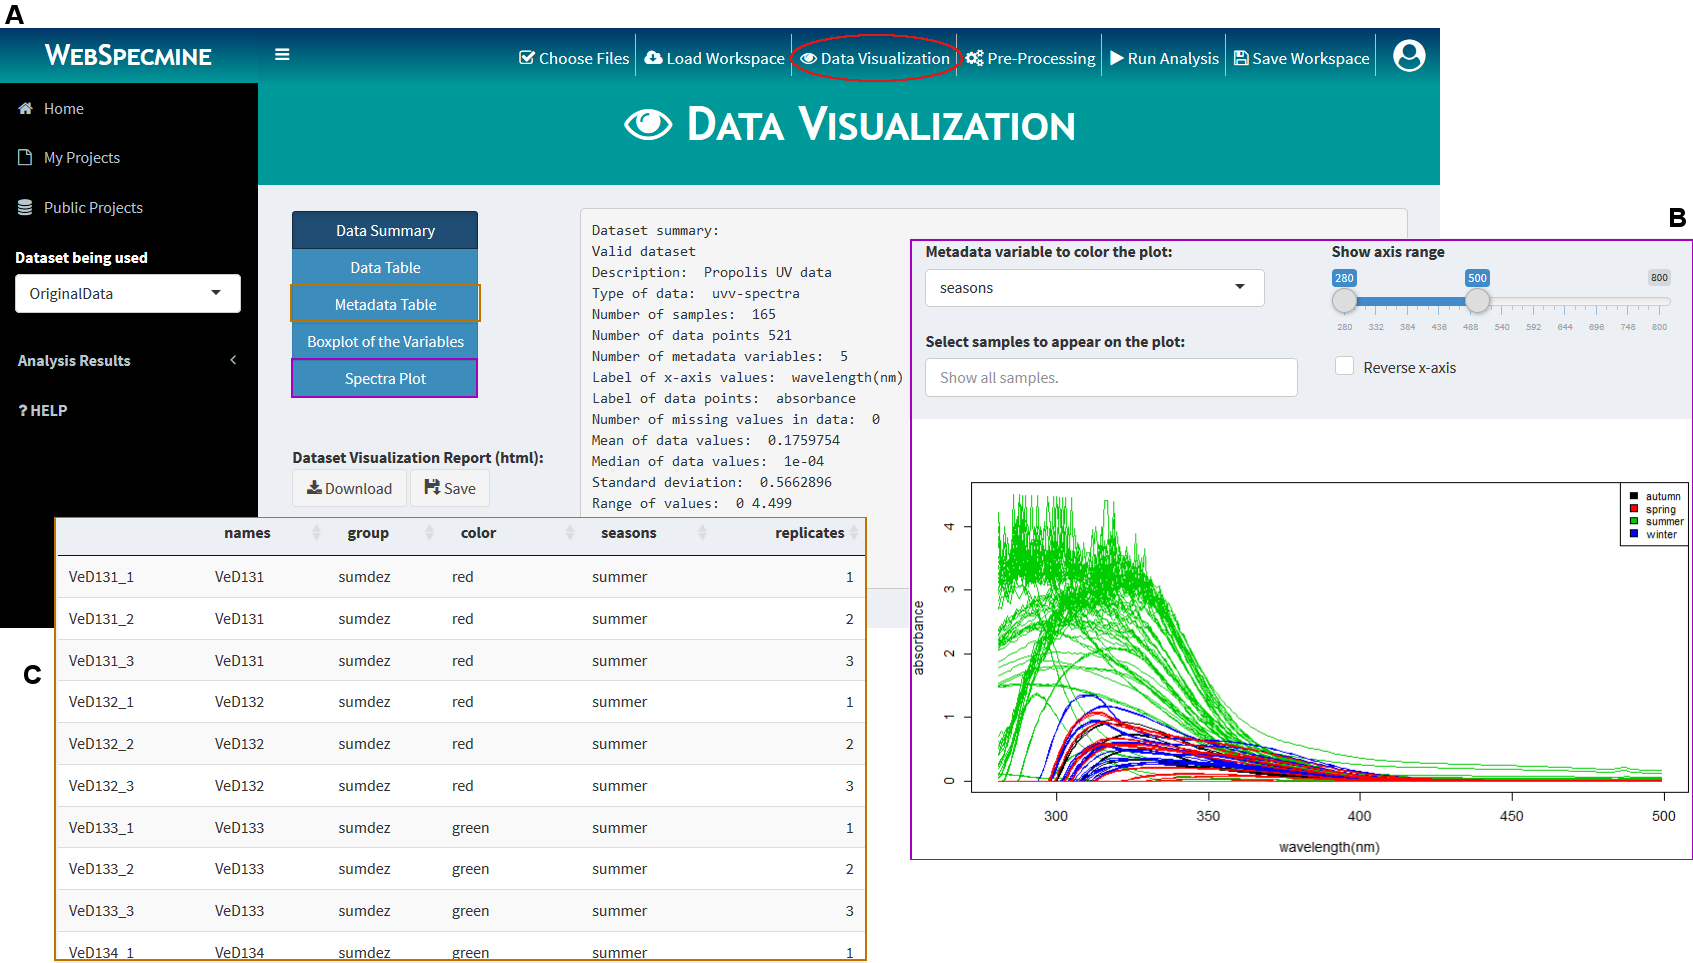
\includegraphics[width=1\linewidth]{Imagens/Propolis/data_overview}
	\caption{The \textit{Data Visualization} page showing the dataset summary (\textbf{A}), the spectra plot colored by the \textit{seasons} metadata variable (\textbf{B}), and the metadata table (\textbf{C}).}
	\label{propolis_data_overview}
\end{figure}


\subsection{Pre-processing}


To apply pre-processing methods to the dataset we go over to the \textit{Pre-Processing} page. Here, four pre-processing methods will be applied, including smoothing interpolation followed by background, offset and baseline corrections. To apply these methods, we simply have to go to the respective method box and, after selecting the parameters accordingly, click the button on the box to apply the selected method. Finally, a name must be given to the new pre-processed dataset and the process is done (\autoref{propolis_proprocessing}).

\begin{figure}[h]
	\centering
	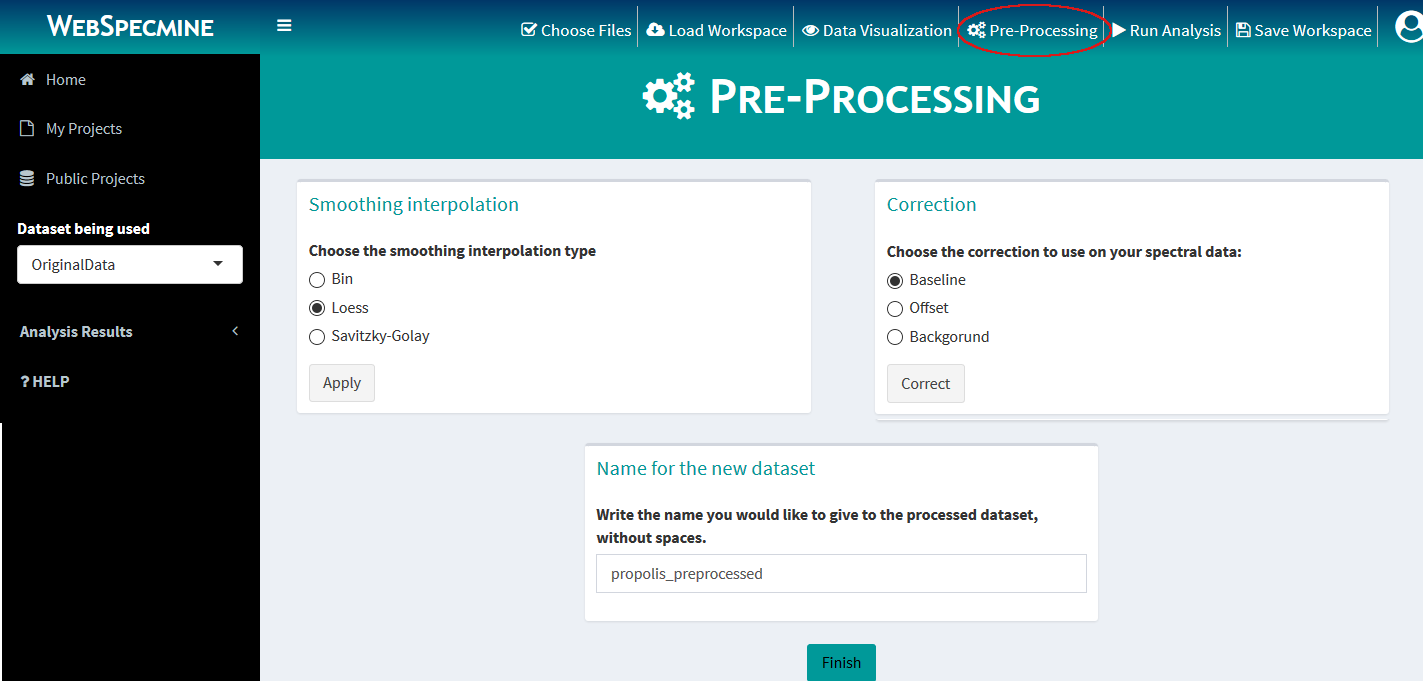
\includegraphics[width=0.8\linewidth]{Imagens/Propolis/proprocessing}
	\caption{The \textit{Pre-Processing} page emphasizing the boxes for smoothing interpolation, background, offset and baseline corrections. Please note the image was edited to emphasize the pre-processing methods used in this example.}
	\label{propolis_proprocessing}
\end{figure}


Returning back to the \textit{Data Visualization} page, the effects of the applied pre-processing methods are noticeable (\autoref{propolis_data_overview_preproc}).


\begin{figure}[H]
	\centering
	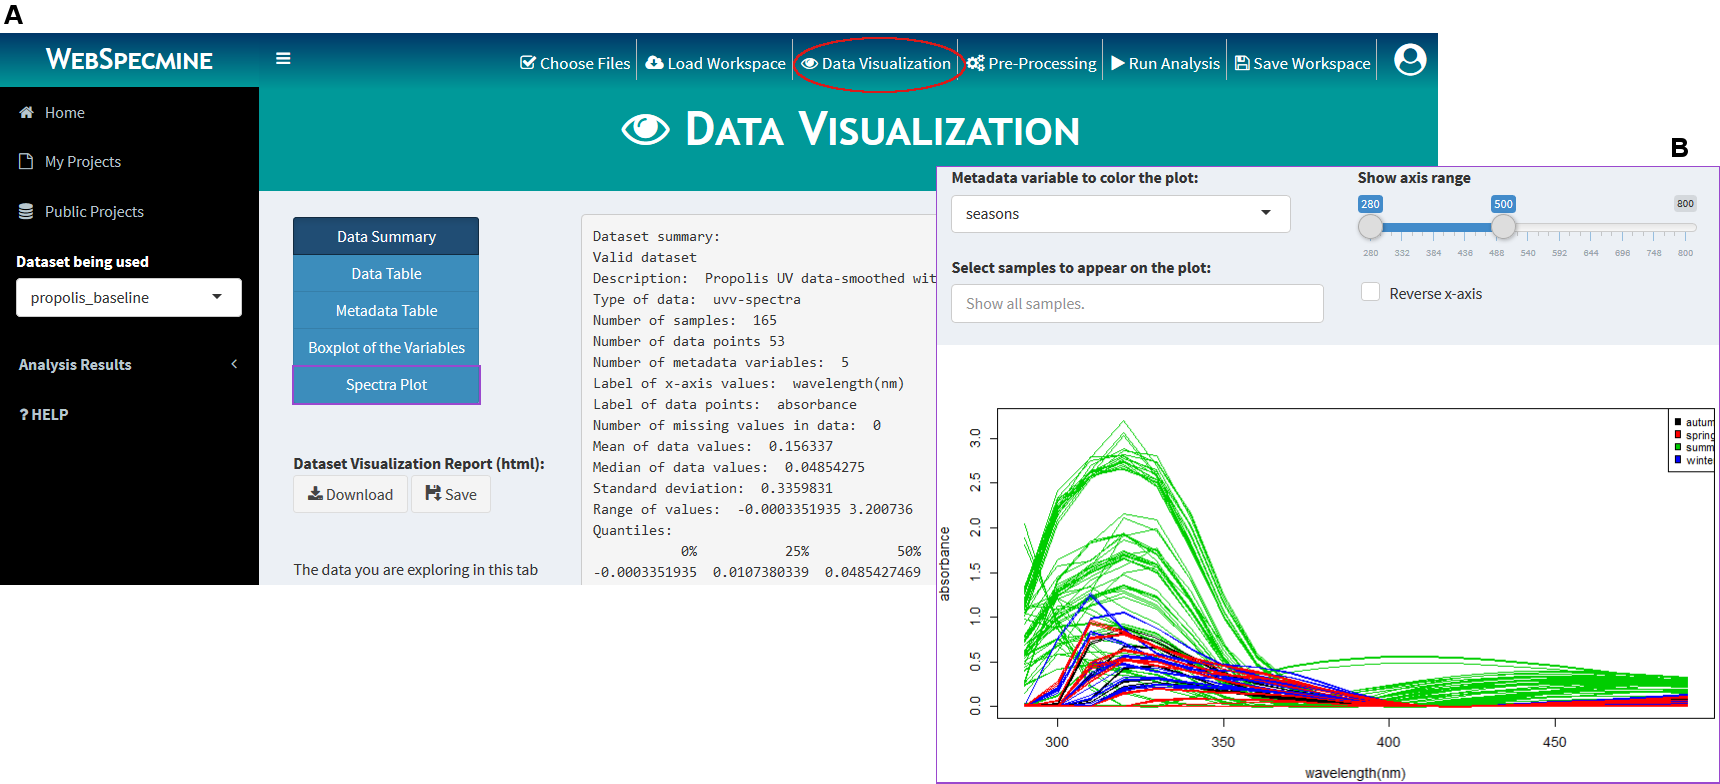
\includegraphics[width=1\linewidth]{Imagens/Propolis/data_overview_preproc}
	\caption{The \textit{Data Visualization} page showing the dataset summary (\textbf{A}) and the spectra plot colored by the \textit{seasons} metadata variable (\textbf{B}) after data pre-processing.}
	\label{propolis_data_overview_preproc}
\end{figure}



\subsection{Univariate Analysis}

The next step is to perform univariate statistical analysis, in this case one-way \gls{anova} given that the \textit{seasons} metadata variable has more than two possible values.
To perform an \gls{anova}, we must go to the \textit{Run Analysis} page and from here select the \textit{Univariate Analysis} box, leading into the analysis page (\autoref{propolis_anova}A). After selecting the analysis options and clicking \textit{Submit}, the analysis is performed and a new page appears with the analysis results (\autoref{propolis_anova}B). This analysis can be accessed anytime by clicking the respective name in the \textit{Analysis Results} menu on the sidebar. In this case, a One-way \gls{anova} with a post-hoc Tukey's \gls{hsd} was performed.

\begin{figure}[H]
	\centering
	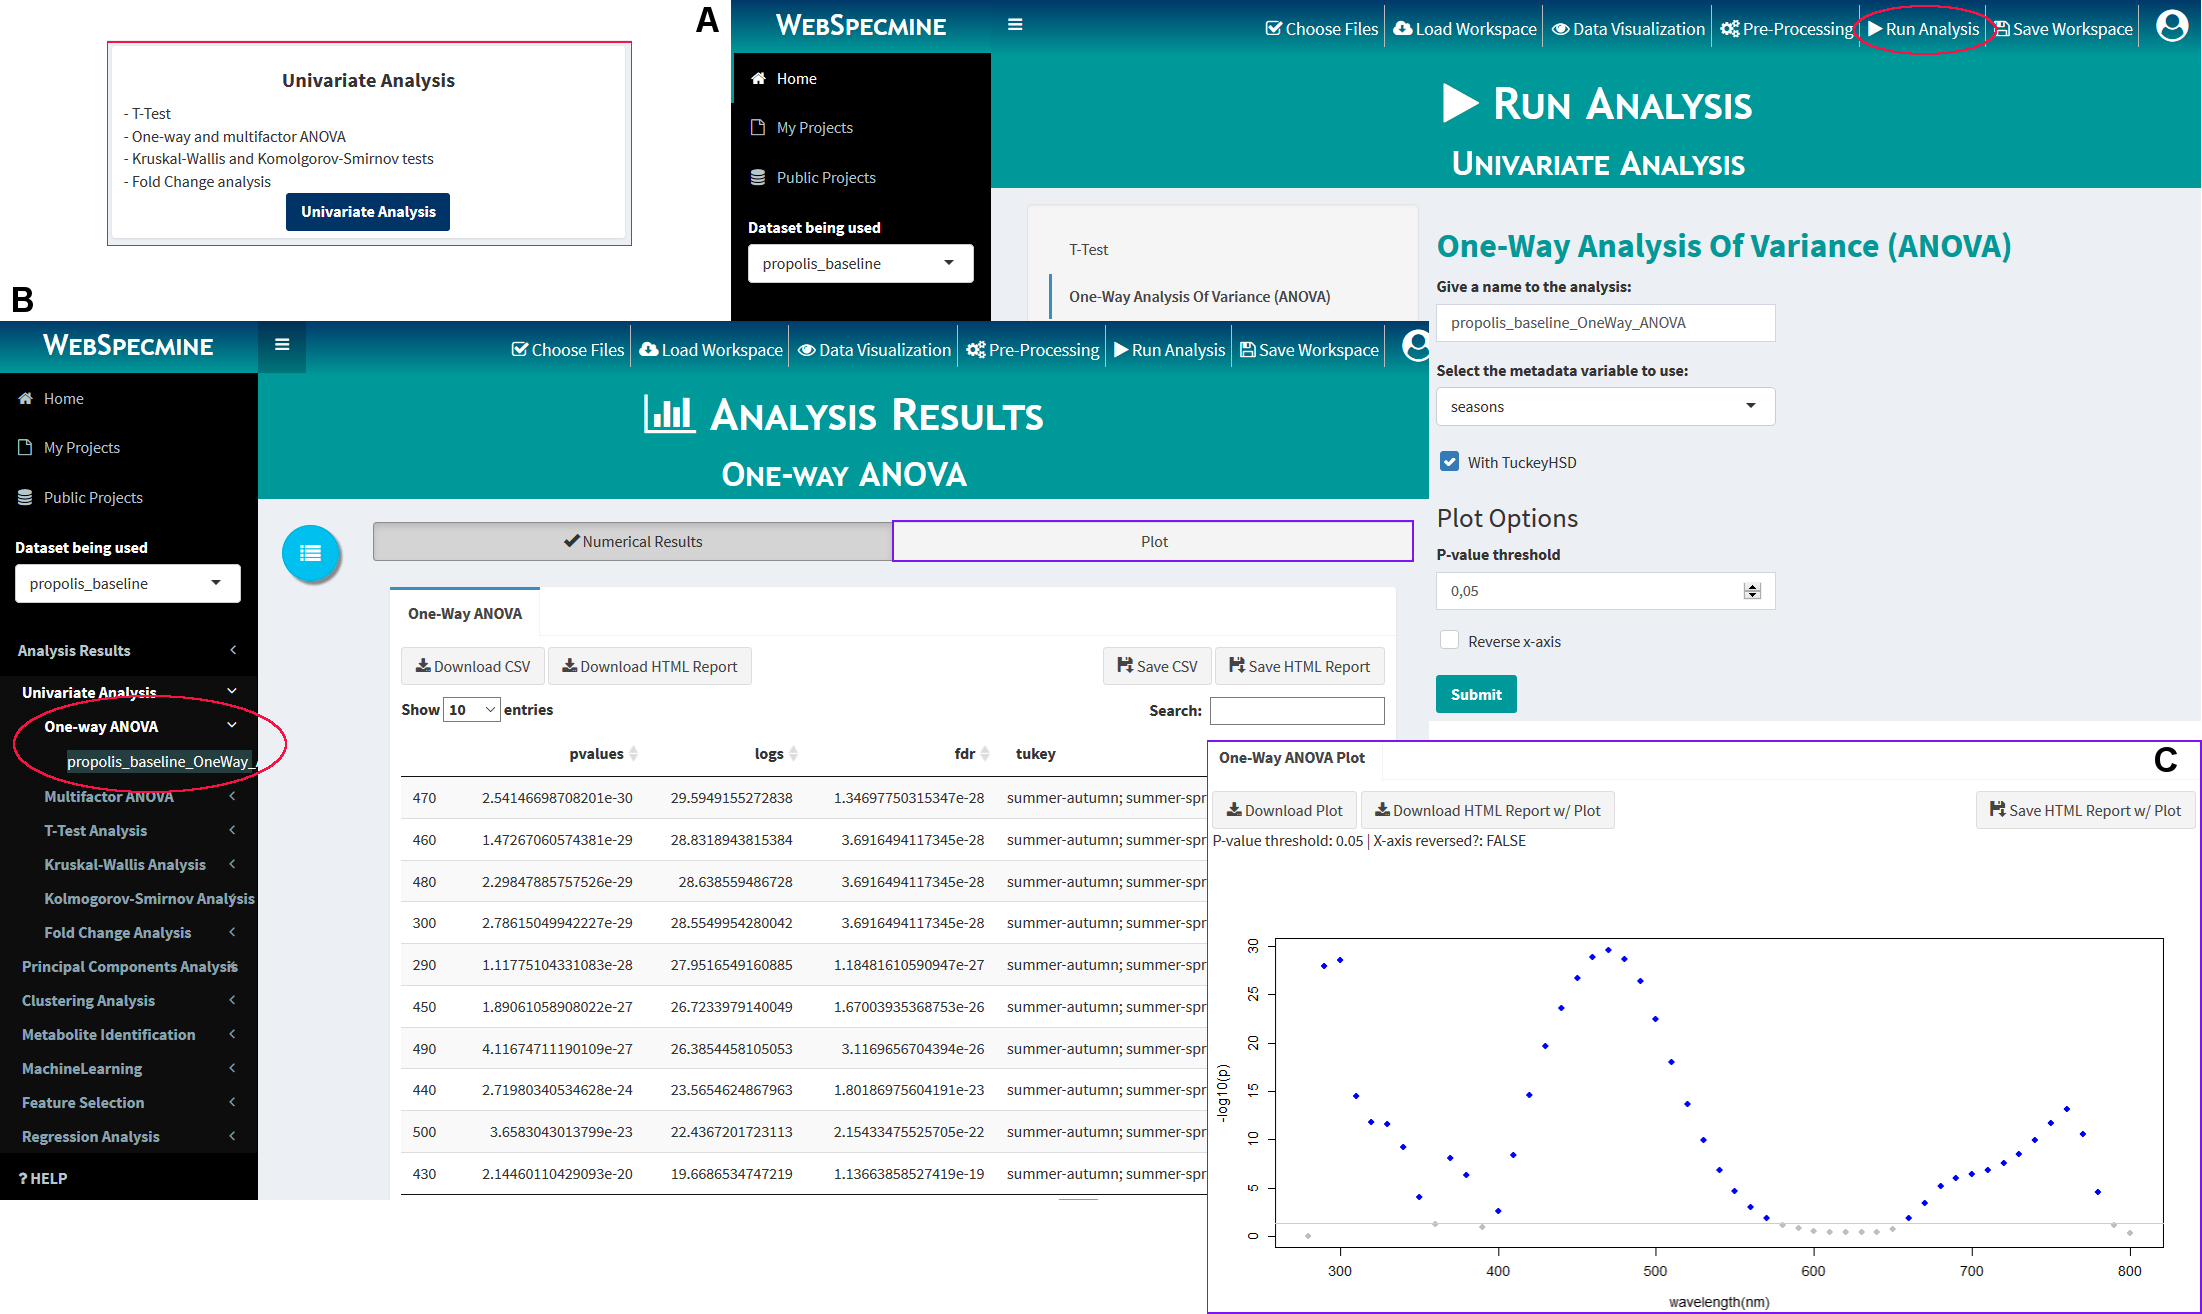
\includegraphics[width=1\linewidth]{Imagens/Propolis/anova}
	\caption{\textit{Run Analysis} page for \gls{anova} (\textbf{A}), and respective results page (\textbf{B}) showing the table results with Tukey's \gls{hsd} for the \textit{seasons} metadata variable. The \gls{anova} plot is also shown, with a defined p-value threshold of 0.05 (horizontal line) (\textbf{C}).}
	\label{propolis_anova}
\end{figure}

The results above indicate that wavelengths between 400 to 500 $\eta m$  appear to have a significant effect on the discrimination of propolis samples over the seasons.

\subsection{Clustering}

Next, we move to multivariate analysis, and an \acrlong{hca} with Euclidean distance measure and complete agglomeration method over the propolis dataset was performed. This type of analysis can be accessed through the \textit{Clustering Analysis} box in the \textit{Run Analysis} page (\autoref{propolis_hca}A). After selecting the desired values for each parameter and pressing \textit{Submit}, the analysis is performed and a new page appears with the analysis results (\autoref{propolis_hca}B). This analysis can be accessed similarly to the previous case.

\begin{figure}[H]
	\centering
	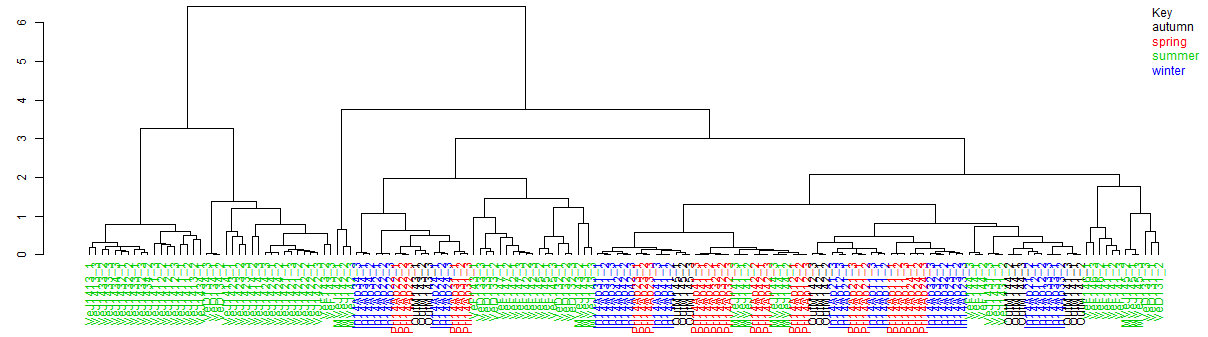
\includegraphics[width=1\linewidth]{Imagens/Propolis/hca}
	\caption{\textit{Run Analysis} page for \gls{hca} (\textbf{A}) and respective results page showing the \gls{hca} dendrogram colored according to the \textit{seasons} metadata variable (\textbf{B}). Euclidean distance and a complete agglomeration method were used.}
	\label{propolis_hca}
\end{figure}

The resulting tree (\autoref{propolis_hca}B) revealed samples discriminated into two main groups, one having samples collected in the four seasons, but with few samples collected in the summer. The other group, however, contains mostly propolis samples produced in the summer, revealing an interesting separation.


\subsection{Principal Components Analysis}

Finally, a \gls{pca} was also performed over the propolis dataset. This analysis can be accessed through the \textit{Principal Components Analysis} box in the \textit{Run Analysis} page (\autoref{propolis_pca}A). 
In this case, centering by mean and scaling by standard deviation was performed, with a pre-defined total of 10 components set. The component importance results are shown in \autoref{propolis_pca}B, also including the pairs plot for the first five components (\autoref{propolis_pca}D) and a 3D scores plot (\autoref{propolis_pca}E), both colored according to the \textit{seasons} metadata variable. \autoref{propolis_pca}C shows the \textit{Make plots} tab for the scree plot. These results may be accessed at any time, similarly to the previous cases.

\begin{figure}[H]
	\centering
	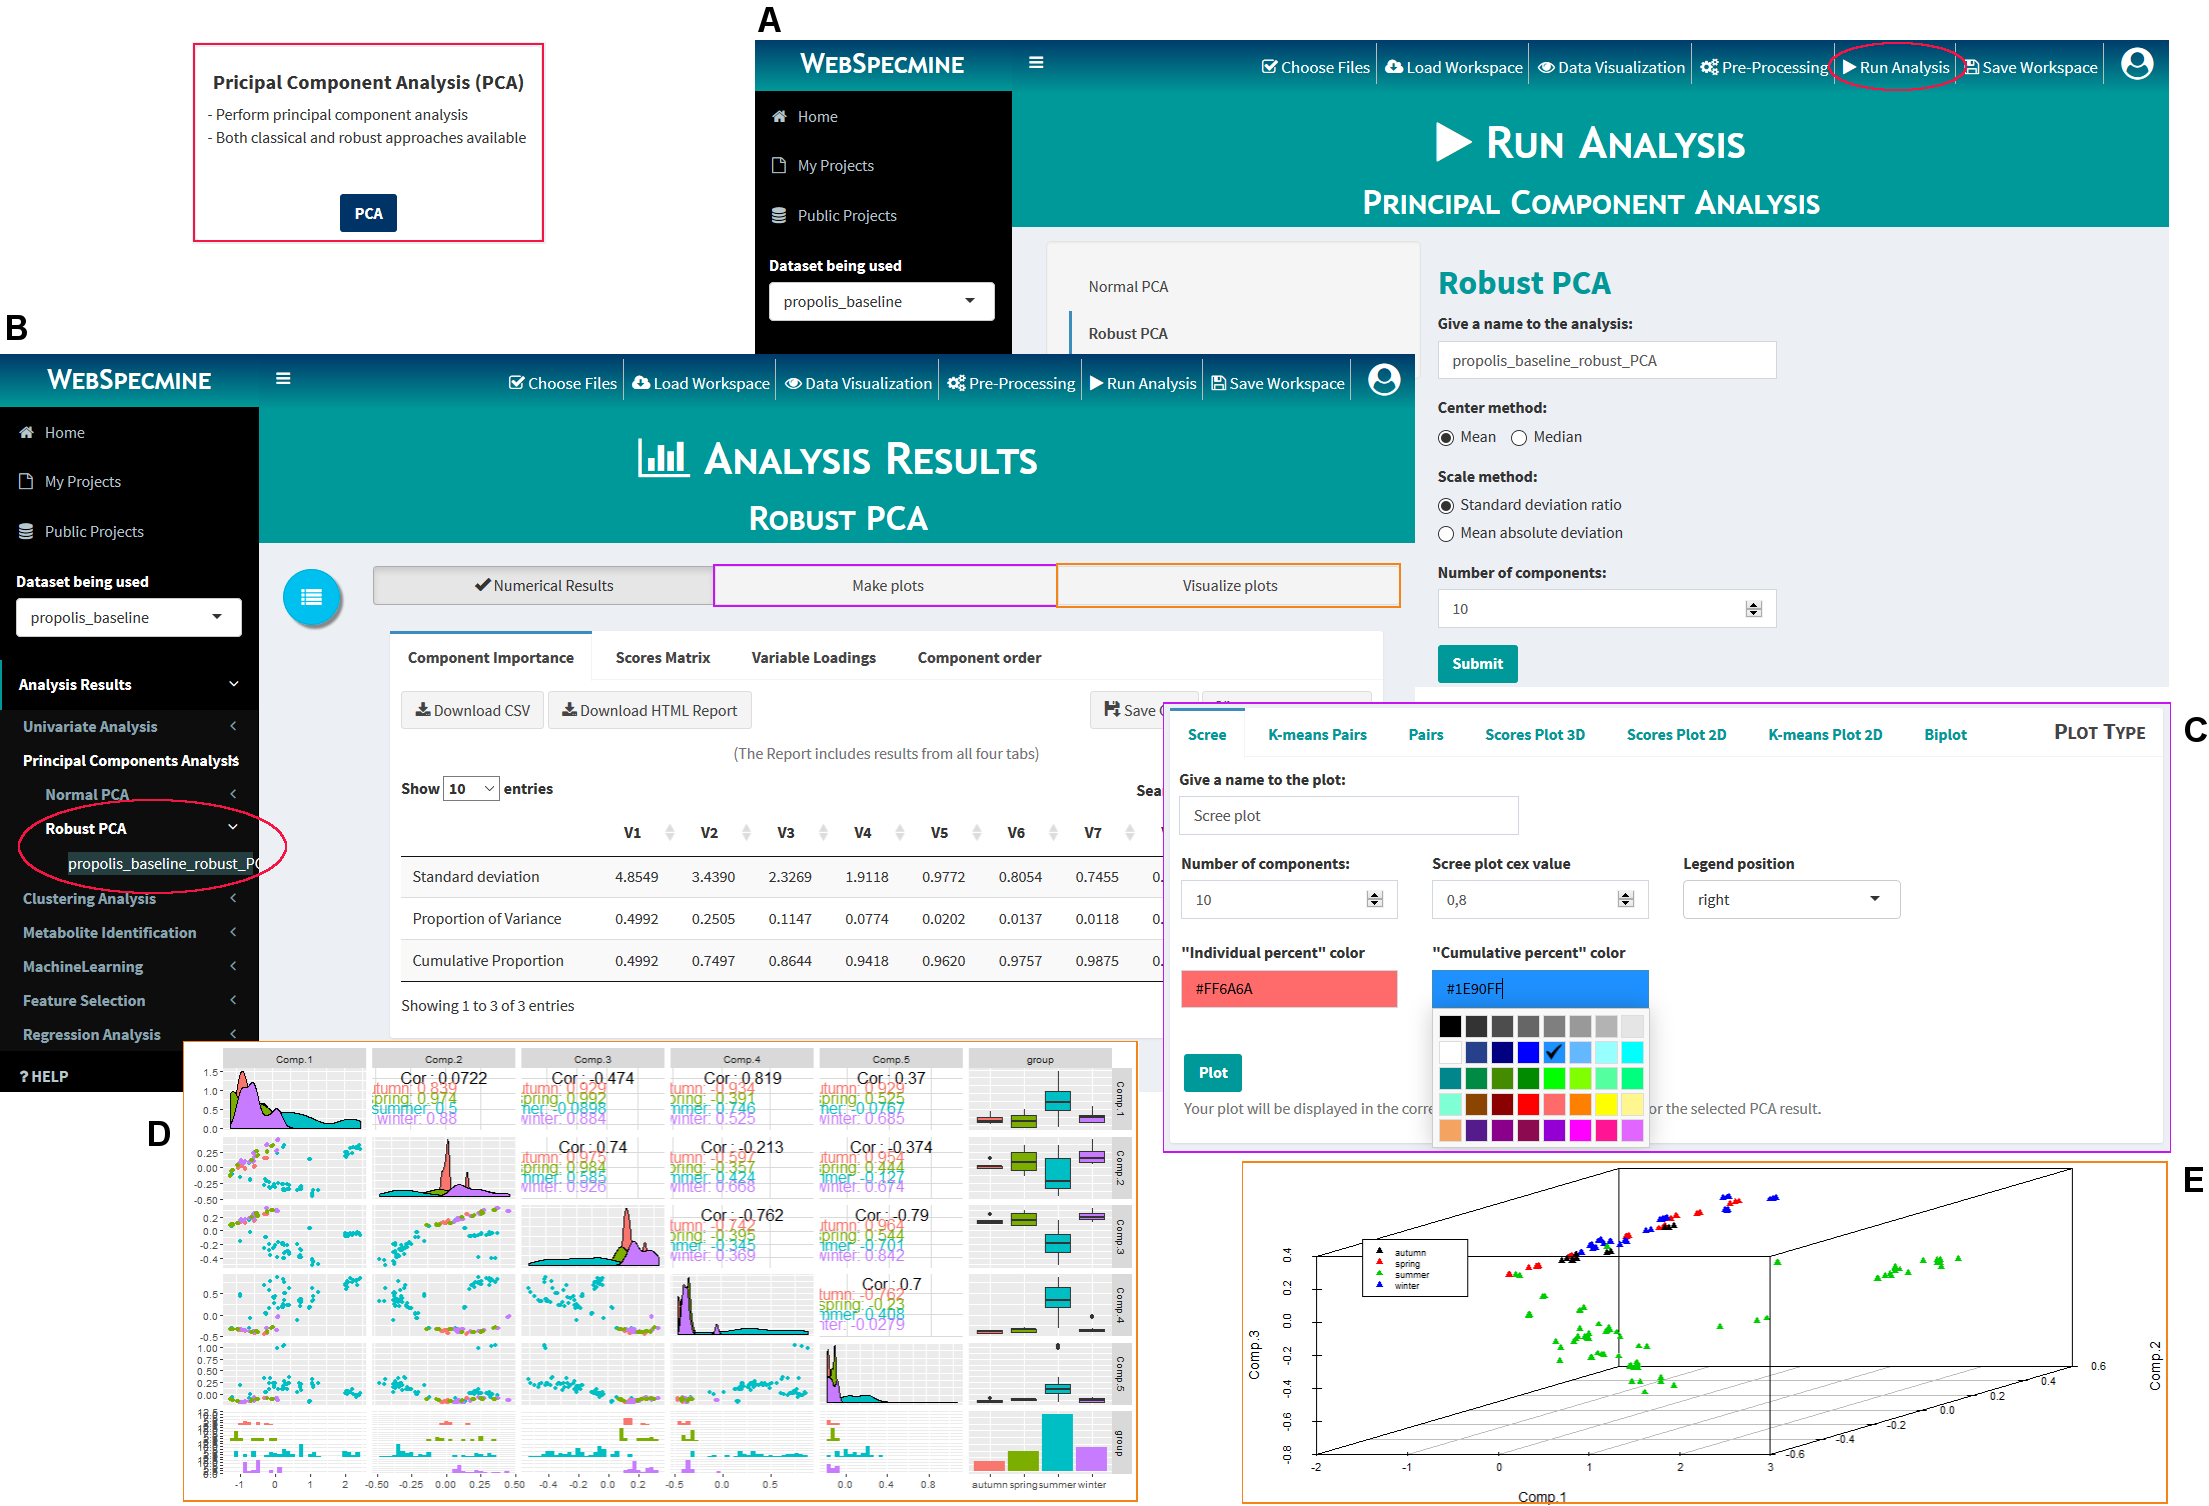
\includegraphics[width=1\linewidth]{Imagens/Propolis/pca}
	\caption{\textit{Run Analysis} page for \gls{pca} (\textbf{A}) and respective results page showing the component importance table (\textbf{B}), the \textit{Make plots} tab for the scree plot (\textbf{C}), and a pairs plot for the first five components (\textbf{D}) and a 3D scores plot (\textbf{E}), both colored according to the \textit{seasons} metadata variable.}
	\label{propolis_pca}
\end{figure}


The first two components PC1 (50\%) and PC2 (25.05\%) explained about 75.05\% of the total variance of the dataset (\autoref{propolis_pca}B). In general, the results of \gls{pca} and \gls{hca} are complementary, by confirming the sample discrimination by seasons into two groups (\autoref{propolis_pca}D, \autoref{propolis_pca}E). 

The raw data and full analysis report performed using the \textit{specmine} package for this study can be accessed at \href{http://darwin.di.uminho.pt/metabolomicspackage/propolis-sj.html}{\nolinkurl{http://darwin.di.uminho.pt/metabolomicspackage/propolis-sj.html}}.




\section{Cassava's post-harvest physiological deterioration}

\subsection{Context}

The \textit{cassava} crop (\textit{Manihot esculenta}) is characterized by its starchy roots, being considered a staple food and animal feed in tropical and sub-tropical areas. As a tropical root crop, it undergoes \acrfull{ppd}, both physiological (or primary deterioration) and microbiological (or secondary deterioration). This process is characterized by the appearance of blue–black streaks in the root vascular tissue, which later spread, causing a more general brown discoloration, unsatisfactory cooking qualities, and adverse taste. \gls{ppd} begins quickly within 24h post-harvest, limiting the marketability of the roots, and they need, therefore, to be consumed shortly after harvesting.

The aim of the present study was to identify and discriminate changes in the chemical and enzymatic composition of cassava genotypes samples during post-harvest deterioration, with the aid of supervised and unsupervised methods of data analysis.

For this, samples with different stages of deterioration were collected, more specifically fresh samples (0 days) and samples with 3 days, 5 days, 8 days and 11 days of deterioration (\gls{ppd}). Additionally, the samples collected were from four different varieties: SCS 253 Sangão (SAN); Branco (BRA); IAC576-70 - \textit{Instituto Agronômico de Campinas} (IAC); and Oriental (ORI). A total of 80 samples were collected (16 samples with 5 replicates each) and the \gls{ir} transmittance spectra recorded over a spectral window from 4000 to 400 $cm^{-1}$ \citep{uarrota2014metabolomics}.


\subsection{Data Loading}

In this case, the dataset will be directly created from the user's local computer files, without the need of authentication, unlike in \autoref{propolis_loading} where it was assumed the user would be logged in and already had the files uploaded in a project on the web platform. The main difference compared to when the user is logged is the fact that there aren't any saved projects ready to import as a dataset, hence the need to import the files containing the data directly from the computer. Additionally, the workspace cannot be saved to later resume the analysis and while reports can still be generated and downloaded, they cannot be saved into the users personal project library. 

To create the dataset, we start by clicking the \textit{New Project} button on the header. A new window appears with fields to upload both data and metadata files and to specify each file's options accordingly (\autoref{cassava_create_project}A). The DX files from this study are stored in a ZIP folder, which can be uploaded directly using the specified field (\autoref{cassava_create_project}B).

\begin{figure}[h]
	\centering
	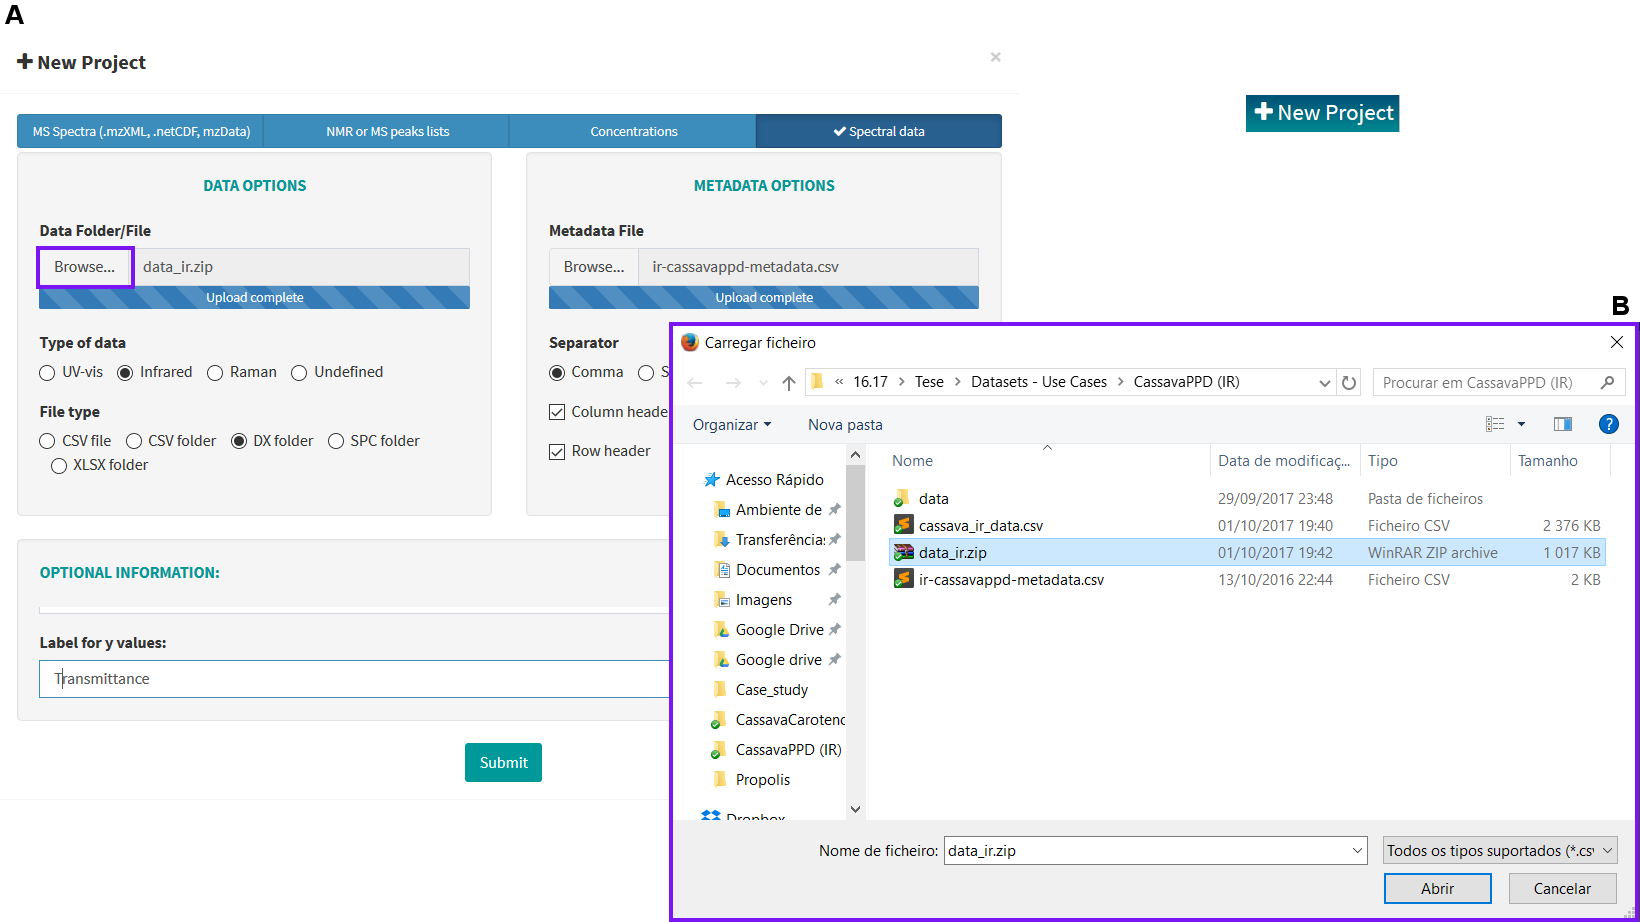
\includegraphics[width=1\linewidth]{Imagens/CassavaPPD/data_load}
	\caption{Upon clicking the \textit{New Project} button on the header a window appears with fields to upload both data and metadata files and to specify each files options accordingly (\textbf{A}). In this case, a zip folder containing DX files is being uploaded (\textbf{B}).}
	\label{cassava_create_project}
\end{figure}


\subsection{Data Overview}

Once the dataset is created, its information can be easily accessed in the \textit{Data Visualization} page. In \autoref{cassava_data_overview}, the summary of the propolis dataset, along with the spectra plot colored by the \textit{varieties} metadata variable and the first 11 rows of the metadata table are shown. The \gls{ir} dataset has 3 metadata variables, a total of 80 samples and about 3735 data points, with no missing values.

\begin{figure}[h]
	\centering
	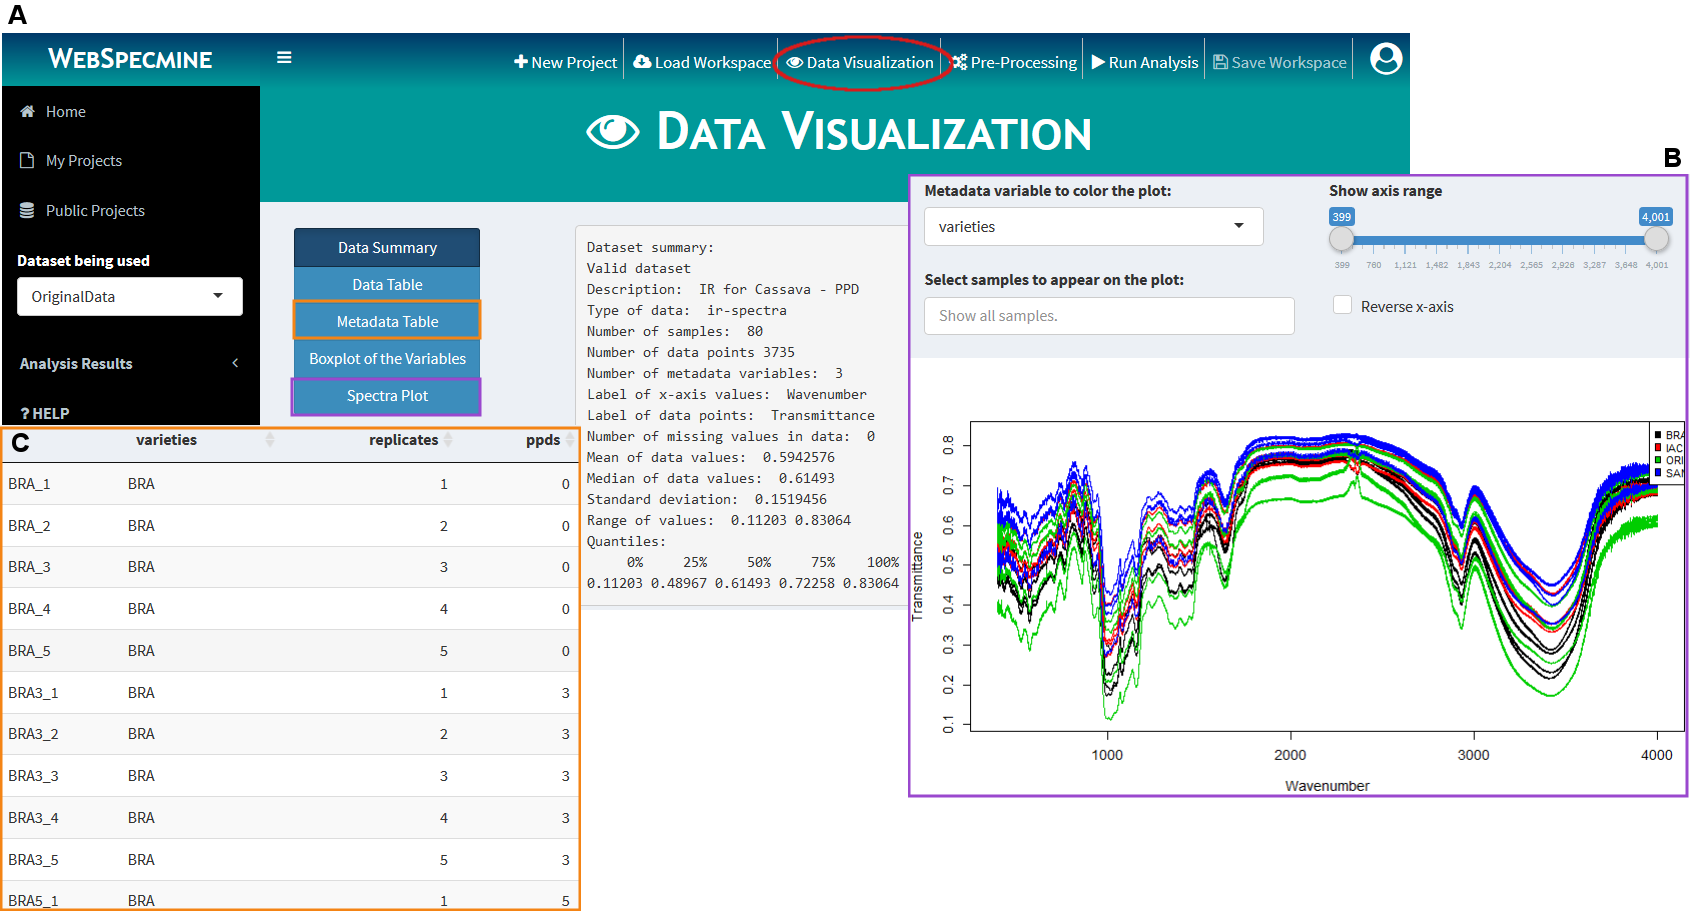
\includegraphics[width=1\linewidth]{Imagens/CassavaPPD/data_overview}
	\caption{The \textit{Data Visualization} page showing the dataset summary (\textbf{A}), the spectra plot colored by the \textit{varieties} metadata variable (\textbf{B}) and the first 11 rows of metadata table (\textbf{C}).}
	\label{cassava_data_overview}
\end{figure}


\subsection{Pre-processing}

The pre-processing methods used in this study consisted in converting the \textit{ppd} metadata variable to factor, the aggregation of replicates and applying smoothing interpolation. All these methods can be easily applied over the dataset on the \textit{Pre-Processing} page by going the respective method box and, after selecting the parameters accordingly, click the button on the box to apply the selected method. 
As before, a name must be given to the new dataset and the process is done (\autoref{cassava_preprocessing}).

\begin{figure}[H]
	\centering
	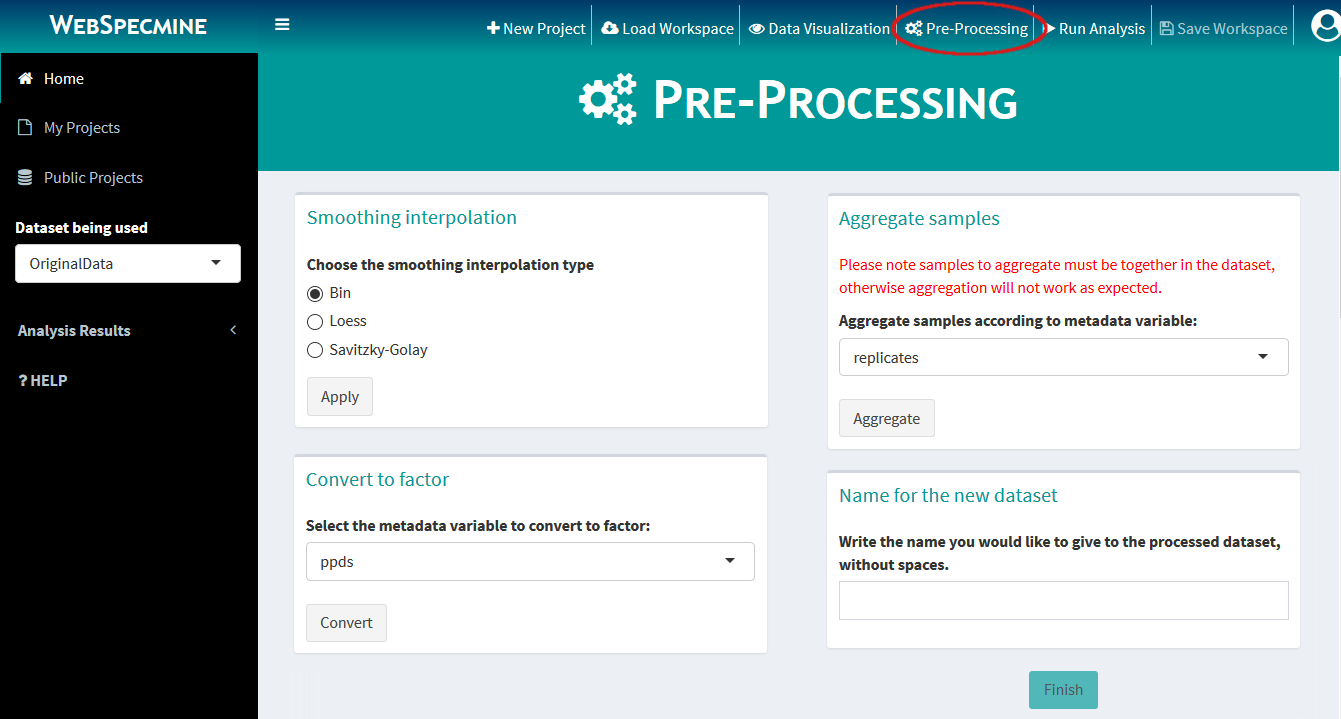
\includegraphics[width=0.8\linewidth]{Imagens/CassavaPPD/preprocessing}
	\caption{The \textit{Pre-Processing} page emphasizing the boxes for smoothing interpolation, conversion to factor and sample aggregation. Please note the image was edited to emphasize the pre-processing methods used in this example.}
	\label{cassava_preprocessing}
\end{figure}


From the \textit{Data Visualization} page the effects of the applied pre-processing methods are noticeable (\autoref{cassava_summary_preprocessing}A). The dataset now has 16 samples, 1868 data points and 2 metadata variables. The \textit{ppd} metadata variable, as a factor, can now be used to color the plot (\autoref{cassava_summary_preprocessing}B).

\begin{figure}[H]
	\centering
	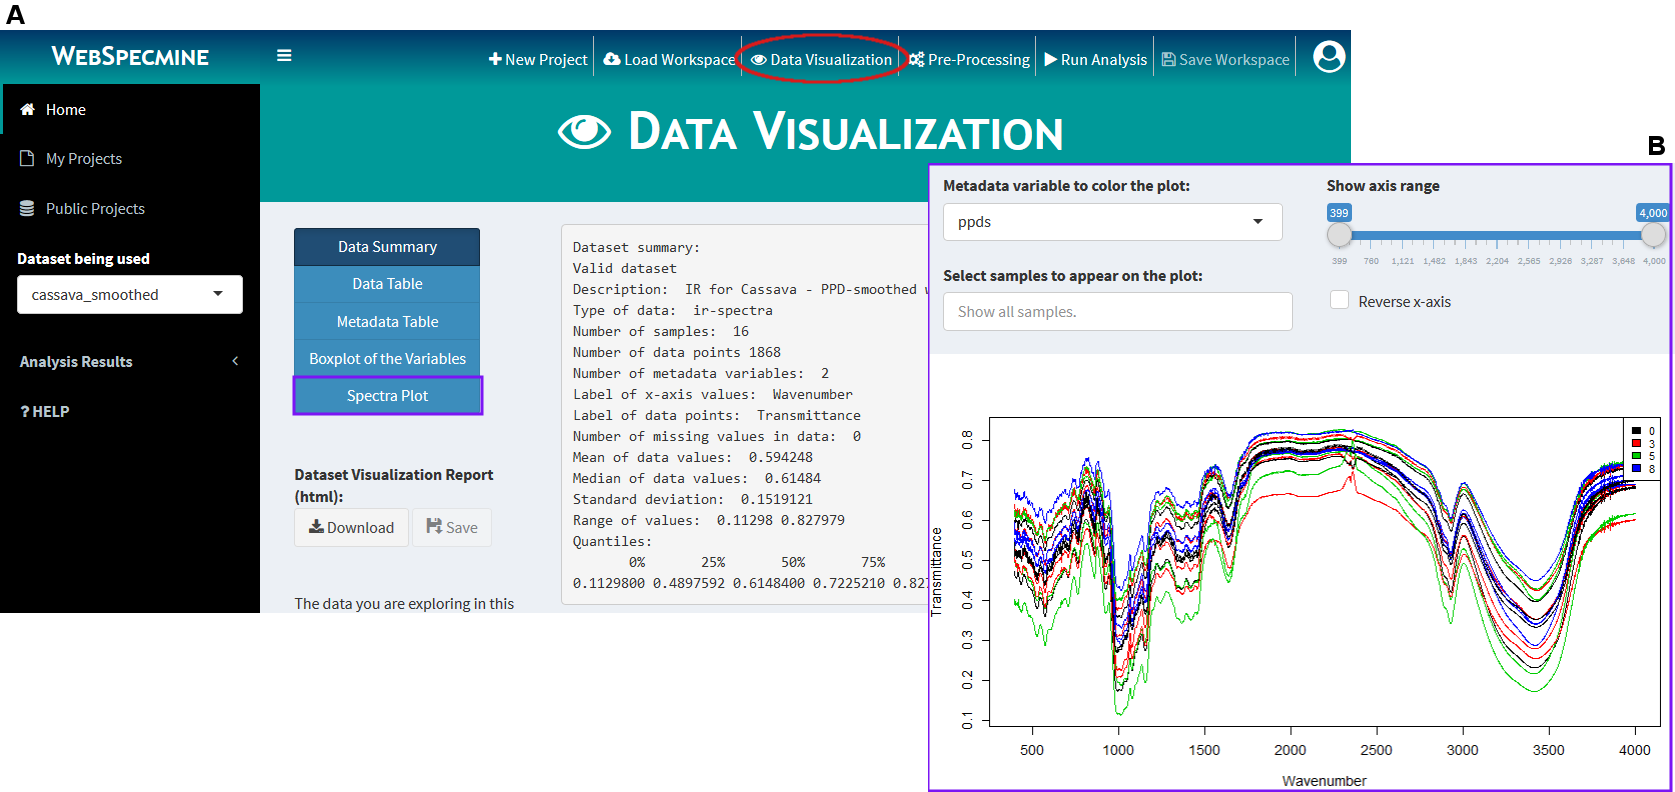
\includegraphics[width=1\linewidth]{Imagens/CassavaPPD/data_overview_preproc}
	\caption{The \textit{Data Visualization} page showing the dataset summary (\textbf{A}) and the spectra plot colored by the \textit{ppd} metadata variable (\textbf{B}) after data pre-processing.}
	\label{cassava_summary_preprocessing}
\end{figure}


\subsection{Principal Components Analysis}

A \gls{pca} was performed over the cassava dataset. This analysis can be accessed through the \textit{Principal Components Analysis} box in the \textit{Run Analysis} page (\autoref{propolis_pca}A). The data was both scaled and centered for this analysis. The component importance results are shown in \autoref{cassava_pca}B, also including the pairs plot for the first five components (\autoref{propolis_pca}C), the K-means pairs plot for the first 5 components (3 clusters) (\autoref{propolis_pca}D) and the distribution of the 16 samples on the first and second \gls{pca} components on a scored plot using the \textit{ppd} metadata variable (\autoref{propolis_pca}E). 


\begin{figure}[H]
	\centering
	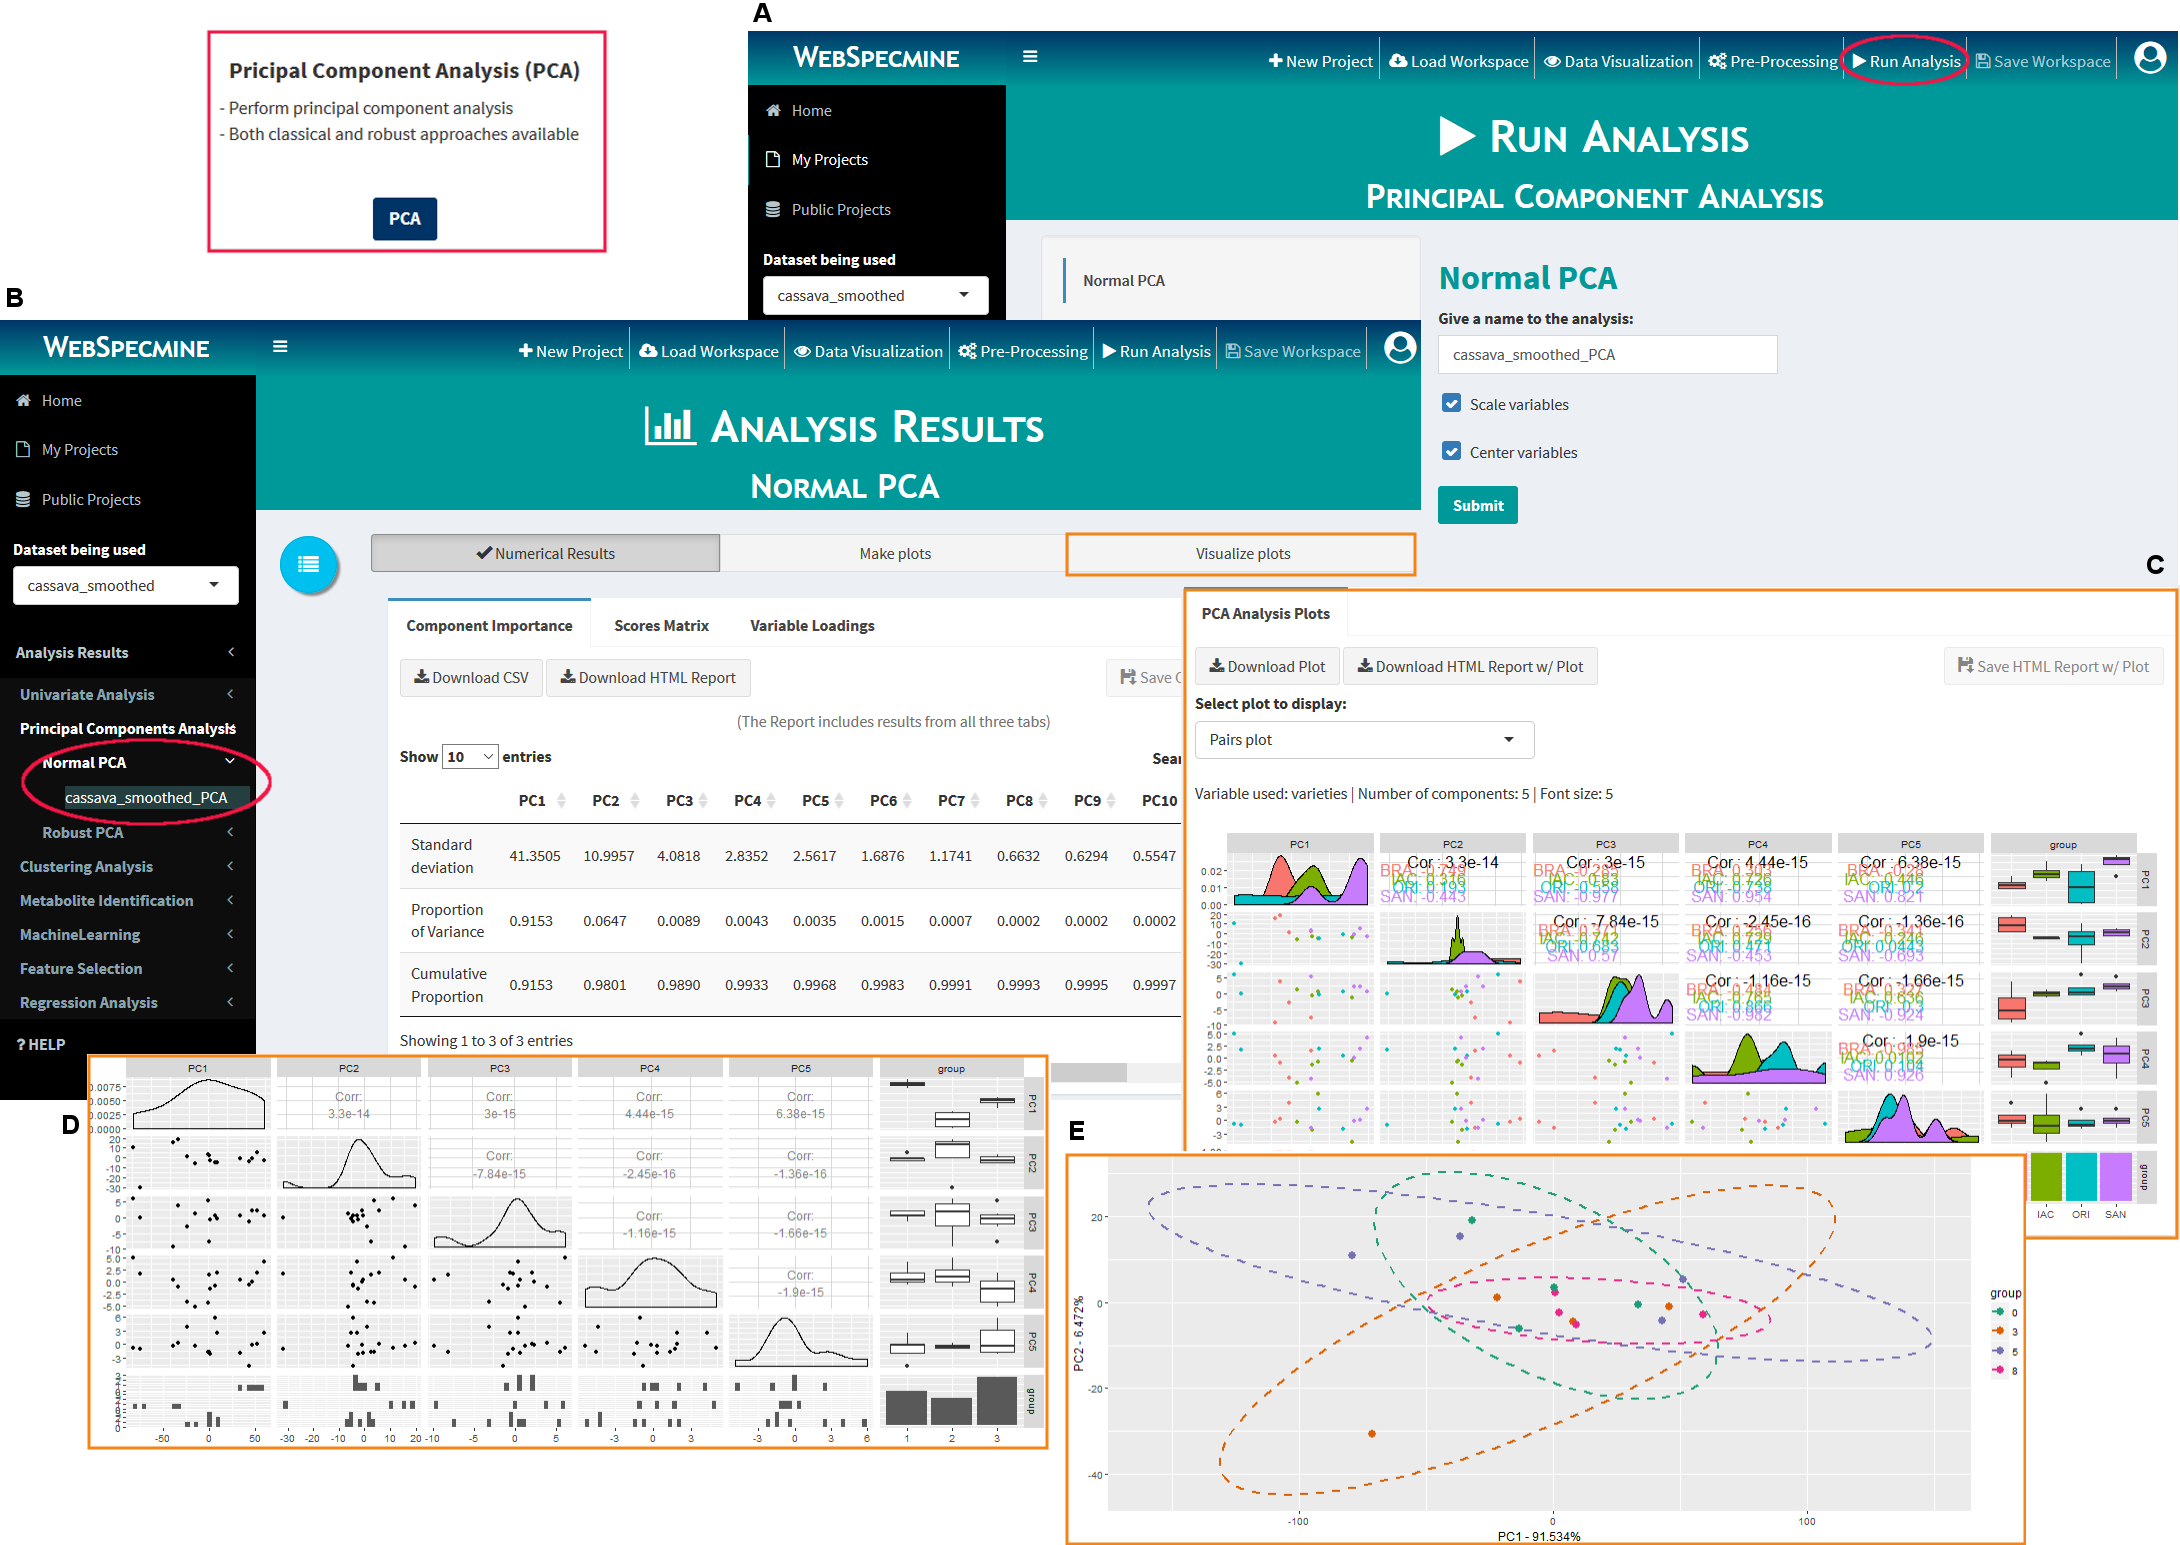
\includegraphics[width=1\linewidth]{Imagens/CassavaPPD/pca}
	\caption{\textit{Run Analysis} page for \gls{pca} (\textbf{A}) and respective results page showing the component importance table (\textbf{B}), a pairs plot for the first five components (\textbf{C}), a k-means plot for the first five components (3 clusters) (\textbf{D}) and a 2D scores plot for the \textit{ppd} metadata variable (\textbf{E}).}
	\label{cassava_pca}
\end{figure}

The total variance of the data explained by the \gls{pca} model built was 98.01\%, with 91.63\% from PC1 and 6.47\% from PC2 (\autoref{cassava_pca}B). A visible separation between ORI and BRA (susceptible and tolerant \gls{ppd} genotypes, respectively) is shown, although some overlap of the samples of most genotypes was observed (\autoref{cassava_pca}C). The scores plot showed sample overlapping using the \textit{ppd} metadata variable (\autoref{cassava_pca}E).



\subsection{Correlation Analysis}

A correlation analysis was also performed over the cassava dataset. This type of analysis can be accessed through the \textit{Regression Analysis} box in the \textit{Run Analysis} page. For this analysis the Pearson correlation method was chosen, calculating the correlation between samples (\autoref{cassava_correlation}A). \autoref{cassava_correlation}B shows the resulting correlation matrix, with the corresponding generated heatmap represented in \autoref{cassava_correlation}C.


\begin{figure}[H]
	\centering
	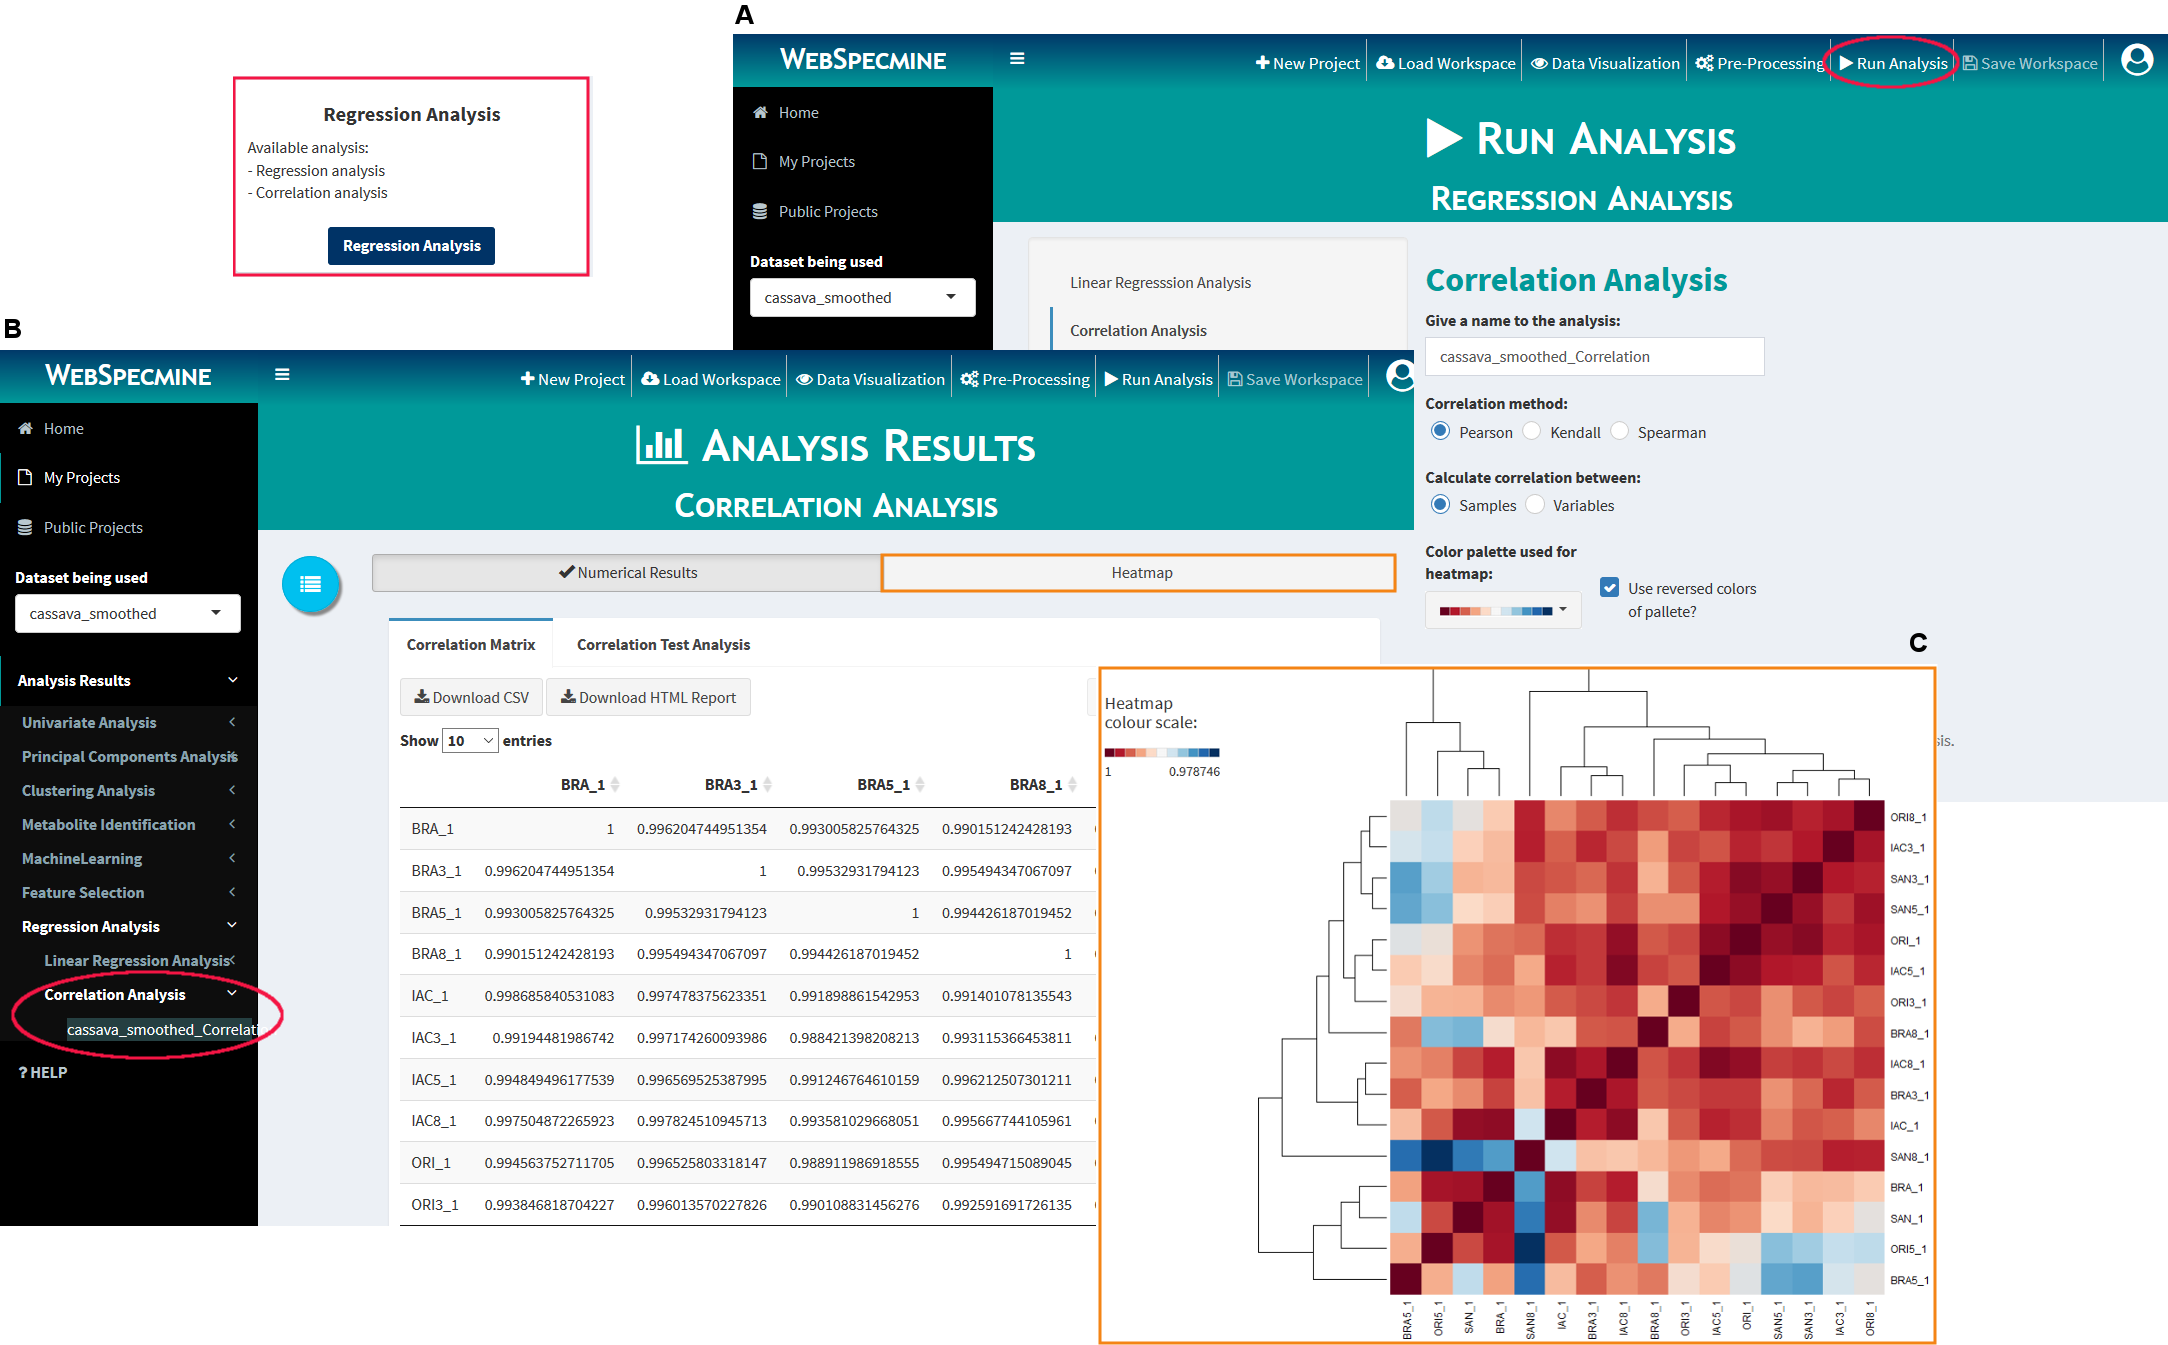
\includegraphics[width=1\linewidth]{Imagens/CassavaPPD/correlation}
	\caption{\textit{Run Analysis} page for correlation analysis (\textbf{A}) and respective results page showing the correlation matrix (\textbf{B}) and resulting heatmap correlating samples (\textbf{C}).}
	\label{cassava_correlation}
\end{figure}

The heatmap generated suggests most samples are positively correlated (\autoref{cassava_correlation}C).


\subsection{Feature Selection}

Next, a feature selection approach was performed over the dataset. To access this type of analysis, simply select the \textit{Feature Selection} box in the \textit{Run Analysis} page. Here, the \gls{rfe} method was selected, choosing random forests model to fit the data and the \textit{varieties} metadata as response variable. A 10-fold cross-validation was selected (\autoref{cassava_feature_selection}A), with 5 repetitions. In \autoref{cassava_feature_selection}B, the feature selection results are displayed, as well as the plot with the performance profile in \autoref{cassava_feature_selection}C. 


\begin{figure}[H]
	\centering
	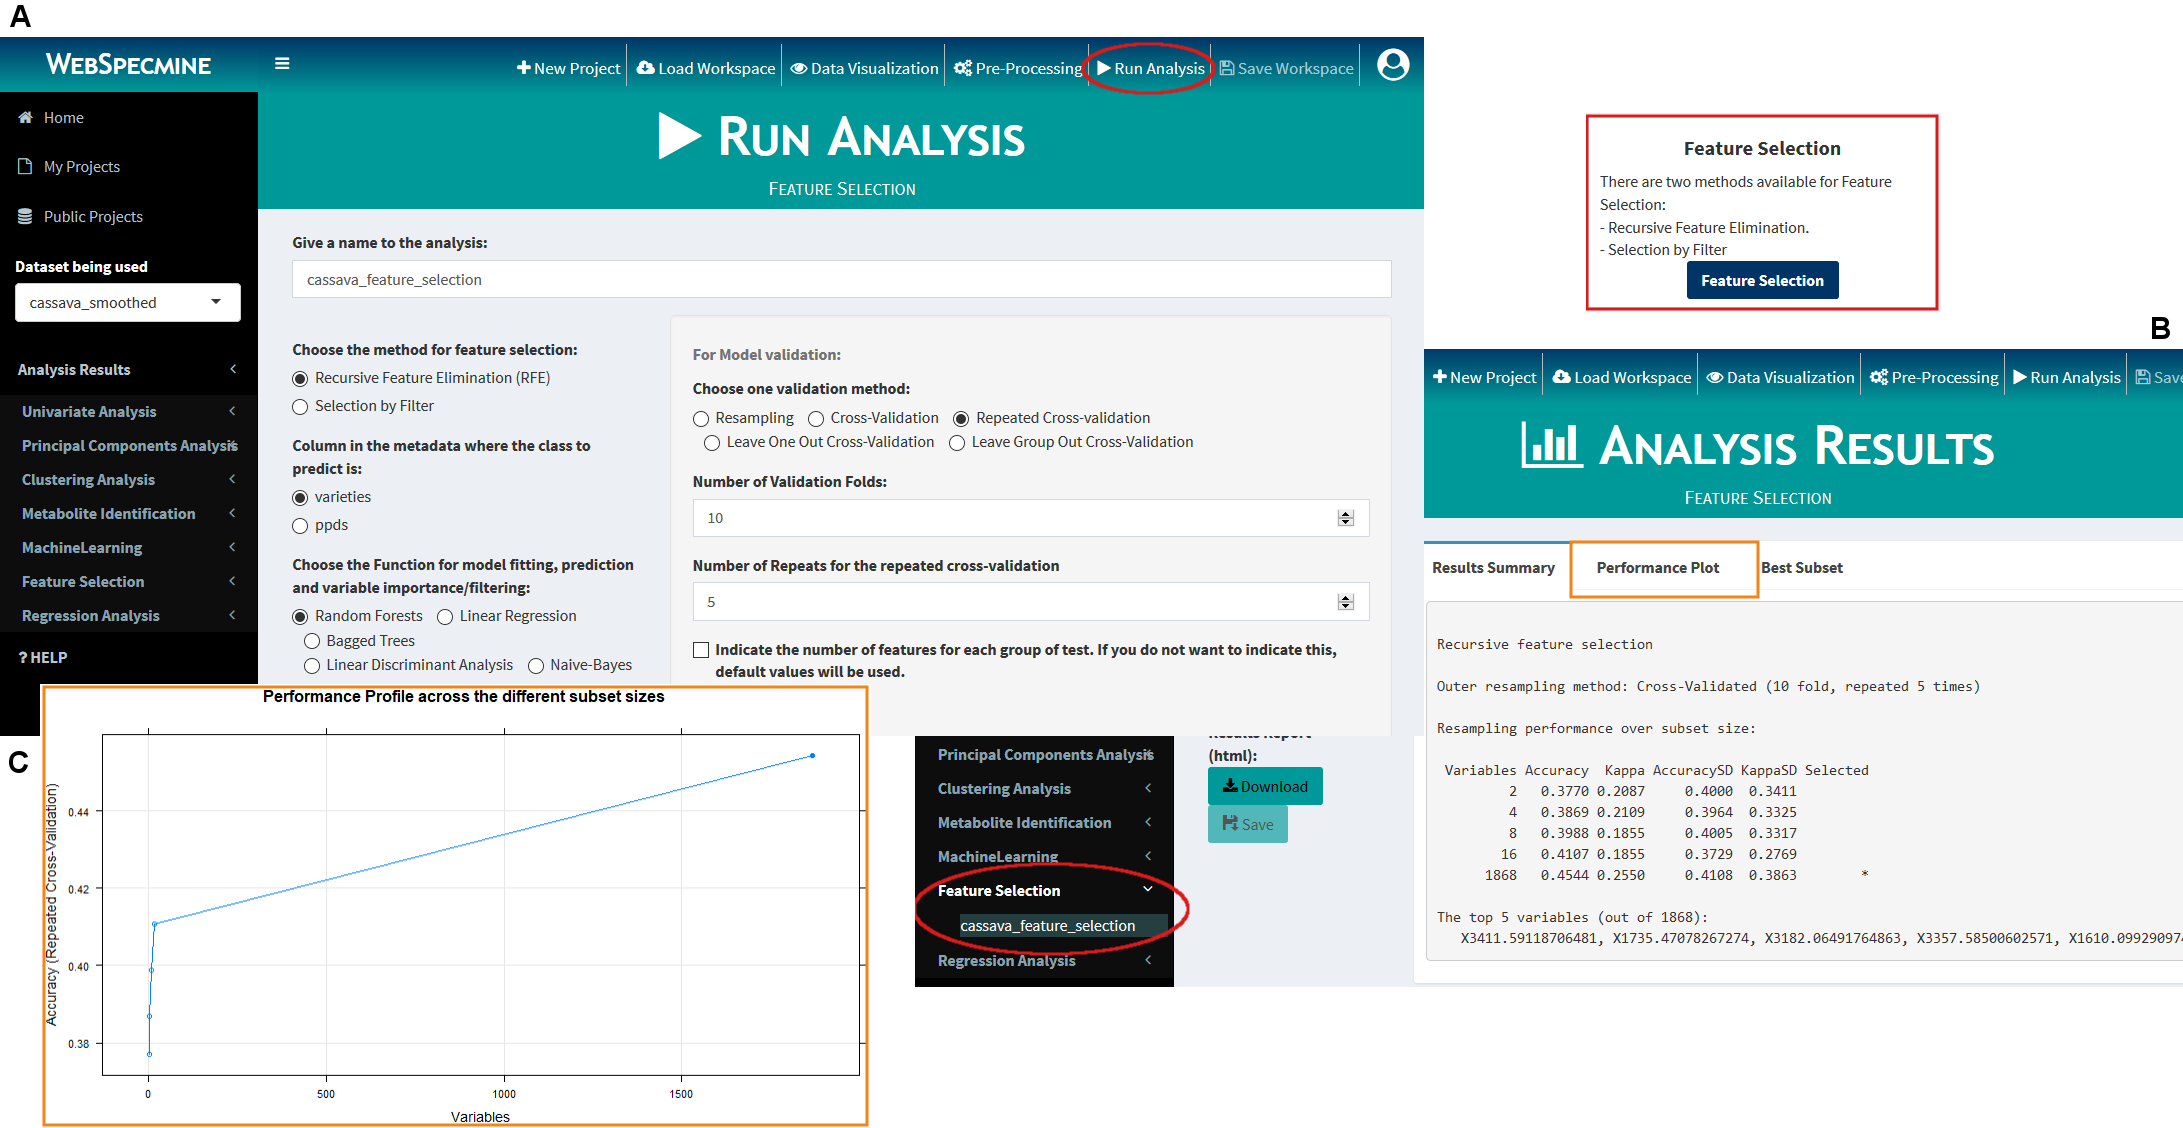
\includegraphics[width=1\linewidth]{Imagens/CassavaPPD/feature_selection}
	\caption{\textit{Run Analysis} page for feature selection analysis (\textbf{A}), and respective results page showing the performance metrics (\textbf{B}) and plot with the performance profile (\textbf{C}).}
	\label{cassava_feature_selection}
\end{figure}

The results above indicate that there is no improvement in cross-validation performance by performing feature selection, with the best accuracy being achieved when using the entire set of features.


\subsection{Machine Learning}

Finally, a machine learning analysis was performed. This type of analysis can be accessed through the \textit{Machine Learning} box in the \textit{Run Analysis} page. In this analysis, the \gls{pls} model was chosen to fit the data, using the \textit{ppd} metadata variable for class prediction. A 10-fold cross-validation was selected, with accuracy as selected performance metric (\autoref{cassava_machine_learning}A). \autoref{cassava_machine_learning}B displays the analysis' performance metrics for the \gls{pls} model, while \autoref{cassava_machine_learning}C shows the full results from the tuning parameters for this model, with the variable importance table shown in \autoref{cassava_machine_learning}D.


\begin{figure}[H]
	\centering
	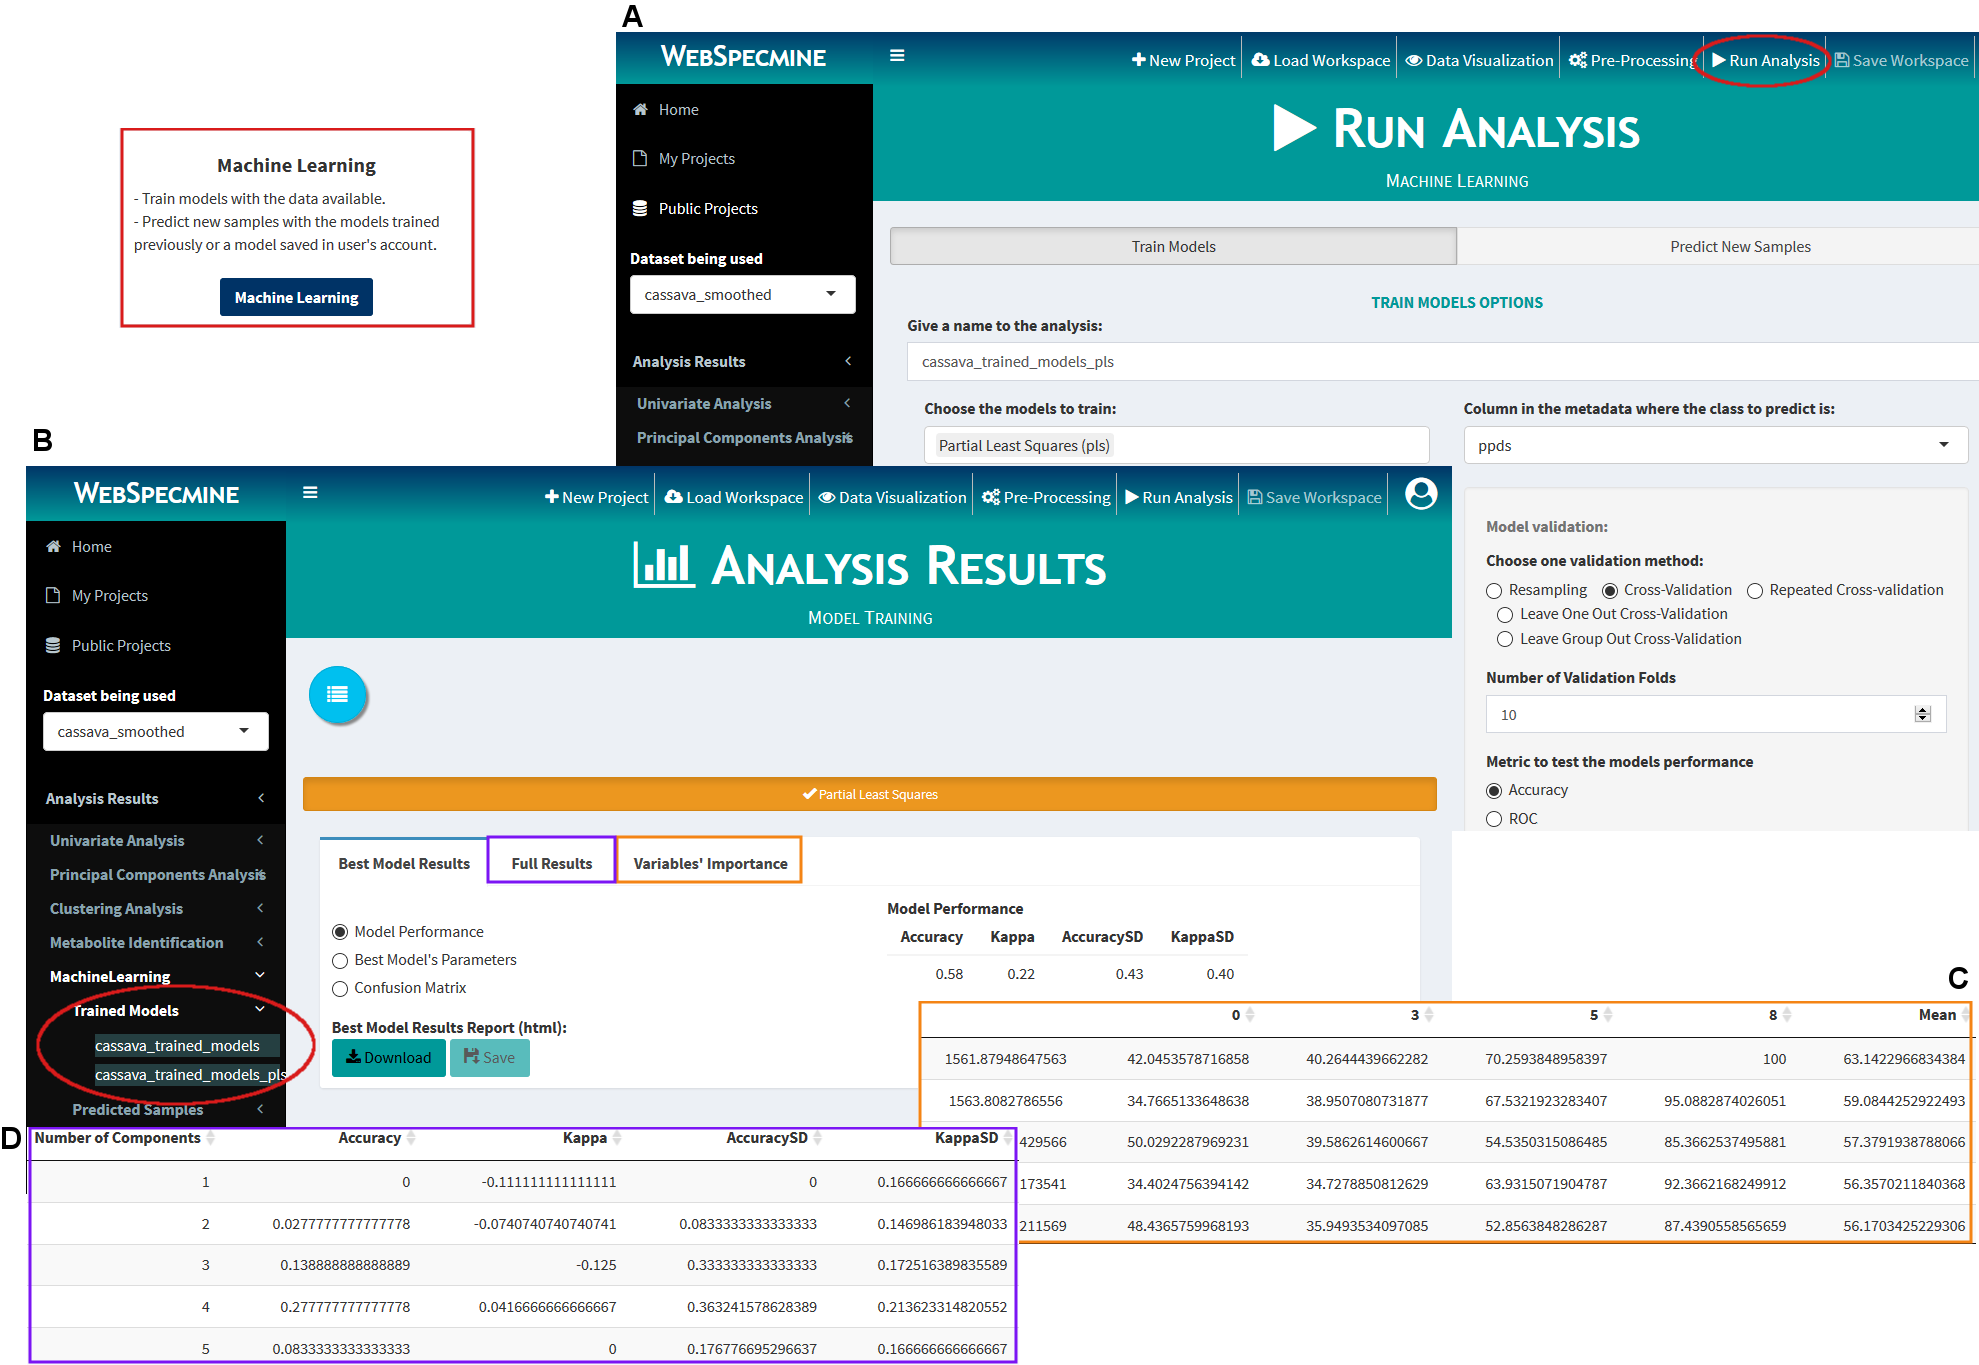
\includegraphics[width=1\linewidth]{Imagens/CassavaPPD/ml}
	\caption{\textit{Run Analysis} page for machine learning analysis (\textbf{A}) and respective results page showing the performance metrics for the \gls{pls} model (\textbf{B}), the full results from the tuning parameters for this model (\textbf{C}) and the variable importance table (\textbf{D}).}
	\label{cassava_machine_learning}
\end{figure}


The machine learning results show that the \gls{pls} model accurately predicted the samples' class about 58\% of the times, with the most relevant features for the classification being the wavenumbers around 1560 $cm^{-1}$.

The full analysis reports performed using the \textit{specmine} package for this study can be accessed at \href{http://darwin.di.uminho.pt/metabolomicspackage/cassava.html}{\nolinkurl{http://darwin.di.uminho.pt/metabolomicspackage/cassava.html}}.





	
	
	% CHAPTER - Case Studies
	
	
\chapter{Case study: characterizing carotenoid contents in cassava} \label{case_study}

The aim of this chapter is to present a more elaborate case study, using real data from one of the the host groups (Universidade Federal de Santa Catarina, Brazil), providing a meaningful pipeline with the ability to demonstrate the application's features, as well as the ones of the underlying \textit{specmine} package. This case study consists in the chemometric characterization of the carotenoid content in cassava roots tissue, using \gls{uv}, CIELAB data and a \acrfull{llf} of the two.

Unlike the previous ones, the author was involved in this study since the beginning, being one of the authors of the respective publication, accepted and presented at the 11$^{th}$ International Conference on \acrfull{pacbb} during the development of this thesis \citep{moresco2017classification}. The extended version of the published study has been accepted for publication in the \textit{Journal of Integrative Bioinformatics}.


\section{Introduction}

Cassava is the commonly used term to designate the \textit{Manihot esculenta} species. This tuberous-root plant species offers a wide variety of agronomic advantages, being resilient to droughts, inexpensive, resistant to major diseases and pests, easy to grow and having flexible harvest times, allowing farmers to harvest the roots as needed. It is, therefore, a valuable source of energy for people living in the poorest regions. However, cassava roots are a poor source of provitamin A carotenoids, whose deficiency is a major problem in such regions \citep{la2013biofortified, sanchez2014prediction}. 

Carotenoids are one of the most important natural pigments, having already been recognized benefits of carotenoid consumption, such as the diminished risk of several degenerative disorders, including various types of cancer, cardiovascular or ophthalmological diseases, as well as their preventive effect associated with their antioxidant activity, protecting cells and tissues from oxidative damage \citep{stahl2003antioxidant}. However, only vitamin A precursors $\beta$-carotene, $\alpha$-carotene and $\beta$-cryptoxanthin represent the major sources of carotenoids in the human diet.

With a broad range of colors, varying from yellow to dark-red, carotenoids confer color to many plant leaves, fruits and flowers, as well as birds, insects, fish, and crustaceans. The color of cassava's starchy root, which can vary from white to red, is strongly correlated to the presence and contents of several carotenoid pigments and their associations \citep{sanchez2006reduction}. However, the possibility of adopting the color of roots as an indirect criterion for selection of higher carotene content is questionable, since color is a characteristic of difficult visual evaluation. Thus, the use of a standardized color measurement technique is of most importance.

The CIELAB color technique was adopted by the \gls{cie} and is based on the Lab color space, which describes mathematically all perceivable colors in three dimensions: L* for lightness and a* and b* for the color opponents green-red and blue-yellow. The values of these three variables are usually absolute, with the L* value representing the darkest black at L* = 0, and the brightest white at L* = 100. On the other hand, the a* value represents red and green opponents at positive and negative values, while the b* value represents yellow and blue opponents at positive and negative values, respectively \citep{brockes1982evaluation, schanda2007colorimetry}. A visual representation of the CIELAB color space is shown in \autoref{cielab}.

\begin{figure}[h]
	\centering
	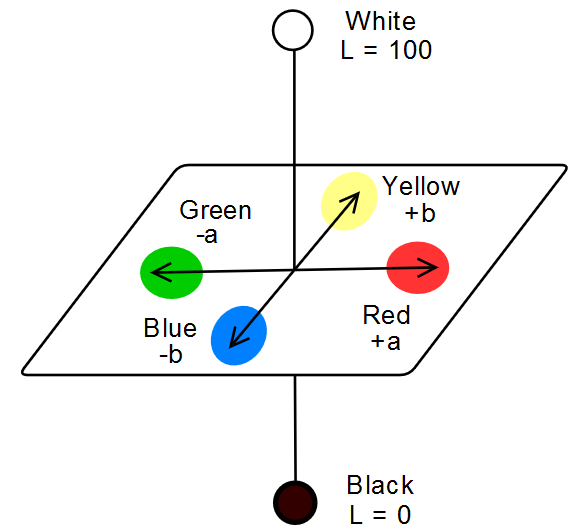
\includegraphics[width=0.4\linewidth]{Imagens/Case_study/cielab}
	\caption{Representation of the CIE L* a* b* color space.}
	\label{cielab}
\end{figure}

Currently, CIELAB is the most used system for quantitative color description of an object, given its uniformity, ease of acquisition, very low cost and device independence. Considering that this technique facilitates the acquisition of measurements directly on the field, while also avoiding the degradation of the compounds, it becomes an appealing approach in comparison to traditionally used methods such as \gls{hplc} or \gls{uv}. The CIELAB color technique has been applied for instance in the unique identification of skin color for clinical and scientific purposes \citep{weatherall1992skin}, and as an optimal color design approach for transforming patients' perception into color elements \citep{liu2014optimal}.

Combining \gls{uv} and CIELAB colorimetric data, the aim of the present case study is to validate a quantification method for carotenoid content estimation in roots of \textit{M. esculenta}, assuming that the statistical and machine learning techniques can correlate these data types, to ultimately detect genotypes of \textit{M. esculenta} with high contents of carotenoids. Importantly, this study provides tools that can support the plant-breeding program at Epagri (Agricultural Research Company and Rural Extension of the State of Santa Catarina, \href{http://www.epagri.sc.gov.br/}{\nolinkurl{http://www.epagri.sc.gov.br/}}) that aims to obtain genotypes with high levels of pro-vitamin A carotenoids and superior nutritional traits.


\section{Materials and Methods} \label{MM}

\subsection{Selection of cassava genotypes} \label{cassava_gen}

Fifty root samples of \textit{M. esculenta} genotypes harvested in 2015/2016 season from the Epagri's germplasm bank (Urussanga Experimental Station, 28$^{\circ}$31'18''S, 49$^{\circ}$19'03''W, Santa Catarina, southern Brazil) were used in this study due to their economic and social importance.

All genotypes were cultivated under the same soil, climatic conditions and agricultural treatments. Importantly, the investigated genotypes were pre-selected according to their relevance for biofortification projects, due to the presence of carotenoids with provitamin A activity and lycopene (visual selection), low levels of cyanogenic glycosides and suitable agronomic traits (e.g., high yield, resistance to drought and to pests and diseases), being widely cultivated in southern Brazil. The fifty genotypes from the germplasm bank were, in fact, indicated by the Epagri plant breeder team given the samples' preference by local small farmers for commercial production due to their physiochemical variability.  


\subsection{Carotenoid extraction and quantification} \label{carot_quant}

Carotenoids were extracted from fresh cassava roots as described in  \cite{rodriguez2004harvestplus} using an Ultra-Turrax (Janke \& Kunkel IKA - T25 basic) and mixture of acetone: petroleum ether (v/v) as extraction solution.

The absorbances of the organosolvent extracts were then recorded on an \gls{uv} spectrophotometer (Gold Spectrum lab 53 \gls{uv} spectrophotometer, BEL photonics, Brazil) using a spectral window from 200 to 700 $\eta m$. Aliquots (10 $\mu l$) of the extracts were also injected into a liquid chromatograph (LC-10A Shimadzu) system equipped with a C18 reversed-phase column (Vydac 201TP54, 250$mm$ x 4.6$mm$, 5$\mu m$ $\phi$, 35$^{\circ}$C) coupled to a pre-column (C18 Vydac 201TP54, 30$mm$ x 4.6$mm$, 5$\mu m$ $\phi$) and a spectrophotometric detector (450 nm). A mixture of methanol: acetonitrile (90:10, v/v) was used for elution at a flow rate of 1 $mL$/min. The identification and quantification of compounds of interest was carried out via co-chromatography and comparison of retention times of samples with those of standard compounds (Sigma–Aldrich, USA) under the same experimental conditions.

The color measurements of the root samples were made immediately after harvest  using a colorimeter (CR-400, Minolta\textsuperscript{\tiny\textregistered}, Japan) and the results expressed according to the CIELAB color space scale \citep{la2013biofortified}. Three readings were performed at different sites for all fifty samples.


\subsection{Statistical Analysis} \label{stat}

Data relating to the quantification of carotenoids were expressed as the mean ($\mu g$ carotenoids $/g$ root - dry weight) $\pm$ standard deviation and submitted to an \gls{anova} followed by post-hoc Tukey's \gls{hsd} test (p $ < $ 0.05) for mean comparison.

Spectrophotometric data and the amounts of the target carotenoids determined by \gls{hplc} were treated using multivariate statistical analysis and chemometrics techniques supported by scripts written in R language (v. 3.3.1) (\href{https://cran.r-project.org/}{\nolinkurl{https://cran.r-project.org/}}).

All data analysis were supported and structured using the R \textit{specmine} package \citep{costa2016r}, developed within our research group. More information about the package and its features is available in \autoref{specmine_chapter}.


\subsection{Machine Learning} \label{ML}

To obtain machine learning models capable of accurately predicting the carotenoid contents in cassava roots, regression-derived statistical and machine learning models were used, such as \acrfull{lasso}, ridge and linear regression, regression trees, random forests, elastic network, \acrfull{pls}, \acrfull{svm}, and K-nearest neighbors models \citep{singh2007review, domingos2012few}. More information regarding machine learning is available in \autoref{supervised}.

Data from \gls{uv} spectrophotometry, CIELAB, as well as a fusion of the two were used as inputs to each of the referred machine learning models. Three response variables were used in the machine learning approach: the \gls{tcc} determined by spectrophotometry (Lambert-Beer law), the \gls{tcc} and the content of trans-$\beta$-carotene, the most abundant carotene in cassava roots, both determined by \gls{hplc}. A comprehensive scheme of the entire machine learning approach applied in the study is shown in \autoref{ml_diagram}.

\begin{figure}[h]
	\centering
	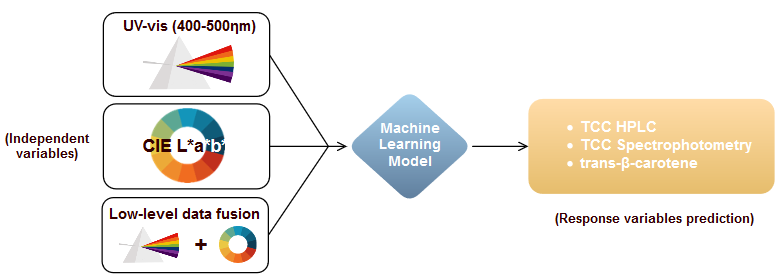
\includegraphics[width=1\linewidth]{Imagens/Case_study/ml_diagram}
	\caption{Machine learning approach used. Three different datasets were used as input to the models, namely the \gls{uv}, CIELAB and fusion datasets. The response variables used for prediction were the \gls{tcc} determined by spectrophotometry (Lambert-Beer law) and the \gls{tcc} and trans-$\beta$-carotene content determined by \gls{hplc}.}
	\label{ml_diagram}
\end{figure}

This being a regression problem, the chosen evaluation metrics to compare model performance were the \acrfull{rmse} and the coefficient of determination (R$^{2}$), since they explicitly show how much the model predictions deviate, on average, from the actual values in the dataset.


\subsubsection{UV-visible dataset}

Considering that most carotenoids exhibit absorption in the visible region of the spectrum, between 400 to 500 $\eta m$, a subset of the original \gls{uv} dataset was used, with samples belonging to this wavelength interval (101 features). Additionally, missing values contained within this dataset were replaced with the mean of the variables' values. 

Using the different response variables for prediction, the models that showed best performance were selected and the variable importance calculated. A set of pre-processing methods was applied to the datasets to see whether model performance could be improved, using the models that showed best performance with raw data. These pre-processing methods included smoothing interpolation, scaling, \acrfull{msc}, first derivative calculation and background, offset and baseline corrections. The data was also subject to filter-based feature selection (40\%, 60\% and 80\% data filtering) to determine if it could improve model performance.


\subsubsection{CIELAB dataset}
The analysis pipeline was similar for the CIELAB dataset, however, linear regression models with feature selection and the data pre-processing and filtering processes were excluded from the analysis pipeline, as it did not make sense to perform these, considering there are only 3 features in the dataset (L* a* and b* parameters), while pre-processing was meant for spectral data.

\subsubsection{Fusion dataset}
For the fusion dataset, which contained 104 variables (absorbance values + L* a* b* parameters), the analysis pipeline was similar to that of the CIELAB dataset, while data filtering was also performed similarly to the \gls{uv} dataset. For information regarding the data fusion process please see \autoref{data_fus}.

\subsubsection{Datasets Summary}

In \autoref{cassava_summary}, the summary of the different datasets used in this study is shown, giving an overall understanding of their composition. 

\begin{figure}[H]
	\centering
	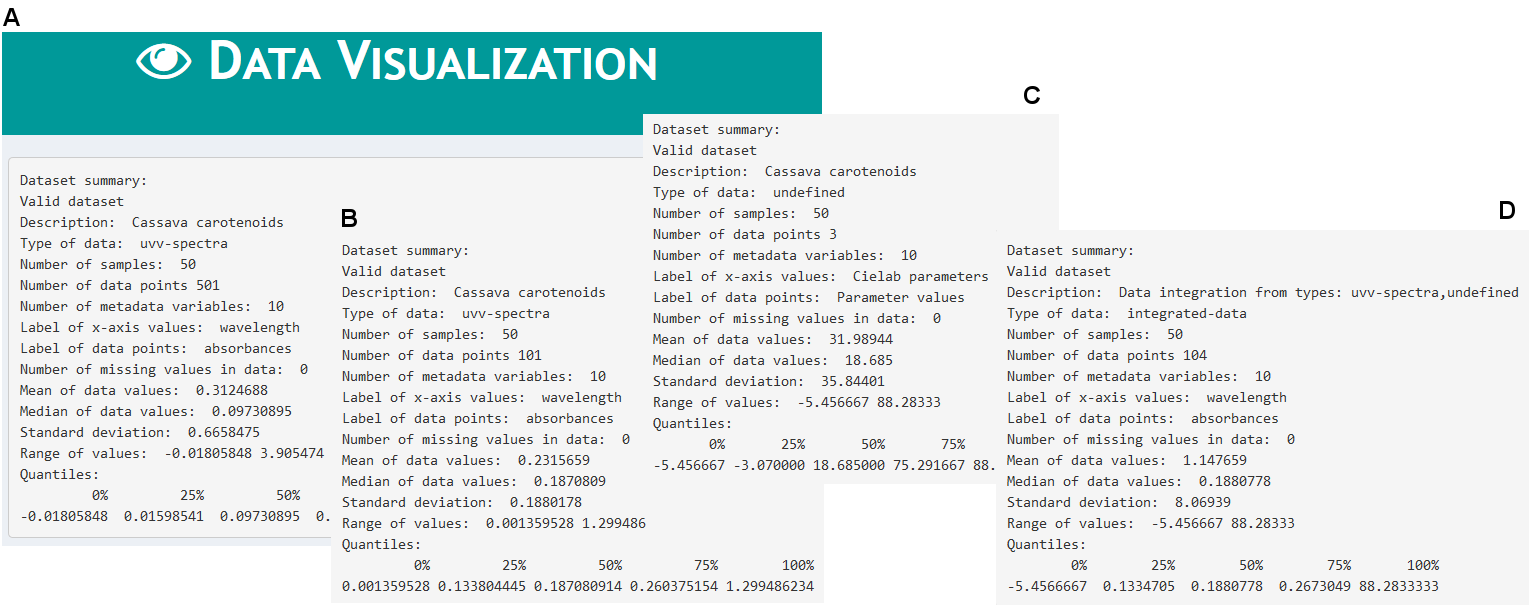
\includegraphics[width=1\linewidth]{Imagens/Case_study/summary_subset_full}
	\caption{Summary of the cassava full \gls{uv} dataset (\textbf{A}) and its subset (wavelengths between 400 and 500 $\eta m$) (\textbf{B}), the CIELAB dataset (\textbf{C}) and the fusion dataset (\textbf{D}), as seen in the web platform.}
	\label{cassava_summary}
\end{figure}

This includes the summary of the cassava full \gls{uv} dataset (\autoref{cassava_summary}A) and its subset with wavelengths between 400 and 500 $\eta m$ (\autoref{cassava_summary}B), the CIELAB dataset (\autoref{cassava_summary}C) and the fusion dataset (\autoref{cassava_summary}D). All datasets are valid, having no missing values, and therefore are ready for analysis.

All R scripts, raw data and additional analysis pipelines reports are available as supplementary material at \href{http://darwin.di.uminho.pt/pacbb2017/cassava-carotenoids/}{http://darwin.di.uminho.pt/pacbb2017/cassava-carotenoids/}, allowing full reproducibility of the experiments.


\section{Results and Discussion}  \label{results}

\subsection{Determination of carotenoid contents} \label{color_content_subsec}

The \gls{uv} spectrophotometric profiles measured between 200-700 $\eta m$ clearly allow us to discriminate samples according to their carotenoid content. This is more noticeable when comparing the typical \gls{uv} spectrophotometric profiles of cassava samples 5, 23 and 74 (\autoref{UV_spectra}). 


\begin{figure}[h]
	\centering
	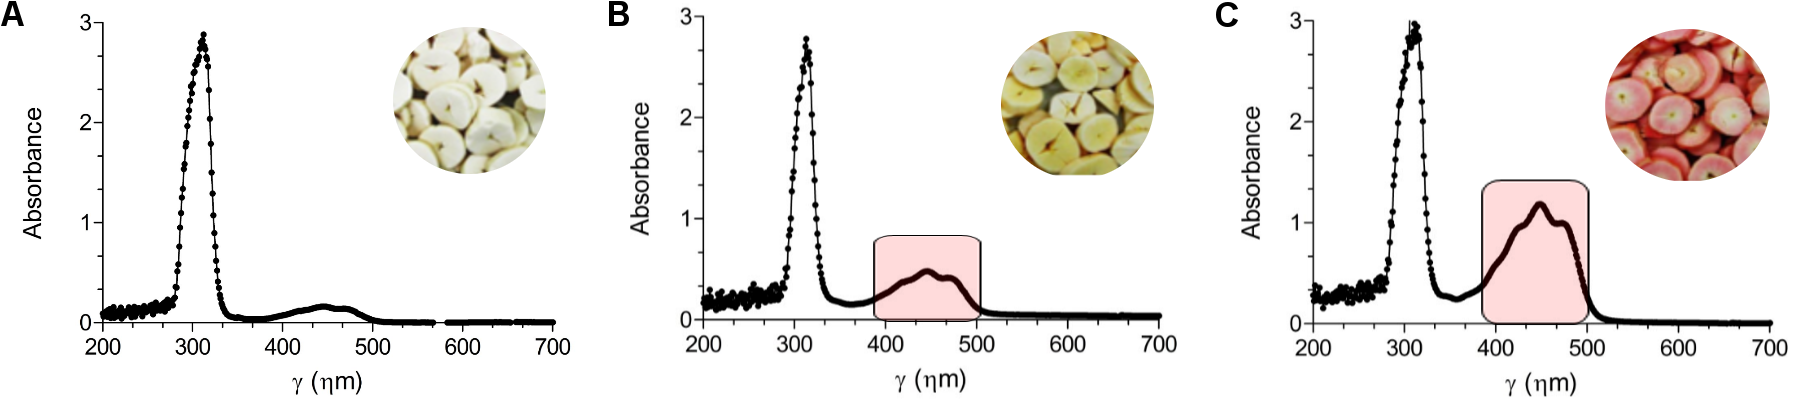
\includegraphics[width=1\linewidth]{Imagens/Case_study/UV_spectra_2}
	\caption{Typical \gls{uv} spectrophotometric profiles ($ \lambda $ = 200-700 $\eta m$, acetone: petroleum ether (v/v)) of root parenchymal tissues of three cassava samples: \textbf{A} - sample 5, \textbf{B} - sample 23 and \textbf{C} - sample 74. The 400-500$\eta m$ region of the spectrum is highlighted in cases \textbf{B} and \textbf{C}.}
	\label{UV_spectra}
\end{figure}

These three samples vary greatly in color, with sample 5 having a cream color, sample 23 a yellow one and the sample 74 a reddish color. In fact, the spectrophotometric profiles differ from each other only at 400-500$\eta m$ region of the spectrum, which is the region where carotenoids typically show absorbance peaks. 

The cream colored sample profile (\autoref{UV_spectra}A) shows an absence of absorbance peaks between the 400-500$\eta m$ region. On the other hand, the yellow colored sample profile (\autoref{UV_spectra}B) shows more noticeable peaks in this region, while the reddish colored sample (\autoref{UV_spectra}C) presents three peaks of great absorption in this region of the spectrum. It is, therefore, expected that the more colored the root the higher carotenoid content it possesses.

On the web platform, the same \gls{uv} spectrophotometric profiles for each sample could be observed in the \textit{Data Visualization} page, with many plot customization options (\autoref{cassava_spectra_plot}).


\begin{figure}[H]
	\centering
	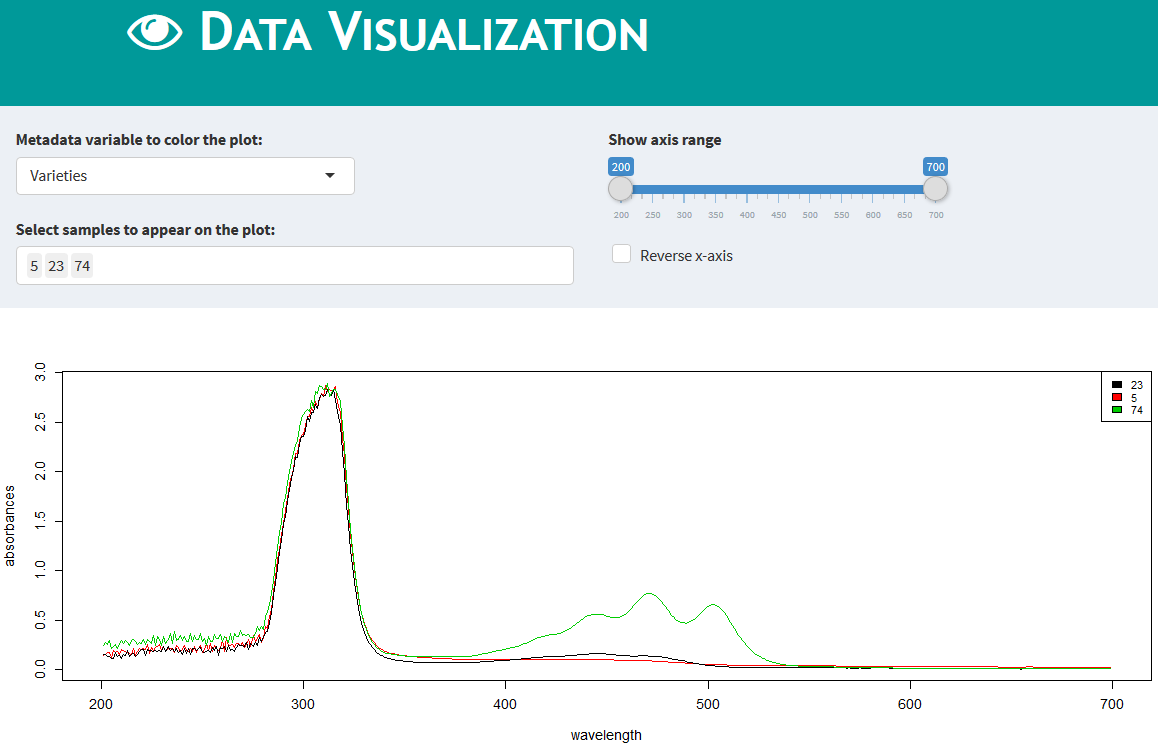
\includegraphics[width=0.8\linewidth]{Imagens/Case_study/spectra_plot}
	\caption{The \gls{uv} spectrophotometric profiles (200 to 700 $\eta m$) of cassava root sample 5 (red), sample 23 (black) and sample 74 (green), as seen on the web platform.}
	\label{cassava_spectra_plot}
\end{figure}


To confirm the possibility of the root color being correlated with its carotenoid contents, the \gls{tcc} was determined by \gls{uv} spectrophotometry, using the Lambert-Beer formula, and is shown in \autoref{carot_content_uv} for each of the fifty fresh root samples.

\begin{figure}[h]
	\centering
	\includegraphics[width=1\linewidth]{Imagens/Case_study/carot_content_uv}
	\caption{Concentration of total carotenoids ($\mu g.g^{-1}$ dry weight $\pm$ standard deviation) in samples of roots of fifty \textit{M. esculenta} genotypes, determined by \gls{uv} spectrophotometry (450 $\eta m$, $\varepsilon$ = 2592 $M^{-1} cm^{-1}$).}
	\label{carot_content_uv}
\end{figure}

A wide disparity in the carotenoid contents is observable, revealing the chemical variability among the analyzed genotypes. In the present study, the cream-colored roots showed the lowest concentrations of total carotenoids, with values around 0.57 $\mu g.g^{-1}$, while higher concentration values were measured in yellow and reddish pigmented roots i.e, 54.93 $\mu g.g^{-1}$. The most abundant carotenoids, trans-$\beta$-carotene and cis-$\beta$-carotene, had concentration values that ranged from 1.82 to 42.82 $\mu g.g^{-1}$ and from 1.19 to 28.86 $\mu g.g^{-1}$, respectively. The results from the \gls{hplc} carotenoid quantification are available in the metadata file.

These findings altogether are consistent with data reported in the literature that observe a positive correlation between the color of the root pulp and the total carotenoid content \citep{champagne2010carotenoid, chavez2005variation, iglesias1997genetic}.


\subsection{CIELAB color space interpretation} \label{cielab_subsec}

To better understand the correlation between samples and the different types of carotenoids with the CIELAB color space, the observed values of L*, a* and b* for each root sample were projected into the CIELAB plane \citep{kljak2014reflectance}. 
The visual interpretation of \autoref{cielab_plot}, showing samples location according to the color of roots in the CIELAB color space, is already sufficient to verify which samples possess higher carotenoid amounts.


\begin{figure}[h]
	\centering
	\includegraphics[width=0.7\linewidth]{Imagens/Case_study/cielab_plot2}
	\caption{Location of the cassava samples in the CIELAB color space according to their root pulp colors. The a* value characterizes the coloration in the regions of red (+a*) to green (-a*). The value b* indicates coloring in the range of yellow (+b*) to blue (-b*). Sample identifiers in ellipse II were omitted for easier interpretation of the plot.}
	\label{cielab_plot}
\end{figure}


Samples 105, 119 and 125 (\autoref{cielab_plot}, ellipse I) show high b* values, which stands for the coloration in the yellow range, and these are in fact the samples with the highest carotenoid contents, as it can be observed in \autoref{carot_content_uv}. Interestingly, sample 74 (\autoref{cielab_plot}, ellipse IV) is deviated into the positive axis of a*, which corresponds to the red coloration. In fact, this sample is a reddish root, mostly due to its lycopene content, which confers reddish coloration to the biomass \citep{melendez2007relationship}. It is one of the samples with the highest carotenoid concentration (\autoref{carot_content_uv}).

Samples 123, 27, 05, and AO47 (\autoref{cielab_plot}, ellipse III) were grouped in values of b* closer to zero, these being the samples with the lowest carotenoid content (\autoref{carot_content_uv}). The remaining samples had medium and more similar carotenoid content, being grouped together in a* negative and b* positive values (\autoref{cielab_plot}, ellipse II).


\subsection{Principal Components Analysis} 

The similarity patterns of carotenoid composition found in the previous section were also present among the evaluated genotypes through a \gls{pca} (\autoref{pca_plot}). Information regarding this method is available in \autoref{unsupervised}. 

\begin{figure}[h]
	\centering
	\includegraphics[width=0.7\linewidth]{Imagens/Case_study/pca_plot_3}
	\caption{Scores plot with the distribution of the fifty samples on the first and second \gls{pca} components resulting from the \gls{uv} spectrophotometric data (400-500 $\eta m$), as seen on the web platform. To facilitate the interpretation of the plot, only the sample identifiers for the most relevant samples are shown.}
	\label{pca_plot}
\end{figure}


PC1 and PC2 explain about 99.5\% of the total variance of the sample population data under this study. The performed \gls{pca} resulted in genotype grouping according to the root pulp coloration, as well as carotenoid quantification, with samples 74, 105, 119, and 125 being the most discrepant within this sample universe (\autoref{pca_plot}). 

These being the samples with the highest carotenoid content show that the results here obtained are in accordance with the findings in \autoref{color_content_subsec} that positively correlate the carotenoid content with the color of the cassava roots.


\section{Univariate Analysis} \label{univ_analysis}

To detect significant statistical differences (p-value below 0.05) derived from the effects of cassava's root colors on the spectral profiles, a one-way \gls{anova} with Tukey's \gls{hsd} analysis was performed for all wavelengths (200 to 700 $\eta m$). More information about these methods is available in \autoref{univariate}.

For this, the discrete \textit{colors} metadata variable was used, containing the visually determined color of the roots (5 levels:  \textit{Cream}, \textit{DeepYellow}, \textit{Reddish}, \textit{White} and \textit{Yellow}). \autoref{cassava_anova}A shows the top ten results ordered by decreasing p-values. In \autoref{cassava_anova}B,  the -log$_{10}$ of p-values plot is represented, showing an horizontal line that corresponds to a p-value threshold of 0.05. 

\begin{figure}[h]
	\centering
	\includegraphics[width=1\linewidth]{Imagens/Case_study/anova_table_plot}
	\caption{\gls{anova} results using the discrete \textit{colors} metadata variable (\textbf{A}) and respective plot of the -log$_{10}$ of p-values with a p-value threshold value of 0.05 (\textbf{B}), as seen on the web platform.}
	\label{cassava_anova}
\end{figure}

From \autoref{cassava_anova} it appears that wavelengths around 500$\eta m$ have a significant effect on the discrimination of cassava samples according to their color. This finding becomes more evident when looking at the -log$_{10}$ of p-values plot.


\section{Machine Learning}

\subsection{Carotenoid content prediction using \gls{uv} data} \label{ml_uv_subsec}

In \autoref{UV_table}, the performance values obtained with the various machine learning models using \gls{uv} data (400-500 $\eta m$) as input and the \gls{tcc} determined by spectrophotometry (Lambert-Beer formula), the \gls{tcc} determined by \gls{hplc} and the total content of trans-$\beta$-carotene (the most abundant carotene in cassava roots) as response prediction variables are shown.


\begin{table}[h]
	\centering
	\caption{Performance values (\gls{rmse} and $R^{2}$) obtained for the different machine learning models trained with \gls{uv} spectrophotometry data (400-500 $\eta m$). The \acrfull{tcc} determined by spectrophotometry (Lambert-Beer formula), the \gls{tcc} determined by \gls{hplc} and the total content of trans-$\beta$-carotene (the most abundant carotene in cassava roots) were used as response prediction variables. The parenthesis indicate the package specific method chosen for the simulation, with exception to the linear regression models.}	
	\includegraphics[width=1\linewidth]{Imagens/Case_study/UV_table}
	\label{UV_table}
\end{table}


The highest $R^{2}$ performance values (above 90\%) and lowest \gls{rmse} values were obtained when using the \gls{tcc} determined using spectrophotometric data as response variable. This was expected considering that both input and response data used employ the same physical phenomenon of detection of compounds (absorbance). The models that best performed in this case were \gls{pls} using both \textit{simpls} and \textit{widekernelpls} methods, \gls{svm}s and random forests with \gls{rmse} performance values of 3.492, 3.732, 3.709 and 3.768, respectively.

Using the \gls{tcc} determined by \gls{hplc} as the response variable, a small decrease in performance values is observed, with \gls{pls} (\textit{widekernelpls} and \textit{pls} methods) and elastic network showing best performance with \gls{rmse} values of 5.779, 5.643 and 5.934, respectively, and $R^{2}$ values around 60\%.

The worst results were obtained when using trans-$\beta$-carotene as response variable, with best performance models being \gls{pls} (\textit{widekernelpls} and \textit{pls} methods) and \gls{svm}s, with \gls{rmse} values of 4.324, 4.265 and 4.230, respectively, and $R^{2}$ values around 46\%.

When observed, the values of \acrfull{vip} for this analysis (supplementary material), which identify the most relevant variables for the validation of the method, it can be detected that the wavelengths 449, 448 and 450 nm (precisely the wavelength that is used for the quantification of $\beta$-carotene through the Lambert-Beer formula) were used in 100\%, 99.93\% and 99.76\% of cross-validation training performance. This result is important in the sense that it attests to the robustness of the models in predicting the contents of these compounds in cassava samples.

By pre-processing the data, as well as applying feature selection, an overall increase in model performance for most models used was observed (supplementary material). In \autoref{UV_preproc_table}, one such case is shown, where using pre-processed \gls{uv} data as input to Random Forest model (best performing model with raw data) increased even further model performance. By applying smoothing interpolation, background and offset corrections, or background correction alone, \gls{rmse} values decreased from 6.194 to 5.773, 5.936 and 6.175, respectively. $R^{2}$ values also increased from 55\% to around 60\% in each case.


\begin{table}[h]
	\centering
	\caption{Performance values (\gls{rmse} and $R^{2}$) obtained for a random forest model trained with \gls{uv} spectrophotometry data (400-500 $\eta m$), applying several pre-processing methods to the data. The \gls{tcc} determined by \gls{hplc} was used as response prediction variable.}	
	\includegraphics[width=0.8\linewidth]{Imagens/Case_study/UV_preproc_table}
	\label{UV_preproc_table}	
\end{table}


\subsection{Carotenoid content prediction using CIELAB data} \label{ml_cielab_subsec}

The performance values obtained by using CIELAB data as input to the various machine learning models are shown in \autoref{CIELAB_table}. The \gls{tcc} determined by spectrophotometry (Lambert-Beer formula), the \gls{tcc} determined by \gls{hplc} and the total content of trans-$\beta$-carotene (the most abundant carotene in cassava roots) were used as response prediction variables.


\begin{table}[h]
	\centering
	\caption{Performance values (\gls{rmse} and $R^{2}$) obtained for the different machine learning models trained with CIELAB data. The \gls{tcc} determined by spectrophotometry (Lambert-Beer formula), the \gls{tcc} determined by \gls{hplc} and the total content of trans-$\beta$-carotene (the most abundant carotene in cassava roots) were used as response prediction variables. The parenthesis indicate the package specific method chosen for the simulation.}	
	\includegraphics[width=1\linewidth]{Imagens/Case_study/CIELAB_table}
	\label{CIELAB_table}	
\end{table}


Similarly to the results obtained in \autoref{ml_uv_subsec}, highest $R^{2}$ performance values and lowest \gls{rmse} values were obtained when using the \gls{tcc} determined using spectrophotometric data as a response prediction variable. There is, however, a noticeable overall decrease in model performance when using all three prediction variables. This is easily explained by the number of features present in the data, considering that in this case only three features are present (L*, a* and b*), while in the previous case there were far more features, about 101 (data measured from 400 to 500$\eta m$).

Using the \gls{tcc} determined by spectrophotometry as response variable, the models that showed best performance were linear and ridge regressions and elastic network with \gls{rmse} values of 6.295, 6.417 and 6.456, respectively, with $R^{2}$ values around 60\%. 

For the second variable, \gls{tcc} determined by \gls{hplc}, the best models were elastic network, ridge regression and \gls{svm}s with \gls{rmse} values of 6.534, 6.584 and 6.534, respectively, and $R^{2}$ values around 40\%. 

Lower \gls{rmse} values were observed when using trans-$\beta$-carotene as response variable, with best performance models being \gls{pls} (\textit{widekernelpls} and \textit{pls} methods) and conditional inference random forests, with \gls{rmse} values of 4.551, 4.667 and 4.667, respectively. However, models showed a decrease in the fitting of the data with an $R^{2}$ around 25\%.

Looking at the \gls{vip} (supplementary material), the variables that played the most important role in the prediction of carotenoid content in the cassava samples are evident. The b* parameter was relevant about 100\% of the cases, which was somewhat expected, considering that the samples are widely distributed across the \textit{y} axis in \autoref{cielab_plot}, which corresponds to the b* parameter. Looking at the same plot we can see that the a* interval in which samples are distributed is not as wide, however, this parameter was relevant in about 56\% of the predictions. With a VIP of 0\% the L* parameter was the least relevant of the three.

The only pre-processing method applied to CIELAB data was scaling, as the other methods would not make much sense considering they are aimed at spectral data. Applying the scaling to the data showed an increase in model performance, however limited (supplementary material).



\subsection{Carotenoid content prediction using fusion data} \label{ml_fusion_subsec}

The performance values obtained by using a \gls{llf} between \gls{uv} (400-500 $\eta m$) and CIELAB data as input to the various machine learning models are shown in \autoref{UV_cielab_table}. Similarly to the previous cases, the response prediction variables used were the \gls{tcc} determined by spectrophotometry (Lambert-Beer formula), the \gls{tcc} determined by \gls{hplc} and the total content of trans-$\beta$-carotene.


\begin{table}[h]
	\centering
	\caption{Performance values (\gls{rmse} and $R^{2}$) obtained for the different machine learning models trained with a fusion between \gls{uv} spectrophotometry and CIELAB data. The \gls{tcc} determined by spectrophotometry (Lambert-Beer formula), the \gls{tcc} determined by \gls{hplc} and the total content of trans-$\beta$-carotene (the most abundant carotene in cassava roots) were used as response prediction variables. The parenthesis indicate the package specific method chosen for the simulation, with exception to the linear regression models.}	
	\includegraphics[width=1\linewidth]{Imagens/Case_study/UV_cielab_table}
	\label{UV_cielab_table}	
\end{table}


The results obtained for fusion data are similar to those in \autoref{ml_uv_subsec} and \autoref{ml_cielab_subsec} in the sense that highest $R^{2}$ performance values and lowest \gls{rmse} values were obtained when using the \gls{tcc} determined using spectrophotometric data as response prediction variable. Overall there is an increase in model performance when comparing to the results obtained for \gls{uv} data alone.

The best model performance when using the \gls{tcc} determined by spectrophotometry as response variable was achieved by ridge regression (with feature selection) and \gls{pls} (\textit{pls} and \textit{simpls} methods) models with \gls{rmse} values of 3.570, 3.682 and 3.706, respectively, and $R^{2}$ values around 90\%.

For the variable \gls{tcc} determined by \gls{hplc}, the models that best performed were ridge regression (with feature selection) and \gls{pls} (\textit{kernelpls} and \textit{widekernelpls}) models, having \gls{rmse} values of 5.981, 6.010 and 6.031, respectively, with $R^{2}$ values around 50\%.

Similarly to the previous cases, lower \gls{rmse} values were observed when using trans-$\beta$-carotene as prediction variable, with best performance models being SVMs (\textit{e1071} and \textit{kernlab} methods) and elastic network with \gls{rmse} values of 4.353, 4.436 and 4.450, respectively, and $R^{2}$ values around 30\%.

The \gls{vip} computed for this case (supplementary material) showed that the variables which presented the most important role in the prediction of carotenoid content in the cassava samples were those of wavelength around 170$\eta m$ (VIPs $>$ 99\%). Here, the CIELAB b* parameter was relevant in about 65\% of predictions, while the a* and L* parameters had a VIP close to zero.

The only preprocessing method applied to the fusion data was scaling, as the methods employed in \autoref{ml_uv_subsec} are aimed at spectral data. Data filtering was also applied to the data. Both methods contributed to an overall increase in model performance when compared to the performance obtained using raw \gls{uv} data (supplementary material).


\section{Conclusions} \label{conclusions}

The present study has shown how CIELAB color measurement can be used as a fast and non-destructive method to calibrate for the total carotenoid content of cassava genotypes roots with acceptable prediction error. The  \gls{llf} of \gls{uv} spectrophotometry and CIELAB data has demonstrated how data fusion can lead to a better model performance for prediction when comparing to the use of a single data source, having similar results been found in the literature \citep{botwey2014multi}.

Furthermore, the \gls{uv} spectrophotometric profiles measured between 400-500$\eta m$ and the consequent carotenoid content determination allowed the observation of a positive correlation between the color of the root pulp and the \gls{tcc}, which is in accordance with data reported in the literature \citep{champagne2010carotenoid, chavez2005variation, iglesias1997genetic}. This finding was more explicit when observing the projection of the fifty cassava root samples in the CIELAB color space plane, having several clusters been formed, where the highest values of b* (which stands for the yellow coloration) and a* (which stands for the red coloration) were associated to the samples with highest carotenoid contents.

Additionally, the information obtained by coupling the analysis of pro-vitamin A biochemical markers to bioinformatics tools helps supporting the rational design of biochemically-assisted breeding programs of \textit{M. esculenta}, that aim to obtain cultivars with high levels of pro-vitamin A carotenoids and superior nutritional traits.















	
	
	% BIBLIOGRAPHY ----------------------
	
	\bibliographystyle{apalike}
	\bibliography{dissertation}


	

\end{document}
